% !TEX root=./dummy-03.tex

\chapter{双杂化泛函的电性质梯度理论与程序实现}
\label{sec.3.title}

\section{引言}

表征技术是实验科学问题的重要分支之一。对于化学而言,经典的 IR、UV-Vis、Raman、NMR 等表征手段被合称为“四大光谱”\footnote{“四大光谱”的说法并不是正式的。也有将其中一类谱替换为 MS 或 XRD 等。正文中说道计算化学对谱学问题有所帮助;但并不是所有谱学问题都与电子结构有紧密的关系、基于第一性的计算化学也未必能解决或解释所有谱学问题。例如 MS 与分子构型关联度更大、XRD 与晶格本身更有关、通过计算化学难以给出色谱的保留时间等。},在以有机化学为代表的分支学科中是必要的佐证手段。近年来,STM、\emph{in situ} IR、SERS、SEM 等众多新兴表征手段兴起。由于其中的许多表征问题可以归结为电子结构或分子振动效应,因此可以或有希望通过第一性的计算化学方法计算得到,从而实验与理论或计算可以相互印证,推动化学学科的发展。

在第 \alertref{sec.1.title}、\alertref{sec.2.title} 章中已经表明密度泛函方法,特别是双杂化密度泛函近似,在基态能量计算上有较好的表现。我们预期在谱学计算上,双杂化密度泛函方法也能有良好的表现。为此,我们需要发展双杂化泛函的谱学计算方法。由于较多光谱问题 (包括 IR、Raman、NMR 等) 可以归结为偶极电场或磁场 $\symbfscr{E}$ 下平衡态分子的基态能量 $E(\symbfscr{E})$ 扰动问题,其中 $\symbfscr{E}$ 为微扰外场;那么光谱的强度经常取决于导数量
\begin{equation}
    \lim_{|\symbfscr{E}| \rightarrow 0} \frac{\mathrm{d}^n E(\symbfscr{E})}{\mathrm{d} \symbfscr{E}^n}
\end{equation}
或其导出量、或多种外场下的混合导数量。光谱问题也经常与分子振动有关;若上式的外场 $\symbfscr{E}$ 替换为原子坐标移动向量,那么分子振动将化归为 $n = 2$ 即二阶导数问题。对于这类光谱计算问题,为通过计算化学手段进行模拟,我们需要对能量在外场下的梯度理论作研究与程序化。我们也称可以化归为梯度计算的光谱或振动问题为\textbf{梯度性质}问题。

双杂化泛函的梯度性质已经有先驱性的程序实现与测评\cite{Neese-Grimme.JCP.2007, Biczysko-Barone.JCTC.2010, Su-Xu.JCC.2013, Stoychev-Neese.JCTC.2018, Gu-Xu.JCTC.2021, Yan-Xu.JCTC.2022}。这些工作表明,双杂化泛函,特别是 xDH 型泛函,在分子振动、NMR 光谱预测等问题上有优异的表现。但目前的程序在计算双杂化解析梯度问题上,效率还一定提升空间。同时,考虑到双杂化泛函除了 MP2 型相关能外还有其它的杂化可能性;在理论推导与程序化过程中,也应尽量留出空间以容纳其它杂化形式。

基于前人的工作\cite{Gerratt-Mills.JCP.1968, Gerratt-Mills.JCP.1968a, Pople-Binkley.IJQC.1979, Dykstra-Jasien.CPL.1984, Handy-Schaefer.JCP.1984, Handy-Simandiras.CPL.1985, Pulay-Saeboe.TCA.1986, Trucks-Bartlett.CPL.1988, Frisch-Pople.CP.1990, Frisch-Pople.CPL.1990, Frisch-Pople.CPL.1990a, Gauss-Bartlett.JCP.1992, Stanton-Bartlett.CPL.1992, Johnson-Frisch.CPL.1993, Head-Gordon-Head-Gordon.CPL.1994, Yamaguchi-Schaefer.Oxford.1994, Weigend-Haeser.TCA.1997, Aikens-Gordon.TCA.2003, Cammi-Frisch.TCA.2004, Distasio-Head-Gordon.JCC.2007, Neese-Grimme.JCP.2007, Biczysko-Barone.JCTC.2010, Su-Xu.JCC.2013, Ji-Jung.JCTC.2013, Bykov-Neese.MP.2015, Stoychev-Neese.JCTC.2018, Gu-Xu.JCTC.2021, Yan-Xu.JCTC.2022},将以电性质外场微扰为前提下,进行双杂化二阶梯度梯度的理论推演、与基于原子轨道基的程序化。本章节的内容自成完整的篇章。本章的理论推演部分是其他科研工作者已有成果的总结与重新复述,\textbf{并非独创性工作};程序编写在 \textsc{PySCF} 程序的基础上独立完成。为清晰地表述程序实现思路与原则,在复述电性质二阶梯度理论时,本文着重于
\begin{itemize}[nosep]
    \item 一般不使用波函数,避免大量使用矩阵或张量记号、尽量使用展开了指标的矩阵或张量元素记号 (同时参见文献 \citenum{Aikens-Gordon.TCA.2003}),并一定程度地规范指标记号 (参见 \ref{sec.3.notations} 节);
    \item 对于 DFT 格点计算,也尽量使用张量记号展开密度在空间坐标上的数值;
    \item 文段自成篇章,尽可能展示诸多张量的定义,减少未定义记号的出现;
    \item 强调现有流行的密度泛函、其能量泛函 $E^\textmt{DH}$ 及其导出量的可加和性,即它是诸多能量贡献项的线性加和;在初步的理论推演中,弱化每个能量项的表达细节以求适用性更宽泛的表达式;在程序实现中,这些能量贡献具体展开为可扩展的实例列表。
\end{itemize}
\ref{sec.3.basic-equation-def} 与 \ref{sec.3.dipole-polar} 节对计算化学与电性质的基本概念的记号作定义。\ref{sec.3.theory} 节对双杂化泛函电性质梯度涉及到的记号作定义;这节内容不引入具体的 MP2 相关能,因此预期可以推广到包含长短程的 MP2 型相关能、或者其他相关能形式的双杂化泛函,使得程序可以有灵活的框架。\ref{sec.3.program} 节解释了本工作中,闭壳层 MP2 相关能构成的双杂化泛函的程序实现细节与思路。\ref{sec.3.efficiency} 节通过简单的例子,展示本工作程序的实现效率。本工作的梯度实现是基于弱的正则 SCF 条件 (\ref{eq.3.weak-canonical-SCF});作为附录的 \ref{sec.3.non-canonical-mp2-gradient} 节展示当前记号体系下,非正则 MP2 相关能及其梯度的推演过程。

% \ref{sec.3.background} 节将介绍物理问题背景与程序化背景,以确定大体的技术线路。\ref{sec.3.theory} 节将介绍一般双杂化泛函电性质解析梯度理论。MP2 型泛函作为双杂化泛函的其中一个重要的分支,其在 RI 近似下解析静态极化率的 Python 代码在 CPU 上的实现细节将在 \ref{sec.3.program} 阐述,并作简单的效率测评。

\section{记号}
\label{sec.3.notations}

\subsection{约定俗成}

\subsubsection{字母记号}

\begin{table}[!ht]
\centering
\caption[字母记号与指标约定俗成]{字母记号与指标约定俗成。}
\label{tab.A.notation-suxscript}
\widetabular{
    \begin{tabular}{llcll}
    \toprule
    字母记号 & 记号意义 & 标记 & 字集 & 字体 \\
    \midrule
    $\phi$ & 原子轨道 & 标量函数 & 特定 & 斜体 \\
    $\mu, \nu, \kappa, \lambda, \eta$ & 原子轨道 (基轨道) & 下标 & 希腊 & 斜体 \\
    $i, j, k, l$ & 占据分子轨道 & 下标、标量函数 & 小写 & 斜体 \\
    $a, b, c$ & 非占分子轨道 & 下标 & 小写 & 斜体 \\
    $p, q, r, s, m$ & 任意分子轨道 & 下标 & 小写 & 斜体 \\
    $P, Q, R, S$ & RI 辅助基轨道 & 下标 & 大写 & 斜体 \\
    $A, B, M$ & 原子核 & 下标 & 大写 & 斜体 \\
    $\bm{A}, \bm{B}$ & 原子核坐标 & 三维向量 & 大写 & 粗斜体 \\
    $\bm{r}$ & 电子坐标 & 三维向量 & 特定 & 粗斜体 \\
    $\bm{x}$ & 电子自旋坐标 & 四维向量 & 特定 & 粗斜体 \\
    $w, t$ & 坐标分量 (用于指代 $x, y, z$) & 上下标 & 小写 & 斜体 \\
    $\sigma, \varsigma$ & 自旋 (指代 $\alpha, \beta$) & 上标 & 希腊 & 斜体 \\
    $\rho$ & 电子云密度 & 标量函数 & 特定 & 斜体 \\
    $\gamma$ & 电子云密度的梯度导出量 & 标量函数 & 特定 & 斜体 \\
    $\chi$ & 电子云密度导出量 & 下标、标量函数 & 希腊 & 斜体 \\
    $\mathrm{n}$ & 非变分 (相对于自洽场泛函) & 上标 & 特定 & 正体 \\
    $\mathrm{S}$ & skeleton 导数 & 上标 & 特定 & 正体 \\
    $\mathrm{U}$ & 轨道旋转导数 & 上标 & 特定 & 正体 \\
    $\textmt{x}$ & 交换效应 & 下标 & 特定 & 非衬线 \\
    $\textmt{c}$ & 相关效应 & 下标 & 特定 & 非衬线 \\
    $g$ & 空间离散格点 & 下标 & 小写 & 斜体 \\
    $\symbb{A}, \symbb{B}$ & 外场微扰量、被求导量 & 下标、向量 & 大写 & 双线体 \\
    $\symbfscr{E}$ & 偶极电场 & 上下标、三维向量 & 特定 & 粗花体 \\
    \bottomrule
    \end{tabular}
}{}
\end{table}

表 \ref{tab.A.notation-suxscript} 给出本工作的记号与指标约定俗成。在该表基础上,对于开壳层问题,为简化记号,不同自旋下的轨道通过上标横线区分 ($p$ 表示 $\alpha$ 自旋、$\bar p$ 表示 $\beta$ 自旋),矩阵或张量则将上标具体的自旋。没有上标横线的情形可能是闭壳层轨道或自旋轨道,这两类情况本工作不用记号加以区分;除非特别指明,若并非开壳层问题,则轨道记号指代闭壳层情形。

部分指标会上标波浪线 (如 $t_{\tilde{i} j}^{ab}$)。这是在程序实现中,对该指标作分批处理。

\subsubsection{特殊符号}

\begin{itemize}[nosep]
    \item $\coloneq$ (冒号等号符号):表达式定义;
    \item $\simeq$ (近似等于符号):涉及 RI 近似的情形;
    \item $\doteq$ (点等于符号):涉及 DFT 格点积分的情形;
    \item $\sim$ (相似符号):计算复杂度的正比渐进;
    \item $\leftarrow$ (左箭头符号):对左侧表达式产生线性加和的贡献项;
    \item $\not \equiv$ (非恒等符号):表达式可能是、但不总是等于特定常数。
\end{itemize}

\subsubsection{数量记号}

\begin{itemize}[nosep]
    \item $N$:一种大概的、正比于体系大小的数量;
    \item $n_\mathrm{basis}$:基函数数量;
    \item $n_\mathrm{orb}$:分子轨道数量;
    \item $n_\mathrm{occ}$:闭壳层下占据轨道数量;
    \item $n_\mathrm{vir}$:闭壳层下非占轨道数量;
    \item $n_\mathrm{aux}$:辅助基函数数量;
    \item $n_\mathrm{prop}$:外场向量大小;
    \item $n_\mathrm{slice}(i)$:对 $i$ 指标的分割数。
\end{itemize}

\subsubsection{其他记号规则}

\begin{itemize}[nosep]
    \item 粗斜体或粗花体表示一维向量;
    \item 粗体表示二维矩阵或高维向量;
    \item 非衬线体表示近似方法或分量的物理意义;
    \item 在不引起歧义的情况下,将使用矩阵或张量元素指代矩阵或张量本身,例如用 $D_{\mu \nu}$ 表示完整的自洽场密度矩阵 $\mathbf{D}$;
\end{itemize}

本工作的全部理论推导与程序实现使用实数;正文中不涉及对偶空间的概念。为简化公式表达,将不使用复共轭记号;二维矩阵上标 $\dagger$ 仅表示转置。通常使用 $\phi_\mu (\bm{r})$ 表示原子轨道 $\mu$ 在空间坐标 $\bm{r}$ 下的函数表达式。对于 DFT 格点积分,若记坐标在指标 $g$ 下的离散格点为 $\bm{r}_g$,那么也经常用 $\phi_{g \mu}$ 作为二阶张量表示空间格点下的原子轨道函数值 $\phi_\mu (\bm{r}_g)$。

涉及近似计算复杂度的部分,本工作仅作简单分析,并统一使用大 O 记号。

\subsection{变种的 Einstein 求和记号}
\label{sec.3.einstein}

出于简化公式表达,在本章节中,将对张量缩并大量使用变种的 Einstein 求和记号\cite{Einstein-Einstein.AP.1916}。

在该求和记号下,对于本工作中公式最左侧的等号,等式的左边没有出现的指标,将在等式右边对这些指标作乘积并求和;等式左边出现的指标,则在等式右边作数乘。对照表 \ref{tab.A.notation-suxscript},本工作所涉及的被求和指标,其字集必是大写、小写或希腊,其字体必是斜体。本文档的公式所使用的变种 Einstein 求和记号,会比较接近于具体程序实现时的情形,并允许打破一些物理记号的限制。

作为一些例子,下述列表的推出号 ($\Rightarrow$) 左边是正常的求和记号,右边是变种的 Einstein 求和记号:
\begin{itemize}[nosep]
\item \textbf{普通的求和。}以 Fock 矩阵自原子轨道基到分子轨道基的变换为例,
\begin{equation}
    F_{pq} = \sum_{\mu \nu} C_{\mu p} F_{\mu \nu} C_{\nu q}
    \Rightarrow
    F_{pq} = C_{\mu p} F_{\mu \nu} C_{\nu q}
\end{equation}
等式左边有指标 $p, q$,但没有指标 $\mu, \nu$;因此等式右边就对 $\mu, \nu$ 作求和。需要注意到,通常的 Einstein 求和需要定义在对偶空间下;指标 $\mu, \nu$ 并非表示相同的基,而是分别表示对偶两空间的基 (对于 $p, q$ 同理);相互对偶的空间指标分别写为上下标。因此,上式在通常的 Einstein 求和下应写为
\begin{equation*}
    F^p_q = C^p_\mu F^\mu_\nu C^\nu_q
\end{equation*}
\item \textbf{特殊形式下标的求和。}以 ERI 积分自原子轨道到分子轨道的变换为例,
\begin{equation}
    (ia|jb) = \sum_{\mu \nu \kappa \lambda} C_{\mu i} C_{\nu a} (\mu \nu | \kappa \lambda) C_{\kappa j} C_{\lambda b}
    \Rightarrow
    (ia|jb) = C_{\mu i} C_{\nu a} (\mu \nu | \kappa \lambda) C_{\kappa j} C_{\lambda b}
\end{equation}
在本工作中,$(ia|jb)$ 的指标 $i, a, j, b$ 尽管以普通斜体字母出现,但它们均将被视为下标。若将 $(ia|jb)$ 记为 $g_{ij}^{ab}$、$(\mu \nu | \kappa \lambda)$ 记为 $g_{\mu \kappa}^{\nu \lambda}$,那么上式在通常的 Einstein 求和下应写为
\begin{equation*}
    g_{ij}^{ab} = C_i^\mu C^a_\nu g_{\mu \kappa}^{\nu \lambda} C_j^\kappa C^b_\lambda
\end{equation*}
\item \textbf{带有数乘的求和。}以电子云密度在原子轨道基下的矩阵到空间格点计算过程为例,
\begin{equation}
    \rho_g = \sum_{\mu \nu} D_{\mu \nu} \phi_{g \mu} \phi_{g \nu}
    \Rightarrow
    \rho_g = D_{\mu \nu} \phi_{g \mu} \phi_{g \nu}
\end{equation}
该式等式左右都包含代表空间位置的指标 $g$;该指标在等式右边被数乘,而没有最终被求和。由于 $g$ 指标并非在对偶空间中,因此若不将 $g$ 看做指标,那么在通常的 Einstein 求和下应写为
\begin{equation*}
    \rho_g = (\phi_g)_\mu D^\mu_\nu (\phi_g)^\nu
\end{equation*}
\item \textbf{带有加减过程的求和。}以双杂化密度的 Lagrangian 求取过程为例,
\begin{align}
    \label{eq.3.einsum-4}
    L_{ai}^\textmt{DH} &= - (\varepsilon_a - \varepsilon_i) Z_{ai}^\textmt{DH} - \sum_{bj} A_{ai, bj} Z_{bj}^\textmt{DH} \notag\\
    \Rightarrow
    L_{ai}^\textmt{DH} &= - (\varepsilon_a - \varepsilon_i) Z_{ai}^\textmt{DH} - A_{ai, bj} Z_{bj}^\textmt{DH}
\end{align}
对于该式,$\textmt{DH}$ 并非是斜体指标;被求和的指标 $b, j$ 仅针对其所在的项 $A_{ai, bj} Z_{bj}^\textmt{DH}$ 进行,而不对其他项 $\varepsilon_a Z_{ai}^\textmt{DH}$ 与 $\varepsilon_i Z_{ai}^\textmt{DH}$ 进行。该式在通常的 Einstein 求和下应写为
\begin{equation*}
    (L^\textmt{DH})_a^i = - F_a^b (Z^\textmt{DH})_b^i + F_j^i (Z^\textmt{DH})_a^j - A_{aj}^{ib} (Z^\textmt{DH})_b^j
\end{equation*}
上式的 $F_p^q$ 是 Fock 分子轨道基下的矩阵,在正则 Hartree-Fock 轨道下等于 $\delta_{pq} \varepsilon_p$。事实上,上式通常的 Einstein 求和记号对非正则 Hartree-Fock 也成立,但式 (\ref{eq.3.einsum-4}) 的变种 Einstein 求和记号只对正则 Hartree-Fock 有意义。强制使用通常的 Einstein 求和记号更符合求取 Lagrangian 本来的意义;但使用变种的 Einstein 求和跟接近程序实现的思路。
\item \textbf{带有直和的求和。}以自旋轨道下 MP2 相关能计算为例,
\begin{equation}
    E_\textmt{c}^\textmt{(2)} = - \frac{1}{4} \sum_{iajb} \frac{\big| \langle i j || a b \rangle \big|^2}{\varepsilon_i + \varepsilon_j - \varepsilon_a - \varepsilon_b}
    \Rightarrow
    E_\textmt{c}^\textmt{(2)} = - \frac{1}{4} \frac{\big| \langle i j || a b \rangle \big|^2}{\varepsilon_i + \varepsilon_j - \varepsilon_a - \varepsilon_b}
\end{equation}
该式在一般的 Einstein 求和记号下,需要事先定义张量 $D_{ij}^{ab}$ 为轨道能量的直和 $\varepsilon_i + \varepsilon_j - \varepsilon_a - \varepsilon_b$,再作张量乘法计算。
\end{itemize}

\section{基础公式与定义}
\label{sec.3.basic-equation-def}

\subsection{电子积分}

本工作中,对于原子轨道基或辅助基的重要电子积分列举如下:
\begin{itemize}[nosep]
\item 重叠积分 $S_{\mu \nu}$:
\begin{equation}
    S_{\mu \nu} \coloneq \int \phi_\mu (\bm{r}) \phi_\nu (\bm{r}) \, \mathrm{d} \bm{r}
\end{equation}
\item 无外场下的外势积分 $V_{\mu \nu}$:
\begin{equation}
    V_{\mu \nu} \coloneq \int \phi_\mu (\bm{r}) \frac{- Z_A}{|\bm{r} - \bm{A}|} \phi_\nu (\bm{r}) \, \mathrm{d} \bm{r}
\end{equation}
上式对原子核指标 $A$ 求和;$Z_A$ 是原子单位下的原子核电荷数。
\item Hamiltonian core 积分 $h_{\mu \nu}$:
\begin{equation}
    h_{\mu \nu} \coloneq S_{\mu \nu} + V_{\mu \nu}
\end{equation}
\item 4c-2e ERI $(\mu \nu | \kappa \lambda)$:
\begin{equation}
    (\mu \nu | \kappa \lambda) \coloneq \iint \phi_\mu (\bm{r}_1) \phi_\nu (\bm{r}_1) \frac{1}{r_{12}} \phi_\kappa (\bm{r}_2) \phi_\lambda (\bm{r}_2) \, \mathrm{d} \bm{r}_1 \mathrm{d} \bm{r}_2
\end{equation}
该积分也称传统双电子积分,并简记为 conv ERI。上式的 $r_{12} = \bm{r}_1 - \bm{r}_2$。
\item 3c-2e ERI $(\mu \nu | P)$:
\begin{equation}
    (\mu \nu | P) \coloneq \iint \phi_\mu (\bm{r}_1) \phi_\nu (\bm{r}_1) \frac{1}{r_{12}} \phi_P (\bm{r}_2) \, \mathrm{d} \bm{r}_1 \mathrm{d} \bm{r}_2
\end{equation}
\item 2c-2e ERI $J_{PQ}$:
\begin{equation}
    J_{PQ} \coloneq \iint \phi_P (\bm{r}_1) \frac{1}{r_{12}} \phi_Q (\bm{r}_2) \, \mathrm{d} \bm{r}_1 \mathrm{d} \bm{r}_2
\end{equation}
\item ERI 的 Cholesky 分解\footnote{本工作中,Cholesky 分解积分是为 RI-V 近似而准备。但 RI-V 近似对 4c-2e ERI 的分解并非唯一;QR 分解或特征分解同样可以给出 RI-V 近似,且这些分解方式完全等价。Cholesky 分解是 \textsc{PySCF} 的默认分解方式;其对 $J_{PQ}$ 矩阵分解的 FLOPs 较少,运行速度较快,因此本工作的程序实现也使用这种分解方式。}:
\begin{equation}
    Y_{\mu \nu, P} \coloneq (\mu \nu | Q) (\mathbf{L}^{-1})_{QP}
\end{equation}
其中,矩阵 $L_{PQ}$ 是 2c-2e ERI 的 Cholesky 分解:
\begin{equation}
    J_{PQ} = L_{PR} L_{QR} \quad \text{or} \quad \mathbf{J} = \mathbf{L} \mathbf{L}^\dagger
\end{equation}
ERI 的 Cholesky 分解,可以用于对 4c-2e ERI 作 RI-V 近似:
\begin{equation}
    \label{eq.3.ri-eri-approx}
    (\mu \nu | \kappa \lambda) \simeq Y_{\mu \nu, P} Y_{\kappa \lambda, P}
\end{equation}
本工作的 RI 近似即指上述的 RI-V 近似。
\end{itemize}

上述表达式中的原子轨道也可以换为分子轨道。一般来说,电子积分 (包括 Fock 矩阵等其他矩阵或张量,但不包括密度矩阵等),其原子轨道基转换到分子轨道基时总是乘以轨道系数矩阵 $C_{\mu p}$。以原子与分子轨道混合基下的 3c-2e 积分 $(\mu i | P)$ 为例,
\begin{equation*}
    (\mu i | P) = (\mu \nu | P) C_{\nu i}
\end{equation*}

本工作在一般的文段中,仅考虑普通的 ERI 积分,即以 $1 / r_{12}$ 作为算符的积分。但在程序中,也允许引入其他种类的 ERI 积分,以实现长短程分离泛函的计算。则目前较为常见的算符列举如下:
\begin{subequations}
\begin{alignat}{10}
    \hat g &= 1 / r_{12} \\
    \hat g^\textmt{LR} &= \mathrm{erf} (\mu r_{12}) / r_{12} \\
    \hat g^\textmt{SR} &= \mathrm{erfc} (\mu r_{12}) / r_{12} \\
    \hat g^\textmt{Yukawa} &= \exp (- \mu r_{12}) / r_{12} \\
    \hat g^\textmt{terf} &= \mathrm{terf} (r_{12}, r_0)
\end{alignat}
\end{subequations}
Yukawa 衰减形式由文献 \citenum{Savin-Flad.IJQC.1995} 给出;terf 衰减形式由文献 \citenum{Goldey-Head-Gordon.PCCP.2013} 给出。\textsc{Libcint} 已经实现了 $\hat g, \hat g^\textmt{LR}, \hat g^\textmt{SR}$ 的 ERI 计算,因此我们的程序也可以对应地给出包括 ωB97X-2、RS-PBE-PBE、lrc-XYG3 等目前常见的长短程分离泛函的能量结果。

\subsection{轨道系数及其导出量}

本工作所发展与探讨的方法,均是单参考态方法,即以 Slater 行列式型波函数、或 Hartree 连乘积型波函数为基础发展的方法。这些方法都的能量与性质,决定于作为基函数线性组合的分子轨道。对于分子轨道 $p$,其轨道函数 $\phi_p (\bm{r})$ 与其对应的线性组合系数 $C_{\mu p}$ 的关系是
\begin{equation}
    \phi_p (\bm{r}) \coloneq C_{\mu p} \phi_\mu (\bm{r})
\end{equation}
若 $p$ 表示自旋轨道,则其变量是四维的 $\bm{x} = (\bm{r}, \sigma)$;其中 $\sigma$ 代表 $p$ 自旋的取向:
\begin{equation}
    \phi_p (\bm{x}) \coloneq \phi_p (\bm{r}) \sigma
\end{equation}

自洽场方法能量决定于密度矩阵。对于开壳层方法,本工作仅考虑非限制性情形,即 $\alpha$ 与 $\beta$ 轨道能级不需要对应地匹配。开壳层 $\alpha$ 自旋的密度矩阵 $D_{\mu \nu}^\alpha$ 如下定义:
\begin{subequations}
\begin{align}
    D_{pq}^\alpha &\coloneq \delta_{pq} \delta_{p \in \mathrm{occ}} \\
    D_{\mu \nu}^\alpha &\coloneq C_{\mu p} D_{pq}^\alpha C_{\nu q} = C_{\mu i} C_{\nu i}
\end{align}
\end{subequations}
上式的 $\delta_{p \in \mathrm{occ}}$ 是指当 $p$ 属于占据轨道时取 1、不属于占据轨道时取 0。对于 $\beta$ 自旋的情形是类似的:
\begin{subequations}
\begin{align}
    D_{\bar p \bar q}^\beta &\coloneq \delta_{\bar p \bar q} \delta_{\bar p \in \mathrm{occ}} \\
    D_{\mu \nu}^\beta &\coloneq C_{\mu \bar p} D_{\bar p \bar q}^\beta C_{\nu \bar q} = C_{\mu \bar i} C_{\nu \bar i}
\end{align}
\end{subequations}
总密度矩阵记为
\begin{equation}
    D_{\mu \nu} \coloneq D_{\mu \nu}^\alpha + D_{\mu \nu}^\beta \quad \text{(open-shell)}
\end{equation}
开壳层的情形可以退化到闭壳层。闭壳层的自洽场密度矩阵也可以如下定义:
\begin{subequations}
\begin{alignat}{10}
    \label{eq.3.def.dm-scf-closed-1}
    D_{pq} &\coloneq 2 \delta_{pq} \delta_{p \in \mathrm{occ}} \quad &&\text{(closed-shell)} \\
    \label{eq.3.def.dm-scf-closed-2}
    D_{\mu \nu} &\coloneq C_{\mu p} D_{pq} C_{\nu q} = 2 C_{\mu i} C_{\nu i} \quad &&\text{(closed-shell)}
\end{alignat}
\end{subequations}

对于“Jacob 阶梯”上低阶的泛函,其能量 $E^\textmt{tot}[\mathbf{D}]$ 可以写为密度矩阵的函数:
\begin{equation}
    E^\textmt{tot}[\mathbf{D}] \coloneq E^\textmt{core} [\mathbf{D}] + E^\textmt{ERI} [\mathbf{D}] + E^\textmt{DFA} [\mathbf{D}] + E^\textmt{non-elec} \quad \text{(low-rung)}
\end{equation}
其中,
\begin{itemize}[nosep]
\item Hamiltonian core 积分能量 $E^\textmt{core} [\mathbf{D}]$:
\begin{equation}
    E^\textmt{core} [\mathbf{D}] \coloneq h_{\mu \nu} D_{\mu \nu}
\end{equation}
\item 对于非长短程泛函,ERI 积分能量 $E^\textmt{ERI} [\mathbf{D}]$:
\begin{equation}
    \label{eq.3.def.eri}
    E^\textmt{ERI} [\mathbf{D}] \coloneq E^\textmt{J} [\mathbf{D}] + c_\textmt{x} E_\textmt{x}^\textmt{exact} [\mathbf{D}]
\end{equation}
其中,$E^\textmt{J} [\mathbf{D}]$ 是库伦能\footnote{事实上,尽管本工作对双电子积分 $(\mu \nu | \kappa \lambda)$ 作近似;但该近似是 RI 近似,它使用了计算复杂度为 $O(n_\mathrm{basis}^2 n_\mathrm{aux}) \sim O(N^3)$ 的三中心双电子积分 $(\mu \nu | P)$,因而在实际程序中仍然使用密度矩阵 $\mathbf{D}$ 描述库伦能。库伦能在程序实现上,确实可以通过密度格点 $\rho$ 而非具有更多细节的密度矩阵 $\mathbf{D}$ 计算实现、且计算复杂度为更小的 $O(N^2)$\cite{Toivanen-Sundholm.PCCP.2015};但我们的主要研究对象是双杂化泛函,在交换能 $E_\textmt{x}^\textmt{exact}$ 与微扰能 $E_\textmt{c}^\textmt{PT}$ 难以使用密度格点 $\rho$ 进行计算、或交换能在较小体系下使用密度格点的计算代价较大\cite{IZSAK-NEESE.JCP.2011}的情况下,在程序实现中使用密度矩阵 $\mathbf{D}$ 以描述库伦能相信是可以接受的。}
\begin{equation}
    E^\textmt{J} [\mathbf{D}] = J[\rho] \coloneq \frac{1}{2} D_{\mu \nu} (\mu \nu | \kappa \lambda) D_{\kappa \lambda}
\end{equation}
$c_\textmt{x}$ 特指严格交换系数 (区别于其它 DFA 交换能分量的系数),$E_\textmt{x}^\textmt{exact} [\mathbf{D}]$ 是严格交换能
\begin{equation}
    E_\textmt{x}^\textmt{exact} [\mathbf{D}] \coloneq - \frac{1}{2} D_{\mu \nu}^\sigma (\mu \lambda | \kappa \nu) D_{\kappa \lambda}^\sigma
\end{equation}
对于闭壳层问题,严格交换能可以写为
\begin{equation}
    E_\textmt{x}^\textmt{exact} [\mathbf{D}] \coloneq - \frac{1}{4} D_{\mu \nu} (\mu \lambda | \kappa \nu) D_{\kappa \lambda} \quad \text{(closed-shell)}
\end{equation}
部分泛函在交换能部分考虑了长短程分离效应;对应地,其交换能除了由 $\hat g$ 算符给出的 $E_\textmt{x}^\textmt{exact}$ 外,也将包括由 $\hat g^\textmt{LR}$ 等算符给出的 $E_\textmt{x}^\textmt{LR}$ 等能量项。由于其计算、程序调用过程与严格交换能相同,因此正文中不对更一般的长短程分离型交换能作展开。
\item DFA 格点积分能量 $E^\textmt{DFA} [\mathbf{D}]$\footnote{区别于 DFA 近似总能量 $E^\textmt{tot}$。} 用以处理“Jacob 阶梯”上 1--3 阶 (LDA, GGA, meta-GGA) 交换相关能。密度泛函近似通常表示为参量为 $\bm{\xi}$ 的泛函核 $f(\bm{\xi})$ 在电子坐标空间上的积分
\begin{equation}
    \label{eq.3.def.dfa-energy}
    E^\textmt{DFA} [\mathbf{D}] \coloneq \int f(\bm{\xi}(\bm{r})) \rho (\bm{r}) \, \mathrm{d} \bm{r}
\end{equation}
参量 $\bm{\xi} (\bm{r})$ 是由密度矩阵 $\mathbf{D}$ 所决定的密度的空间函数或其导出量所组成的向量,其定义与计算在 \ref{sec.3.dft-grid} 小节中有更多展开。
\item 无外场下的非电子效应能量 $E^\textmt{non-elec}$\footnote{$E^\textmt{non-elec}$ 不是轨道系数导出量,但由于是能量贡献项的一部分,因此在这里陈述其定义。}:
\begin{equation}
    E^\textmt{non-elec} \coloneq \frac{1}{2} \frac{Z_A Z_B}{r_{AB}}
\end{equation}
其中,距离 $r_{AB}$ 定义为
\begin{equation*}
    r_{AB} \coloneq
    \begin{cases}
        | \boldsymbol{A} - \boldsymbol{B} | & A \neq B \\
        + \infty & A = B
    \end{cases}
\end{equation*}
\end{itemize}

对于“Jacob 阶梯”上高阶的泛函,其能量项可以写为轨道系数矩阵的函数:
\begin{equation}
    E^\textmt{tot}[\mathbf{C}] \coloneq E^\textmt{core} [\mathbf{D}] + E^\textmt{ERI} [\mathbf{D}] + E^\textmt{DFA} [\mathbf{D}] + E_\textmt{c}^\textmt{PT} [\mathbf{C}] + E^\textmt{non-elec} \; \text{(high-rung)}
\end{equation}
其中,$E_\textmt{c}^\textmt{PT} [\mathbf{C}]$ 是 DH 中的高阶近似部分。目前流行的高阶杂化形式是 MP2 型相关能;它也可以代表成对电子即 EP 型相关能 (G{\"o}rling-Levy 微扰)、或无规相近似即 RPA 型相关能 (ACFD 理论) 等等,这些类型的能量大多来源于绝热路径上的微扰所导出的相关能,因此统称为微扰相关能。

\subsection{密度泛函近似的泛函核与其导数}
\label{sec.3.dft-grid}

式 (\ref{eq.3.def.dfa-energy}) 的程序实现是对电子空间坐标的格点积分。令格点 $\bm{r}_g$ 上的变量 $\bm{\xi}_g = \bm{\xi} (\bm{r}_g)$、$f_g = f(\bm{\xi}_g)$,且该格点的积分权重为 $w_g$,则 DFA 格点积分能量为
\begin{equation}
    E^\textmt{DFA} [\mathbf{D}] \doteq w_g f_g \rho_g
\end{equation}

本工作的程序实现目前不考虑引入 Laplacian 的参量 $\nabla^2 \rho (\bm{r})$。因此,对于闭壳层情形,$\bm{\xi} (\bm{r})$ 在本工作中指代\footnote{下式的 $(\partial_x \rho(\bm{r}), \partial_y \rho(\bm{r}), \partial_z \rho(\bm{r}))$ 作为向量等价于 $\nabla \rho(\bm{r})$。不少程序与文章中,GGA 泛函是通过 $\gamma(\bm{r}) \coloneq \nabla \rho(\bm{r}) \cdot \nabla \rho(\bm{r})$ 作为参量给出。本文的程序参考 \textsc{PySCF} (ver > 2.1) 的程序,使用 $\nabla \rho(\bm{r})$ 的三个分量以替代 $\gamma(\bm{r})$ 作为 GGA 泛函的参量。}
\begin{equation}
    \bm{\xi} (\bm{r}) \coloneq \big( \rho(\bm{r}), \partial_x \rho(\bm{r}), \partial_y \rho(\bm{r}), \partial_z \rho(\bm{r}), \tau(\bm{r}) \big)
\end{equation}
若以格点表示,则
\begin{equation}
    \label{eq.3.def.xi}
    \bm{\xi}_g = (\rho_g, \rho_{xg}, \rho_{yg}, \rho_{zg}, \tau_g)
\end{equation}
其中,若定义 $\phi_{tg\mu} \coloneq \partial_t \phi_\mu (\bm{r})|_{\bm{r} = \bm{r}_g}$,$\rho_{tg} \coloneq \partial_t \rho (\bm{r})|_{\bm{r} = \bm{r}_g}$,则
\begin{subequations}
\begin{align}
    \label{eq.3.def.rho-grid}
    \rho_g &= D_{\mu \nu} \phi_{g \mu} \phi_{g \nu} \\
    \label{eq.3.def.rho-t-grid}
    \rho_{tg} &= D_{\mu \nu} \big( \phi_{t g \mu} \phi_{g \nu} + \phi_{g \mu} \phi_{t g \nu} \big) = 2 D_{\mu \nu} \phi_{t g \mu} \phi_{g \nu} \\
    \label{eq.3.def.tau-grid}
    \tau_g &= \frac{1}{2} D_{\mu \nu} \phi_{t g \mu} \phi_{t g \nu}
\end{align}
\end{subequations}
由此可见,若基组与格点确定,即 $\phi_{g\mu}$ 与 $\phi_{tg\mu}$ 是确定的,那么 $\bm{\xi} (\bm{r})$ 完全由密度矩阵 $D_{\mu \nu}$ 确定\footnote{若外加微扰涉及到分子振动效应,尽管强度通常不大且不影响测评结果,但格点并非完全确定的常量,而应视为变量。但本工作仅涉及外加电场微扰,因此基组与格点确定。同时需要指出,尽管对于 LDA 或 GGA 型的近似,$\bm{\xi} (\bm{r})$ 也可以认为是由 $\rho(\bm{r})$ 完全确定;但本工作的程序框架接受动能密度 $\tau (\bm{r})$ 作为 meta-GGA 的参量;而 $\tau (\bm{r})$ 并非仅由密度 $\rho(\bm{r})$ 决定。将密度矩阵 $O(n_\mathrm{basis}^2)$ 大小的 $D_{\mu \nu}$ 作为参量,尽管存在一定代价,但可以解决 meta-GGA 的定义问题,也与目前程序实现策略一致。}。有时我们需要用到自洽场密度矩阵以外的矩阵 $X_{\mu \nu}$;这种情况下,我们会记该参量为 $\bm{\xi}[\mathbf{X}]$。

对于开壳层情形,则令密度泛函近似的泛函核为 $f(\bm{\xi}^\alpha (\bm{r}), \bm{\xi}^\beta (\bm{r}))$;其中,$\bm{\xi}^\alpha, \bm{\xi}^\beta$ 的定义与式 (\ref{eq.3.def.xi}--\ref{eq.3.def.tau-grid}) 类似,但其密度矩阵分别使用 $D_{\mu \nu}^\alpha$ 与 $D_{\mu \nu}^\beta$。为方便起见,定义开壳层下的 $\bm{\xi}(\bm{r}) \coloneq (\bm{\xi}^\alpha (\bm{r}), \bm{\xi}^\beta (\bm{r}))$。

指标 $\chi$ 或带有数字的 $\chi_n$ ($n = 1, 2, 3, \cdots$) 表示向量 $\bm{\xi}$ 的分量,即它们可以指代 $\rho, \rho_t (t = x, y, z), \tau$。这里定义泛函核梯度为
\begin{subequations}
\begin{align}
    \label{eq.3.def.f-chi-1}
    f_{\chi} (\bm{r}) &\coloneq \frac{\partial \big( f (\bm{\xi} (\bm{r})) \rho (\bm{r}) \big)}{\partial \xi_{\chi}(\bm{r})} \\
    \label{eq.3.def.f-chi-2}
    f_{{\chi_1} {\chi_2}} (\bm{r}) &\coloneq \frac{\partial^2 \big( f (\bm{\xi} (\bm{r})) \rho (\bm{r}) \big)}{\partial \xi_{\chi_1}(\bm{r}) \partial \xi_{\chi_2}(\bm{r})} \\
    \label{eq.3.def.f-chi-3}
    f_{{\chi_1} {\chi_2} {\chi_3}} (\bm{r}) &\coloneq \frac{\partial^3 \big( f (\bm{\xi} (\bm{r})) \rho (\bm{r}) \big)}{\partial \xi_{\chi_1}(\bm{r}) \partial \xi_{\chi_2}(\bm{r}) \partial \xi_{\chi_3}(\bm{r})}
\end{align}
\end{subequations}
需要指出,上式的梯度是对 $f \rho$ 的乘积作偏导数,而非对 $f$ 作导数。格点数值对应地是 $f_{\chi g} = f_{\chi} (\bm{r}_g)$。本工作涉及的导数最高到三阶。

\subsection{双杂化自洽场泛函与能量泛函}

本工作涉及的 DH 分别对自洽场与总能量使用两种泛函形式;我们分别称之为\textbf{自洽场泛函} $E^\textmt{SCF}$ 与\textbf{能量泛函} $E^\textmt{DH}$。由于 DH 最终的能量并非通过变分得到,我们也称能量泛函为非变分泛函。自洽场是对下述能量求取分子轨道系数 $C_{\mu i}$ 的变分极小得到:
\begin{equation}
    \label{eq.3.def.eng-SCF}
    E^\textmt{SCF} = E^\textmt{core} [\mathbf{D}] + E^\textmt{ERI} [\mathbf{D}] + E^\textmt{DFA} [\mathbf{D}] + E^\textmt{non-elec}
\end{equation}
能量泛函部分项使用上标 $\mathrm{n}$ 进行区分;将由式 (\ref{eq.3.def.C-SCF}) 给出的分子轨道系数 $C_{\mu p}$ 代入下式得到 DH 能量:
\begin{equation}
    \label{eq.3.def.eng-DH}
    E^\textmt{DH} = E^\textmt{core} [\mathbf{D}] + E^{\mathrm{n}, \textmt{ERI}} [\mathbf{D}] + E^{\mathrm{n}, \textmt{DFA}} [\mathbf{D}] + E_\textmt{c}^\textmt{PT} [\mathbf{C}] + E^\textmt{non-elec}
\end{equation}
其中,$E^\textmt{core} [\mathbf{D}]$ 与 $E^\textmt{non-elec}$ 对于能量泛函和自洽场泛函没有区别。微扰能 $E_\textmt{c}^\textmt{PT} [\mathbf{C}]$ 仅在能量泛函出现;出于行文便利,将不对其作 $\mathrm{n}$ 的上标区分。为了后文讨论上的方便,我们额外定义 $E^{\mathrm{n}, \textmt{hyb}}$ 作为 $E^\textmt{DH}$ 中仅依赖于密度矩阵 $\mathbf{D}$ 的所有项之和:
\begin{equation}
    \label{eq.3.def.eng-n-hyb}
    E^{\mathrm{n}, \textmt{hyb}} \coloneq E^\textmt{core} [\mathbf{D}] + E^{\mathrm{n}, \textmt{ERI}} [\mathbf{D}] + E^{\mathrm{n}, \textmt{DFA}} [\mathbf{D}] + E^\textmt{non-elec}
\end{equation}

需要补充的是,xDH 型泛函的结果即是上述计算过程给出。bDH 型泛函是当 xDH 型泛函的 $E^{\mathrm{n}, \textmt{ERI}} = E^\textmt{ERI}$、$E^{\mathrm{n}, \textmt{DFA}} = E^\textmt{DFA}$ 时的退化版本。bDH 型泛函由于仍然存有 $E_\textmt{c}^\textmt{PT} [\mathbf{C}]$ 一项,因此总能量泛函与 xDH 同样都是通过非变分途径计算得来;bDH 与 xDH 计算代价相近且渐进复杂度相同。在目前的程序实现与公式推演上,可以不区分 bDH 与 xDH 两者。

\subsection{导数记号与耦合微扰}

本工作仅涉及微扰情况,即求导时仅取外场为零时的极限。依是否存在耦合微扰,分为 skeleton 导数、轨道旋转导数、与一般的全导数。对于导数记号,在不引起歧义的情况下,
\begin{itemize}[nosep]
    \item 以分数形式描述的导数,$\frac{\mathrm{d}}{\mathrm{d} \mathbb{A}}$ 表示全导数,$\frac{\partial}{\partial \mathbb{A}}$ 表示偏导数;
    \item 以简写形式描述的导数,$\partial_\mathbb{A}$ 记号是\textbf{全导数} $\frac{\mathrm{d}}{\mathrm{d} \mathbb{A}}$ 的简记 (并非偏导数的含义,这是为了字母 $\mathrm{d}$ 被认为是变量);对性质量 $\mathbb{A}$ 的偏导数称为 skeleton 导数并记为 $\partial_\mathbb{A}^{\mathrm{S}}$;涉及轨道系数的导数记为 $\partial_\mathbb{A}^{\mathrm{U}}$。$\partial_\mathbb{A}^{\mathrm{S}}$ 与 $\partial_\mathbb{A}^{\mathrm{U}}$ 将在这一小节的后文定义。
\end{itemize}

以总能量为例,在\textbf{特定}外加微扰 $\mathbb{A}$ 与轨道系数 $\mathbf{C}$ 下,其能量记为 $E^\textmt{DH} (\mathbb{A}, \mathbf{C})$。对于 DH,轨道系数是通过自洽场泛函得到;在正交条件 (\ref{eq.3.constraint.ortho}) 下,该轨道系数是随外加微扰而变化的\footnote{式 (\ref{eq.3.def.eng-SCF}) 的定义表明,视 $E^\textmt{SCF}$ 作为以密度矩阵 $D_{\mu \nu}$ 为参量的函数更为合理。但由于本章推导利用到正则 SCF 条件 (\ref{eq.3.constraint.canonical-SCF}) 以简化表达式与提升程序实现效率,因此后文也将 $E^\textmt{SCF}$ 视为轨道系数 $C_{\mu p}$ 的函数。}\textsuperscript{,}\footnote{在本工作中,我们假定轨道系数随外加微扰是可以变化的,进而定义 U 矩阵 (\ref{eq.3.def.U}) 以描述轨道扰动情况\cite{Handy-Schaefer.JCP.1984}。能量项的计算比较复杂时、或导数阶数高时,分子轨道系数对微扰外场的依赖性会增加推导难度。

另一类做法是完全避免使用 U 矩阵,而将轨道系数 $C_{\mu p}$、自洽场方程 (\ref{eq.3.SCF-working-equation}) 的 Lagrange 乘子 $\varepsilon_{pq}$、弛豫密度矩阵 $D_{pq}^\textmt{DH}$ 作为自洽场方程 (\ref{eq.3.SCF-working-equation}) 的 Lagrange 乘子、加权密度矩阵 $W_{pq}^\textmt{DH}$ 作为正交条件 (\ref{eq.3.constraint.ortho}) 的 Lagrange 乘子,这些变量都作为新构造的 Lagrangian 的参数;从而对该 Lagrangian 作梯度推演\cite{Helgaker-Joergensen.TCA.1989, Burow-Eshuis.JCTC.2014}。通过这个大量利用 Lagrange 乘子的方法,弛豫密度与能量加权密度矩阵都是自然定义的,而不需要像本工作以 skeleton 梯度 (\ref{eq.3.collary.rdm-definition}) 定义 (难以通过波函数确定的、非变分方法的) 约化密度、以 Z-Vector 方程 (\ref{eq.3.Z-vector}) 进一步定义弛豫密度的复杂做法。同时,该推导途径也不需要特意引入作为数学技巧的 Z-Vector 方法 (\ref{eq.3.Z-vector-contrib-to-eng-deriv}) 与交换定理 (\ref{eq.3.interchange-theorem});且不需要考虑因轨道能级简并,而产生在强的正则 SCF 条件 (\ref{eq.3.constraint.canonical-SCF}) 下,U 矩阵部分矩阵元数值不稳定的情形 (\ref{eq.3.unstable-Uij})。但该推导途径在目前大量涉及 MP2 型相关能的二阶梯度推演与计算中不是主流,且不会因其推演方式不同而给出更简洁的公式或更高效的程序;因此我们的工作仍然依通常的方法,使用 U 矩阵 (\ref{eq.3.def.U})。\label{footnote.full-lagrangian}}:
\begin{empheq}[box=\fbox]{equation}
    \label{eq.3.def.C-SCF}
    \mathbf{C}^\textmt{SCF} (\mathbb{A}) \coloneq \arg \min_\mathbf{C} E^\textmt{SCF} (\mathbb{A}, \mathbf{C}) \quad \text{(coupled perturbation)}
\end{empheq}
从而,实际的 DH 能量不仅受外加微扰 $\mathbb{A}$ (作为函数 $E^\textmt{DH} (\mathbb{A}, \mathbf{C})$ 的变量参数第一项) 而产生变化,同时轨道系数 $\mathbf{C}^\textmt{SCF} (\mathbb{A})$ (作为变量参数的第二项) 也受外加微扰 $\mathbb{A}$ 的耦合扰动;因此准确地来说,外场下 DH \textbf{基态能量}应写为 $E^\textmt{DH} (\mathbb{A}, \mathbf{C}^\textmt{SCF} (\mathbb{A}))$。由于我们总是处理基态的能量与梯度计算问题,因此后文默认轨道系数 $\mathbf{C}$ 是自洽场变分极小的 $\mathbf{C}^\textmt{SCF} (\mathbb{A})$,即将 $\mathbf{C}$ 视作关于 $\mathbb{A}$ 的函数。

为讨论问题的方便,定义 skeleton 导数为轨道系数未耦合扰动下的导数。以 DH 能量为例,
\begin{align}
    \partial_\mathbb{A}^\mathrm{S} E^\textmt{DH}
    &\coloneq \frac{\partial E^\textmt{DH} (\mathbb{A}, \mathbf{C} (\mathbb{A}))}{\partial \mathbb{A}} \\
    \lim_{\mathbb{A} \rightarrow \mathbf{0}} \partial_\mathbb{A}^\mathrm{S} E^\textmt{DH}
    &= \lim_{\mathbb{A} \rightarrow \mathbf{0}} \frac{\mathrm{d} E^\textmt{DH} (\mathbb{A}, \mathbf{C} (\mathbf{0}))}{\mathrm{d} \mathbb{A}} \notag
\end{align}
为与一般的全导数作区分,skeleton 导数使用记号 $\partial_\mathbb{A}^\mathrm{S}$,即上标 $\mathrm{S}$。同时,我们定义轨道旋转导数
\begin{equation}
    \partial_\mathbb{A}^\mathrm{U} E^\textmt{DH} \coloneq \frac{\partial E^\textmt{DH} (\mathbb{A}, \mathbf{C})}{\partial \mathbf{C}} \frac{\mathrm{d} \mathbf{C} (\mathbb{A})}{\mathrm{d} \mathbb{A}}
\end{equation}
我们使用 $\partial_\mathbb{A}^\mathrm{U}$,即上标 $\mathrm{U}$,表示轨道旋转导数。进而,DH 能量的全导数,依据求导规则,等于 skeleton 导数与对轨道系数导数的和:
\begin{equation}
    \partial_\mathbb{A} E^\textmt{DH} = \partial_\mathbb{A}^\mathrm{S} E^\textmt{DH} + \partial_\mathbb{A}^\mathrm{U} E^\textmt{DH}
\end{equation}

除能量外,上述导数记号对其它标量或张量也成立。以分子轨道基下单电子积分矩阵 $h_{pq}$ 导数为例,
\begin{equation*}
    h_{pq} = C_{\mu p} h_{\mu \nu} C_{\nu q}
\end{equation*}
注意到原子轨道基下 $h_{\mu \nu}$ 没有分子轨道系数的参与,因此 skeleton 导数是
\begin{equation*}
    h_{pq}^\mathbb{A} \coloneq \partial_\mathbb{A}^\mathrm{S} h_{pq} \coloneq C_{\mu p} \frac{\partial h_{\mu \nu}}{\partial \mathbb{A}} C_{\nu q}
\end{equation*}
而轨道系数导数为
\begin{equation*}
    \partial_\mathbb{A}^\mathrm{U} h_{pq} \coloneq \frac{\partial C_{\mu p}}{\partial \mathbb{A}} h_{\mu \nu} C_{\nu q} + C_{\mu p} h_{\mu \nu} \frac{\partial C_{\nu q}}{\partial \mathbb{A}}
\end{equation*}
全导数为上述三项之和:
\begin{align*}
    \partial_\mathbb{A} h_{pq} &= \partial_\mathbb{A}^\mathrm{S} h_{pq} + \partial_\mathbb{A}^\mathrm{U} h_{pq} \\
    &= \frac{\partial C_{\mu p}}{\partial \mathbb{A}} h_{\mu \nu} C_{\nu q} + C_{\mu p} \frac{\partial h_{\mu \nu}}{\partial \mathbb{A}} C_{\nu q} + C_{\mu p} h_{\mu \nu} \frac{\partial C_{\nu q}}{\partial \mathbb{A}} \\
    &= \frac{\partial C_{\mu p}}{\partial \mathbb{A}} \frac{\partial h_{pq}}{\partial C_{\mu p}} + h_{pq}^\mathbb{A} + \frac{\partial h_{pq}}{\partial C_{\nu q}} \frac{\partial C_{\nu q}}{\partial \mathbb{A}}
\end{align*}

\section{偶极矩与极化率}
\label{sec.3.dipole-polar}

这一小节将引入偶极电场下的梯度量:偶极矩 (dipole) 与静态极化率 (static polarizability)\footnote{需要指出,极化率作为二阶梯度量,与 M\o{}ller-Plesset 二阶微扰 (MP2) 一样,可以通过 Rayleigh-Schr\"odinger 微扰理论导出。在该理论下,还可以得出一定频率下外加偶极电场扰动下能量的变化;此情形下的极化率称为动态极化率 (dynamic polarizability)。动态极化率在以化学增强 SERS 为代表的问题中有重要的意义\cite{Jensen-Schatz.CSR.2008, Perez-Jimenez-Ren.CS.2020, Li-Xu.C.2022};但在本工作中,我们将不考察动态极化率问题。}。后文也将经常简称静态极化率为极化率。

在偶极电场 $\symbfscr{E}$ 的微扰下,Hamilton 算符的形式定义于式 (\alertref{eq.1.def.hamiltonian}, \alertref{eq.1.dipole-v-r}, \alertref{eq.1.dipole-nonelec-r})。令外场下微扰 Hamilton 算符为 $\hat H^{(1)}$;微扰算符是由单电子算符与常数项所构成:
\begin{equation}
    \label{eq.3.electric-perturbed-hamiltonian}
    \hat H^{(1)} = - \sum_i^{n_\mathrm{elec}} \symbfscr{E}^\dagger \bm{r}_i + \sum_{A}^{n_\mathrm{atom}} Z_A \symbfscr{E}^\dagger \bm{A}
\end{equation}
作为三维向量的偶极矩 $\bm{\mu}$ 与作为三维矩阵的极化率 $\bm{\alpha}$ 分别定义为分子基态能量受偶极电场扰动的一阶导数与二阶导数量\cite{Atkins-Friedman.Oxford.2011}:
\begin{align}
    E(\symbfscr{E}) &= E(\mathbf{0}) + \symbfscr{E}^\dagger \cdot \bm{\mu} - \symbfscr{E} \cdot \bm{\alpha} \cdot \symbfscr{E} + o(|\symbfscr{E}|^3) \notag\\
    &= E(\mathbf{0}) + \mathcal{E}_t \mu_t - \mathcal{E}_t \alpha_{ts} \mathcal{E}_s + o(|\symbfscr{E}|^3)
\end{align}
上式的 $t, s$ 指代坐标分量 $x, y, z$。偶极矩 $\bm{\mu}$ 与极化率 $\bm{\alpha}$ 也可以通过下式定义:
\begin{equation}
    \bm{\mu} \coloneq \left. \frac{\mathrm{d} E}{\mathrm{d} \symbfscr{E}} \right|_{\symbfscr{E} = \mathbf{0}}, \quad
    \bm{\alpha} \coloneq - \left. \frac{\mathrm{d}^2 E}{\mathrm{d} \symbfscr{E}^2} \right|_{\symbfscr{E} = \mathbf{0}}
\end{equation}
分量的数值定义为
\begin{equation}
    \mu_t = \left. \frac{\mathrm{d} E}{\mathrm{d} \mathcal{E}_t} \right|_{\symbfscr{E} = \mathbf{0}}, \quad
    \alpha_{ts} = - \left. \frac{\mathrm{d}^2 E}{\mathrm{d} \mathcal{E}_t \mathrm{d} \mathcal{E}_s} \right|_{\symbfscr{E} = \mathbf{0}}
\end{equation}

在计算化学程序中,定义微扰下的单电子积分
\begin{align}
    h_{\mu \nu}^{t} &= - \int \phi_\mu (\bm{r}) t \phi_\nu (\bm{r}) \, \mathrm{d} \bm{r} \\
    \label{eq.3.def.huv-with-perturb}
    h_{\mu \nu} (\symbfscr{E}) &= h_{\mu \nu} (\mathbf{0}) + \mathcal{E}_t h_{\mu \nu}^t
\end{align}
以及微扰下的原子核能量
\begin{equation}
    E^\textsf{non-elec} (\symbfscr{E}) = \frac{1}{2} \frac{Z_A Z_B}{r_{AB}} + Z_A \mathcal{E}_t A_t
\end{equation}
可以求得偶极电场 $\symbfscr{E}$ 下的分子能量。因此,偶极矩 $\bm{\mu}$ 与极化率 $\bm{\alpha}$ 可以通过对 $E^\textsf{tot} (\symbfscr{E})$ 作数值差分或解析导数得到。

\begin{figure}
    \centering
    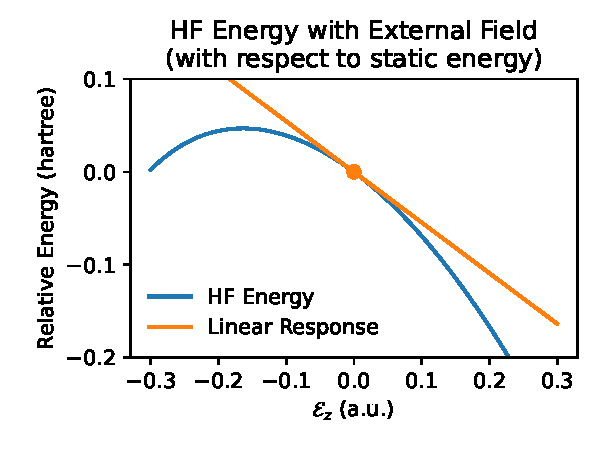
\includegraphics[width=0.5\textwidth]{assets/NumDipole-z.pdf}
    \caption[能量在外加偶极电场下的变化情况]{能量在外场下的变化情况 $E(\symbfscr{E})$。图中的体系是键长 0.9914 \AA、键角 116.10$^\circ$ 的 \ce{NH_3} 体系;$C_3$ 旋转轴与 $z$ 轴重合;计算模型为 HF/6-31G;外场沿 $z$ 轴即外场强度向量 $\symbfscr{E}^\dagger = (0, 0, \mathcal{E}_z)$。蓝色曲线绘制了 $E(\symbfscr{E})$ 关于 $\mathcal{E}_z$ 的函数。橙色曲线绘制了 $\mathcal{E}_z = 0$ 时 $\partial_{\mathcal{E}_z} E$ 的导数值;该导数值等于偶极矩在 $z$ 轴上的分量 $\mu_z$。}
    \label{fig.3.NumDipole-z}
\end{figure}

需要指出,式 (\ref{eq.3.electric-perturbed-hamiltonian}) 所述的 $- \symbfscr{E}^\dagger \bm{r}$ 形式的偶极电场仅仅是外加电场其中一种可能性。若外加电场是 $- \symbfscr{E}^\dagger \bm{Q} \symbfscr{E}$ 的形式,其中
\begin{equation*}
    \bm{Q} =
    \begin{pmatrix}
        x^2 & xy & xz \\
        yx & y^2 & yz \\
        zx & zy & z^2
    \end{pmatrix}
\end{equation*}
那么在该类型的外加电场下,一阶梯度将给出四极矩。电场的其它多级展开还将给出八极矩、十六极矩等等。所有类型的外加电场,在计算化学程序中都表现为对单电子积分与原子核能量的微扰,而对双电子积分、DFA 格点积分能量、原子轨道等部分不产生微扰。本工作着重于极化率,即 $- \symbfscr{E}^\dagger \bm{r}$ 形式的偶极电场下的一阶与二阶梯度,即偶极矩与静态极化率的推导与程序实现;但本文也将用 $\mathbb{A}$ 等记号表示更为一般的外电场;这样能比较容易地拓展到其它形式的外加电场一阶与二阶梯度。

\section{双杂化泛函电性质解析梯度}
\label{sec.3.theory}

本节将在双杂化框架下,讨论电性质导数问题;被求导的性质将以 $\mathbb{A}, \mathbb{B}$ 表示。除非特别指明,一般讨论的是闭壳层情形。不同于分子坐标导数或 GIAO 轨道导数,许多 skeleton 导数对于电性质是零值;因此,这里的讨论不适合推广到所有的梯度问题中。本节不考虑开壳层情形;对于 MP2 型双杂化泛函,将在 \ref{sec.3.program} 节中展开。

\subsection{正交条件、SCF 条件与自洽场泛函对密度矩阵的依赖关系}

在开始梯度理论推演前,先对式 (\ref{eq.3.def.eng-SCF}) 所给出的自洽场计算过程与结果作必要的回顾。这一小节不考虑外场效应。

作为低阶泛函,闭壳层自洽场能量 $E^\textmt{SCF}$ 仅决定于依式 (\ref{eq.3.def.dm-scf-closed-1}, \ref{eq.3.def.dm-scf-closed-2}) 所定义的双占据的密度矩阵 $D_{\mu \nu}$。密度矩阵 $D_{\mu \nu}$ 由分子轨道系数 $C_{\mu i}$ 构成;分子轨道正交归一条件 (后文简称为\textbf{正交条件}) 具体表达为
\begin{empheq}[box=\fbox]{equation}
    \label{eq.3.constraint.ortho}
    S_{pq} = C_{\mu p} S_{\mu \nu} C_{\nu q} = \delta_{pq} \quad \text{(orthogonalization constraint)}
\end{empheq}
原子轨道基的 Fock 矩阵定义为自洽场能量对密度矩阵的导数:
\begin{equation}
    \label{eq.3.def.fock-ao}
    F_{\mu \nu} \coloneq \frac{\partial E^\textmt{SCF}}{\partial D_{\mu \nu}}
\end{equation}
它是自洽场作为变分方法的重要中间量,且为对称矩阵。自洽场能量 $E^\textmt{SCF}$ 对占据轨道 $C_{\mu i}$ 的导数为
\begin{align}
    \label{eq.3.eng-deriv-wrt-coeff}
    \frac{\partial E^\textmt{SCF}}{\partial C_{\mu i}} &= \frac{\partial E^\textmt{SCF}}{\partial D_{\kappa \lambda}} \frac{\partial D_{\kappa \lambda}}{\partial C_{\mu i}}
    = F_{\kappa \lambda} \left( 2 \delta_{\kappa \mu} C_{\lambda i} + 2 \delta_{\lambda \mu} C_{\kappa i} \right) = 4 F_{\mu \nu} C_{\nu i}
\end{align}
占据轨道系数 $C_{\mu i}$ 是通过引入正交条件 (\ref{eq.3.constraint.ortho}) 对 $E^\textmt{SCF}$ 作条件极小值计算得到,同时参考式 (\ref{eq.3.def.C-SCF})。定义对称的 Lagrange 乘子矩阵为 $\varepsilon_{jk}$;下式作为变分方程,对指标 $\nu, j, k$ 求和:
\begin{equation}
    \label{eq.3.hartree-fock-roothaan}
    \frac{\partial}{\partial C_{\mu i}} \big( E^\textmt{SCF} - 2 \varepsilon_{jk} (S_{jk} - \delta_{jk}) \big) = 4 \big( F_{\mu \nu} C_{\nu i} - S_{\mu \nu} C_{\nu j} \varepsilon_{ji} \big) = 0
\end{equation}
若自洽场泛函是 Hartree-Fock,那么上式即 Hartree-Fock-Roothaan 方程\cite{Roothaan-Roothaan.RMP.1951}。

$F_{\mu \nu}$ 作为原子轨道基下的矩阵,秩 $n_\mathrm{orb}$ 明显大于占据轨道数 $n_\mathrm{occ}$;在程序实现中,一般将求取 $n_\mathrm{orb}$ 个分子轨道的系数 $C_{\mu p}$:
\begin{equation}
    \label{eq.3.SCF-working-equation}
    F_{\mu \nu} C_{\nu p} = S_{\mu \nu} C_{\nu q} \varepsilon_{qp} \quad \text{(SCF working equation)}
\end{equation}
但需要注意到,只有占据轨道对自洽场能量产生贡献。关于自洽场对占据布局的限制条件,可以通过对式 (\ref{eq.3.hartree-fock-roothaan}) 等式两边乘以非占轨道系数 $C_{\mu a}$、并对原子轨道指标 $\mu, \nu$ 求和结果所体现:
\begin{equation*}
    4 (C_{\mu a} F_{\mu \nu} C_{\nu i} - C_{\mu a} S_{\mu \nu} C_{\nu j} \varepsilon_{ji}) = 4 (F_{ai} - S_{aj} \varepsilon_{ji}) = 0
\end{equation*}
或更简洁地,Fock 矩阵在分子轨道基下是分块对角化的:
\begin{empheq}[box=\fbox]{equation}
    \label{eq.3.constraint.SCF}
    F_{ai} = 0 \quad \text{(SCF constraint)}
\end{empheq}
上式在后文称为 \textbf{SCF 条件};推演过程利用了正交条件 (\ref{eq.3.constraint.ortho}) 所给出的 $S_{aj} = 0$ (占据轨道与非占轨道指标不可能一致)。

正交条件与 SCF 条件是梯度推演中,所有必要的额外限制条件。

最后,为了后面推导的便利,这里引入 A 张量的前导张量 $\tilde A_{\mu \nu, \kappa \lambda}$ (Fock 轨道响应张量) 作为 Fock 矩阵对密度矩阵的导数量:
\begin{equation}
    \label{eq.3.def.Auvkl-pre}
    \tilde A_{\mu \nu, \kappa \lambda} \coloneq \frac{\partial^2 E^\textmt{SCF}}{\partial D_{\mu \nu} \partial D_{\kappa \lambda}} = \frac{\partial F_{\mu \nu}}{\partial D_{\kappa \lambda}}
\end{equation}
该张量通常具有 4 重对称性:
\begin{equation*}
    \tilde A_{\mu \nu, \kappa \lambda} = \tilde A_{\kappa \lambda, \mu \nu} = \tilde A_{\nu \mu, \lambda \kappa} = \tilde A_{\lambda \kappa, \nu \mu}
\end{equation*}
但需要指出,若交换能 $E_\textmt{x}^\textmt{exact}$ (或不同于 $\hat g$ 的算符所贡献的 ERI 交换能) 对能量项有贡献,那么该张量不是 8 重对称性的 (即不满足 $\tilde A_{\mu \nu, \kappa \lambda} = \tilde A_{\mu \nu, \lambda \kappa}$)。出于便利,我们将定义下述 8 重对称性的张量 $A_{\mu \nu, \kappa \lambda}$,该张量称为 A 张量:
\begin{equation}
    \label{eq.3.def.Auvkl}
    A_{\mu \nu, \kappa \lambda} \coloneq 2 \left( \tilde A_{\mu \nu, \kappa \lambda} + \tilde A_{\mu \nu, \lambda \kappa} \right)
\end{equation}
上式定义中的 2 倍,是出于闭壳层情形下,下述表达式方便而给出:
\begin{align}
    \frac{\partial F_{\mu \nu}}{\partial C_{\kappa i}} &= \frac{\partial F_{\mu \nu}}{\partial D_{\eta \lambda}} \frac{\partial D_{\eta \lambda}}{\partial C_{\kappa i}}
    = 2 \tilde A_{\mu \nu, \eta \kappa} \left( \delta_{\eta \kappa} C_{\lambda i} + \delta_{\lambda \kappa} C_{\eta i} \right) \notag\\
    &= 2 \left( \tilde A_{\mu \nu, \kappa \lambda} + \tilde A_{\mu \nu, \lambda \kappa} \right) C_{\lambda i} \notag\\
    &= A_{\mu \nu, \kappa \lambda} C_{\lambda i} = A_{\mu \nu, \kappa i}
\end{align}
上式的第三个等号利用了被求和指标 $\eta, \lambda$ 的轮换。

\subsection{一阶梯度:轨道系数随外场的变化}

自洽场泛函 $E^\textmt{SCF}$ 与能量泛函 $E^\textmt{DH}$ 的运算共用同一轨道系数 $C_{\mu i}$。这一小节进一步讨论正交条件、SCF 条件在外场微扰 $\mathbb{A}$ 下的响应,并籍此给出描述轨道系数在外场微扰下变化的 U 矩阵 $U_{pq}^\mathbb{A}$\footnote{式 (\ref{eq.3.def.U}) 中 U 矩阵的定义并非在等式左边。利用正交条件 (\ref{eq.3.constraint.ortho}),可知
\begin{equation}
    U_{pq}^\mathbb{A} \coloneq C_{\mu p} S_{\mu \nu} \partial_\mathbb{A} C_{\nu q}
\end{equation}
上述定义式与导出式 (\ref{eq.3.def.U}) 是等价的。出于推演方便,我们仅使用导出式 (\ref{eq.3.def.U})。}:
\begin{empheq}[box=\fbox]{equation}
    \label{eq.3.def.U}
    \partial_\mathbb{A} C_{\mu q} = C_{\mu p} U_{pq}^\mathbb{A}
\end{empheq}
这一小节首先确定 U 矩阵在占据-非占部分 $U_{ai}^\mathbb{A}$ 的表达式。其余部分在后一小节详细描述。

对正交条件 (\ref{eq.3.constraint.ortho}) 作性质 $\mathbb{A}$ 的导数:
\begin{align*}
    \partial_\mathbb{A} S_{pq} &= \partial_\mathbb{A} C_{\mu p} S_{\mu \nu} C_{\nu q} + C_{\mu p} \partial_\mathbb{A} S_{\mu \nu} C_{\nu q} + C_{\mu p} S_{\mu \nu} \partial_\mathbb{A} C_{\nu q} \notag\\
    &= S_{mq} U_{mp}^\mathbb{A} + S_{pm} U_{mq}^\mathbb{A} = U_{pq}^\mathbb{A} + U_{qp}^\mathbb{A} = 0
\end{align*}
或更简洁地,
\begin{empheq}[box=\fbox]{equation}
    \label{eq.3.collary.ortho}
    U_{pq}^\mathbb{A} + U_{qp}^\mathbb{A} = 0 \quad \text{(corollary of orthogonalization constraint)}
\end{empheq}
上述推导过程中利用到电性质微扰下基轨道没有变化,因此 $\partial_\mathbb{A} S_{\mu \nu} = 0$。上述结论表明,U 矩阵在电性质导数下是反对称的\footnote{需要指出,对于其它性质梯度,由于 $\partial_\mathbb{A} S_{\mu \nu}$ 未必是零,因此 U 矩阵一般来说未必是反对称或反厄米的。后文将有许多结论只能用于电性质微扰,而无法简单地扩展到所有情形。在本工作中,不会一一列举所有无法扩展的情形。}。

进而将对 SCF 条件 (\ref{eq.3.constraint.SCF}) 的等式两边作性质 $\mathbb{A}$ 的导数。但在考虑 $\partial_\mathbb{A} F_{ai}$ 前,我们先考虑更一般的原子轨道基下 Fock 矩阵的导数:
\begin{equation}
    \label{eq.3.deduct.pd-Fuv}
    \partial_\mathbb{A} F_{\mu \nu} = \partial_\mathbb{A}^\mathrm{S} F_{\mu \nu} + \partial_\mathbb{A}^\mathrm{U} F_{\mu \nu}
    = F_{\mu \nu}^\mathbb{A} + \frac{\partial F_{\mu \nu}}{\partial C_{\kappa i}} \partial_\mathbb{A} C_{\kappa i}= F_{\mu \nu}^\mathbb{A} + A_{\mu \nu, mi} U_{mi}^\mathbb{A}
\end{equation}
其中,$F_{\mu \nu}^\mathbb{A} \coloneq \partial_\mathbb{A}^\mathrm{S} F_{\mu \nu}$ 定义为不受密度矩阵扰动、而仅受外场扰动产生变化的 skeleton 导数部分。作为特例,对于外加偶极电场而言,从式 (\ref{eq.3.def.huv-with-perturb}) 附近的讨论出发,仅有单电子算符部分产生贡献:
\begin{align}
    \label{eq.3.def.sleketon-huv}
    F_{\mu \nu}^{\mathcal{E}_t} = h_{\mu \nu}^{\mathcal{E}_t} &\coloneq \partial_{\mathcal{E}_t} h_{\mu \nu} = h_{\mu \nu}^t \\
    F_{pq}^{\mathcal{E}_t} = h_{pq}^{\mathcal{E}_t} &= C_{\mu p} F_{\mu \nu}^{\mathcal{E}_t} C_{\nu q}
\end{align}
对于多级展开的外电场也是类似的;我们将在所有电性质导数问题中,假定 $F_{\mu \nu}^\mathbb{A} = h_{\mu \nu}^\mathbb{A}$ 与 $F_{pq}^\mathbb{A} = h_{pq}^\mathbb{A}$。

得到原子轨道基 Fock 矩阵导数 $\partial_\mathbb{A} F_{\mu \nu}$ 后,分子轨道下的导数可以顺势得到:
\begin{align}
    \label{eq.3.pd-Fpq-0}
    \partial_\mathbb{A} F_{pq} &= F_{mq} U_{mp}^\mathbb{A} + F_{pm} U_{mq}^\mathbb{A} + C_{\mu p} \partial_\mathbb{A} F_{\mu \nu} C_{\nu q} \notag\\
    &= F_{mq} U_{mp}^\mathbb{A} + F_{pm} U_{mq}^\mathbb{A} + F_{pq}^\mathbb{A} + A_{pq, mj} U_{mj}^\mathbb{A}
\end{align}
上式在二阶梯度求取、以及 MP2 的激发张量导数计算上经常用到;但在这一小节,我们只对其非占-占据部分感兴趣。对 SCF 条件 (\ref{eq.3.constraint.SCF}) 的两边求导,得到
\begin{align}
    \label{eq.3.Fai-deriv-without-canonical}
    \partial_\mathbb{A} F_{ai} &= F_{mi} U_{ma}^\mathbb{A} + F_{am} U_{mi}^\mathbb{A} + F_{ai}^\mathbb{A} + A_{ai, mj} U_{mj}^\mathbb{A} = 0
\end{align}
该式还可以简化。首先,SCF 条件要求分子轨道基下 Fock 占据-非占部分为零;这意味着上式第一项指标 $m$ 对非占轨道求和、第二项指标 $m$ 对占据轨道求和的部分不产生贡献;即前两项的贡献可以写为
\begin{align*}
    \partial_\mathbb{A} F_{ai}
    \leftarrow F_{mi} U_{ma}^\mathbb{A} + F_{am} U_{mi}^\mathbb{A}
    = F_{ij} U_{ja}^\mathbb{A} + F_{ab} U_{bi}^\mathbb{A} = - F_{ij} U_{aj}^\mathbb{A} + F_{ab} U_{bi}^\mathbb{A}
\end{align*}
同时,利用 U 矩阵的反对称性和 A 张量的对称性,最后一项 $A_{ai, mj} U_{mj}^\mathbb{A}$ 中 $m$ 仅对占据轨道求和为零,
\begin{align*}
    \partial_\mathbb{A} F_{ai} \leftarrow A_{ai, kj} U_{kj}^\mathbb{A} = \frac{1}{2} \left( A_{ai, kj} U_{kj}^\mathbb{A} + A_{ai, jk} U_{kj}^\mathbb{A} \right) = \frac{1}{2} \left( A_{ai, kj} U_{kj}^\mathbb{A} + A_{ai, kj} U_{jk}^\mathbb{A} \right) = 0
\end{align*}
因而 SCF 条件 (\ref{eq.3.constraint.SCF}) 两侧求导后的最终结论可以写为
\begin{empheq}[box=\fbox]{equation}
    \label{eq.3.pd-Fai-0}
    \partial_\mathbb{A} F_{ai} = - F_{ij} U_{aj}^\mathbb{A} + F_{ab} U_{bi}^\mathbb{A} + F_{ai}^\mathbb{A} + A_{ai, bj} U_{bj}^\mathbb{A} = 0
    \quad \text{(corollary of SCF constraint)}
\end{empheq}

若引入\textbf{正则 SCF 条件},即 Fock 矩阵是对角化的:
\begin{empheq}[box=\fbox]{equation}
    \label{eq.3.constraint.canonical-SCF}
    F_{pq} = \varepsilon_p \delta_{pq} \quad \text{(canonical SCF constraint)}
\end{empheq}
那么,式 (\ref{eq.3.pd-Fai-0}) 可以写为
\begin{equation}
    \label{eq.3.intermediate-pd-Fai-1}
    \partial_\mathbb{A} F_{ai} = (\varepsilon_a - \varepsilon_i) U_{ai}^\mathbb{A} + F_{ai}^\mathbb{A} + A_{ai, mj} U_{mj}^\mathbb{A} = 0
\end{equation}
对上式整理,得到电性质导数下的 CP-SCF 方程
\begin{empheq}[box=\fbox]{align}
    \label{eq.3.CP-SCF}
    F_{ai}^\mathbb{A} &= - (\varepsilon_a - \varepsilon_i) U_{ai}^\mathbb{A} - A_{ai, bj} U_{bj}^\mathbb{A} \notag\\
    &= - \left( (\varepsilon_a - \varepsilon_i) \delta_{ai, bj} + A_{ai, bj} \right) U_{bj}^\mathbb{A} \quad \text{(CP-SCF)}
\end{empheq}
通过该方程可以求得 U 矩阵的非占-占据部分 $U_{ai}^\mathbb{A}$。其耦合微扰的意义是,不仅 Hamilton 算符受外场扰动、自洽场波函数也因 Hamilton 算符的微扰而随之产生变化;CP-SCF 方程所给出的 U 矩阵确定了轨道系数 (作为描述自洽场波函数的参数) 是如何随外场发生扰动的。

\subsection{一阶梯度:U 矩阵占据-占据和非占-非占部分}
\label{sec.3.Uia-Uai}

对于自洽场泛函 $E^\textmt{SCF}$ 求得轨道系数 $C_{\mu p}$ 的过程,只有正交条件 $S_{pq} = \delta_{pq}$ 与 SCF 条件 $F_{ai} = 0$ 是必须满足的条件。这意味着
\begin{itemize}[nosep]
    \item 在外场微扰下,正交条件与 SCF 条件也需要满足,这已经在式 (\ref{eq.3.collary.ortho}, \ref{eq.3.pd-Fai-0}) 附近的讨论有所展开;
    \item 正则 SCF 条件 (\ref{eq.3.constraint.canonical-SCF}) 不是必要的,这同时意味着轨道系数 $C_{\mu p}$ 的选取并非是唯一的;通常只是为公式推演的便利与程序实现的高效,而引入了正则 SCF 条件。
\end{itemize}
外场 $\mathbb{A}$ 对轨道系数的扰动即是 U 矩阵。上一小节的推演,在仅仅使用正交条件与 SCF 条件时,作为结论的式 (\ref{eq.3.collary.ortho}, \ref{eq.3.pd-Fai-0}) 表明 U 矩阵仅仅在占据-非占部分 $U_{ai}^\mathbb{A}$ 有非平凡的贡献与确定的定义;而对占据-占据 $U_{ij}^\mathbb{A}$ 和非占-非占 $U_{ab}^\mathbb{A}$ 部分只有反对称的限制,没有确定的定义。

不失一般性,下面的讨论在没有外场微扰的情形下,仍然引入正则 SCF 条件 (\ref{eq.3.constraint.canonical-SCF});但存在外场微扰的情形改下,Fock 矩阵在占据-占据或非占-非占部分的导数未必是对角阵:
\begin{equation}
    \label{eq.3.weak-canonical-SCF}
    \partial_\mathbb{A} F_{ij} \not \equiv 0 \quad (i \neq j); \quad \partial_\mathbb{A} F_{ab} \not \equiv 0 \quad (a \neq b) \quad \text{(weak canonical SCF)}
\end{equation}
对于这种情形,我们称之为\textbf{弱的正则 SCF 条件}。

下面先讨论占据-占据部分。弱的正则 SCF 条件下,利用 Fock 矩阵为对角阵、以及 U 矩阵反对称性质,
\begin{align}
    \label{eq.3.pdA-Fij-temp}
    \partial_\mathbb{A} F_{ij} &= F_{im} U_{mj}^\mathbb{A} + F_{mj} U_{mi}^\mathbb{A} + F_{ij}^\mathbb{A} + A_{ij, mk} U_{mk}^\mathbb{A} \notag\\
    &= (\varepsilon_i - \varepsilon_j) U_{ij}^\mathbb{A} + F_{ij}^\mathbb{A} + A_{ij, bk} U_{bk}^\mathbb{A}
\end{align}
通过 CP-SCF 方程 (\ref{eq.3.CP-SCF}) 可以求得 $U_{bj}^\mathbb{A}$;同时注意到 U 矩阵的反对称性 (\ref{eq.3.collary.ortho}) 即 U 矩阵对角元为零,从而上式整理为
\begin{equation}
    \label{eq.3.Uij-weak-canonical}
    U_{ij}^\mathbb{A} = 
    \begin{cases}
    \displaystyle
    - \frac{F_{ij}^\mathbb{A} + A_{ij, bk} U_{bk}^\mathbb{A} - \partial_\mathbb{A} F_{ij}}{\varepsilon_i - \varepsilon_j} & (i \neq j) \\
    0 & (i = j)
    \end{cases}
\end{equation}

若 Fock 矩阵导数也是对角矩阵,即 $\partial_\mathbb{A} F_{ij} = \delta_{ij} \partial_\mathbb{A} \varepsilon_i$,那么我们称其为\textbf{强的正则 SCF 条件}。代入该条件到式 (\ref{eq.3.Uij-weak-canonical}, \ref{eq.3.pdA-Fij-temp}),
\begin{alignat}{10}
    \label{eq.3.unstable-Uij}
    U_{ij}^\mathbb{A} &= - \frac{F_{ij}^\mathbb{A} + A_{ij, bk} U_{bk}^\mathbb{A}}{\varepsilon_i - \varepsilon_j} &&\quad \left( i \neq j, \, \text{strong canonical SCF}\right) \\
    \label{eq.3.unstable-pdA-eo}
    \partial_\mathbb{A} \varepsilon_i &= F_{ij}^\mathbb{A} + A_{ij, bk} U_{bk}^\mathbb{A} &&\quad \text{(strong canonical SCF)}
\end{alignat}
上式的分子一般非零,而分母 $\varepsilon_i - \varepsilon_j$ 则有可能接近或等于零;举例而言,甲烷分子的最高能级占据轨道为 $T_d$ 不可约表示,即三重简并,因此存在 $i \neq j$ 且 $\varepsilon_i - \varepsilon_j = 0$ 的情形,从而将 $U_{ij}^\mathbb{A}$ 推向无穷大。这在程序实现中将导致严重的数值误差,因此一般来说不适合引入强的正则 SCF 条件。方才分析的是 Fock 矩阵导数占据-占据部分 $\partial_\mathbb{A} F_{ij}$;对于非占-非占部分 $\partial_\mathbb{A} F_{ab}$ 也有类似的结论。

但也需要指出,对于 MP2 的激发张量梯度 $\partial_\mathbb{A} t_{ij}^{ab}$ (\ref{eq.3.pdA-tijab}),其存在贡献项:
\begin{equation*}
    \partial_\mathbb{A} t_{ij}^{ab} \leftarrow - \partial_\mathbb{A} F_{ca} t_{ij}^{cb}
\end{equation*}
若 $\partial_\mathbb{A} F_{ij}$ 与 $\partial_\mathbb{A} F_{ab}$ 是对角矩阵,那么该项计算复杂度可以从 $O(n_\mathrm{prop} n_\mathrm{occ}^2 n_\mathrm{vir}^3) \sim O(N^5)$ 降至 $O(n_\mathrm{prop} n_\mathrm{occ}^2 n_\mathrm{vir}^2) \sim O(N^4)$;即使用强正则 SCF 条件可以付出数值误差的代价、换取计算效率。

若仅考虑弱的正则 SCF 条件 (\ref{eq.3.weak-canonical-SCF}),那么 $U_{ij}^\mathbb{A}$ 与 $U_{ab}^\mathbb{A}$ 只需要满足条件 (\ref{eq.3.collary.ortho}) 即可;其最简单的定义方式是置零:
\begin{empheq}[box=\fbox]{equation}
    \label{eq.3.Uij-Uab-zero}
    U_{ij}^\mathbb{A} = U_{ab}^\mathbb{A} = 0 \quad \text{(definition of program implementation)}
\end{empheq}
本工作的程序也按上式实现。依上述定义,Fock 矩阵的导数在非对角元上未必为零;以占据-占据部分为例,
\begin{equation}
    \label{eq.3.pd-Fpq-not-diagonal}
    \begin{alignedat}{10}
        \partial_\mathbb{A} F_{ij} &= F_{ij}^\mathbb{A} + A_{ij, ck} U_{ck}^\mathbb{A} \not \equiv 0 && \quad (\forall i, j \in \mathrm{occ}) \\
        \partial_\mathbb{A} F_{ab} &= F_{ab}^\mathbb{A} + A_{ab, ck} U_{ck}^\mathbb{A} \not \equiv 0 && \quad (\forall a, b \in \mathrm{vir}) \\
    \end{alignedat}
    \quad (\text{(\ref{eq.3.Uij-Uab-zero}) satisfied})
\end{equation}
如此可以避免 U 矩阵的数值不稳定性;但对于 MP2 的激发张量梯度 $\partial_\mathbb{A} t_{ij}^{ab}$ (\ref{eq.3.pdA-tijab}) 的计算,其复杂度将是 $O(N^5)$。

上述两种情形 (\ref{eq.3.unstable-Uij}, \ref{eq.3.Uij-Uab-zero}) 在计算 (\ref{eq.3.pdA-tijab}) 时,或者存在潜在的数值误差、或者计算复杂度较高。一种折中方案由 Stoychev 等人在程序中实现。对于简并或近简并的一部分轨道,定义非对角的 $\partial_\mathbb{A} F_{pq}$;而剩余下来不存在简并情况的轨道,它们构成的 $\partial_\mathbb{A} F_{pq}$ 仍然是对角的。在这种方案下由于三维空间的最大不可约表示是三维,而 $3 \times 3$ 矩阵的元素数是长度为 3 向量数的 3 倍,因此 FLOPs 不会超过 3 倍于 $n_\mathrm{prop} n_\mathrm{occ}^2 n_\mathrm{vir}^2$ 的乘积累加运算\cite{Stoychev-Neese.JCTC.2018}。但这种方案并非简单的张量乘积,程序实现上会引入一定的复杂性;在我们目前的公开程序中,没有实现上述折中方案。

若不加说明,后文的讨论将基于式 (\ref{eq.3.Uij-Uab-zero}) 的弱正则 SCF 条件。

\subsection{一阶梯度:能量泛函导数}

这一小节讨论能量泛函 $E^\textmt{DH}$ 在性质 $\mathbb{A}$ 微扰下的导数。

DH 总能量的全导数可以分为 skeleton 部分与对轨道系数的导数两部分:
\begin{equation}
    \label{eq.3.def.pdA-DH-0}
    \partial_\mathbb{A} E^\textmt{DH} = \partial_\mathbb{A}^\mathrm{S} E^\textmt{DH} + \frac{\partial E^\textmt{DH}}{\partial C_{\mu q}} \partial_\mathbb{A} C_{\mu q}
\end{equation}
对于轨道系数导数部分,我们作更多讨论。定义 DH 广义 Fock 矩阵为
\begin{equation}
    \label{eq.3.def.generalized-fock}
    \symscr{F}_{pq}^\textmt{DH} \coloneq C_{\mu p} \frac{\partial E^\textmt{DH}}{\partial C_{\mu q}}
\end{equation}
该矩阵的性质是
\begin{itemize}[nosep]
    \item 若 $E^\textmt{DH} = E^\textmt{SCF}$,则广义 Fock 矩阵的占据-占据部分 $\symscr{F}_{ij}^\textmt{DH}$ 退化到自洽场 Fock 矩阵 $F_{ij}$;但非占-非占部分 $\symscr{F}_{ab}^\textmt{DH}$ 数值上是零,因非占轨道对自洽场能量没有影响;
    \item 对于本工作考虑的 DH,广义 Fock 矩阵一般不是对角化的、对称的;非占-占据或占据-非占部分也未必为零\footnote{并非所有双杂化泛函 Fock 矩阵不是对角矩阵。轨道优化 (orbital-optimized) MP2 或双杂化泛函,其变分条件即是广义 Fock 矩阵对角化\cite{Bozkaya-Sherrill.JCP.2011}。轨道优化泛函尽管在性质计算上有一定的优势\cite{Hait-Head-Gordon.JCP.2018},但其计算代价很大。这类型方法需要多次迭代地计算广义 Fock 矩阵、单步 MP2 相关能因非正则 SCF 的缘故也需迭代计算得到,且广义 Fock 矩阵计算消耗一般不小于 MP2 相关能计算。}。
\end{itemize}
进而引入 DH Lagrangian 为广义 Fock 反对称化矩阵\footnote{在本文中,Lagrangian 通过广义 Fock 矩阵所定义。但一般来说,Lagrangian 应当通过轨道或密度在旋转矩阵下的导数定义\cite{Helgaker-Jorgensen.Wiley.2013};因此,应当认为广义 Fock 反对称化矩阵的结果等于 Lagrangian,而非后者为前者所定义。但比较严格地引入 Lagrangian 将占用一定的篇幅。}:
\begin{equation}
    \label{eq.3.def.lagrangian}
    L_{pq}^\textmt{DH} \coloneq \symscr{F}_{pq}^\textmt{DH} - \symscr{F}_{qp}^\textmt{DH}
\end{equation}
注意到对于电性质而言,U 矩阵可以定义为 (\ref{eq.3.Uij-Uab-zero});因此,
\begin{align}
    \label{eq.3.derivation-contrib-Lai-to-engderiv}
    \partial_\mathbb{A} E^\textmt{DH} &\leftarrow \frac{\partial E^\textmt{DH}}{\partial C_{\mu q}} \frac{\partial C_{\mu q}}{\partial \mathbb{A}} = \symscr{F}_{pq}^\textmt{DH} U_{pq}^\mathbb{A} \notag\\
    &= \symscr{F}_{ai}^\textmt{DH} U_{ai}^\mathbb{A} + \symscr{F}_{ia}^\textmt{DH} U_{ia}^\mathbb{A} + \symscr{F}_{ij}^\textmt{DH} U_{ij}^\mathbb{A} + \symscr{F}_{ab}^\textmt{DH} U_{ab}^\mathbb{A} \notag\\
    &= (\symscr{F}_{ai}^\textmt{DH} - \symscr{F}_{ia}^\textmt{DH}) U_{ai}^\mathbb{A} + 0 = L_{ai}^\textmt{DH} U_{ai}^\mathbb{A}
\end{align}
特别地,对于自洽场方法,$L_{ai}^\textmt{SCF} = 0$。从而,电性质微扰下 DH 一阶泛函能量导数可以写为
\begin{empheq}[box=\fbox]{equation}
    \label{eq.3.derivation-dh-energy-deriv-abstract}
    \partial_\mathbb{A} E^\textmt{DH} = \partial_\mathbb{A}^\mathrm{S} E^\textmt{DH} + L_{ai}^\textmt{DH} U_{ai}^\mathbb{A}
\end{empheq}

正因为 DH 包含了公式形式复杂的 $E_\textmt{c}^\textmt{PT} [\mathbf{C}]$、其 Lagrangian 一般地非零即 $L_{ai}^\textmt{DH} \not \equiv 0$,从而 DH 的梯度理论相比之自洽场而言要复杂不少。

\subsection{一阶梯度:约化密度矩阵}
\label{sec.3.resp-den}

本工作区分约化密度 $D_{pq}^{\textmt{DH}, \textmt{RDM}}$ (\ref{eq.3.collary.rdm-definition}) 与弛豫密度 $D_{pq}^{\textmt{DH}}$ 为不同的量。

约化密度与电性质 skeleton 导数有直接的联系。这里先以 CI 波函数 $| \Psi^\textmt{CI} \rangle$ 开始讨论,随后引申到 DH 约化密度。本小节与下一小节参考 Trucks 等的工作\cite{Trucks-Bartlett.CPL.1988}。

CI 的 (一阶) 约化密度在分子轨道基下,通过二次量子化算符,一般定义为
\begin{equation}
    \label{eq.3.def.rdm-ci}
    D_{qp}^{\textmt{CI},\textmt{RDM}} \coloneq \frac{\langle \Psi^\textmt{CI} | a_p^\dagger a_q | \Psi^\textmt{CI} \rangle}{\langle \Psi^\textmt{CI} | \Psi^\textmt{CI} \rangle}
\end{equation}
约化密度矩阵的意义是,对于任意的单电子算符 $\hat o = o_{pq} a_p^\dagger a_q$,其期望值总是可以写为约化密度矩阵 $D_{qp}^{\textmt{CI},\textmt{RDM}}$ 与算符矩阵表示 $o_{pq}$ 的乘积:
\begin{equation*}
    \langle \hat o \rangle = \frac{\langle \Psi^\textmt{CI} | \hat o | \Psi^\textmt{CI} \rangle}{\langle \Psi^\textmt{CI} | \Psi^\textmt{CI} \rangle} = o_{pq} D_{qp}^{\textmt{CI},\textmt{RDM}}
\end{equation*}
注意到 $(a_p^\dagger a_q)^\dagger = a_q^\dagger a_p$,因此 $D_{qp}^{\textmt{CI},\textmt{RDM}}$ 是复共轭的。由于本工作仅考虑实数范围内的问题,因此可以认为约化密度矩阵是对称的。

现在考虑 CI 波函数的电性质 skeleton 导数问题。对于 Hamilton 算符 $\hat H$,电子所引起的能量效应中,电性质仅对单电子算符 $\hat h = \hat T + \hat V_\mathrm{ext}$ 中的外势 $\hat V_\mathrm{ext}$ 有微扰贡献:
\begin{equation}
    \partial_\mathbb{A}^\mathrm{S} \hat H = \partial_\mathbb{A}^\mathrm{S} \hat h + \partial_\mathbb{A} \hat V_\textmt{non-elec} = h_{pq}^\mathbb{A} a_p^\dagger a_q + \partial_\mathbb{A} \hat V_\textmt{non-elec}
\end{equation}
依 Hellmann-Feynman 定理,算符期望的 skeleton 导数等于 skeleton 导数下算符的期望:
\begin{align}
    \partial_\mathbb{A}^\mathrm{S} E^\textmt{CI} &= \partial_\mathbb{A}^\mathrm{S} \langle \hat H \rangle = \langle \partial_\mathbb{A}^\mathrm{S} \hat H \rangle = \langle \partial_\mathbb{A}^\mathrm{S} \hat h \rangle + \partial_\mathbb{A} E^\textmt{non-elec} \notag\\
    &= h_{pq}^\mathbb{A} D_{pq}^{\textmt{CI}, \textmt{RDM}} + \partial_\mathbb{A} E^\textmt{non-elec}
\end{align}

但作为常见的 DH 能量贡献项,MP2 相关能或其它形式的相关能,在定义约化密度的问题上存在困难。MP2 方法的波函数并非是对 $\hat H$ 变分极小的,因此 Hellmann-Feynman 定理失效,从而 MP2 方法的约化密度矩阵不能通过与 CI 相同的方式 (\ref{eq.3.def.rdm-ci}) 所定义\footnote{
    作为波函数方法,MP2 相关能可以通过 Hylleraas 泛函给出\cite{Hylleraas-Hylleraas.ZP.1930, Pulay-Saeboe.TCA.1986}:
    \begin{equation*}
    E_\textmt{c}^\textmt{(2)} = \min_{\Psi^{(1)}} \left( 2 \langle \Psi^\textmt{(1)} | \hat H - E^\textmt{0} | \Phi^\textmt{0} \rangle - \langle \Psi^\textmt{(1)} | \hat F - E^\textmt{0} | \Psi^\textmt{(1)} \rangle \right)
    \end{equation*}
    这里的 $\Phi^\textmt{0}$ 是 Hartree-Fock 行列式,$E^\textmt{0} = \langle \Phi^\textmt{0} | \hat F | \Phi^\textmt{0} \rangle$ 为零阶能量 (占据轨道能之和),$\Psi^\textmt{(1)}$ 是 MP2 相关波函数。上式对 $\Psi^\textmt{(1)}$ 取变分极小,因此尽管 MP2 并非变分方法,但 Hellmann-Feynman 定理适用于上式。又由于 Brillouin 定理,$\Psi^\textmt{(1)}$ 只有二次激发项贡献、没有单次激发项,故对于任何单电子算符 $\hat o$ 总有 $\langle \Psi^\textmt{(1)} | \hat o | \Phi^\textmt{0} \rangle = 0$。故 MP2 相关部分对约化密度矩阵贡献是
    \begin{equation}
    D_{pq}^{\textmt{(2)},\textmt{RDM}} = - \langle \Psi^\textmt{(1)} | a_p^\dagger a_q | \Psi^\textmt{(1)} \rangle
    \end{equation}
    上述推导基于自旋轨道;应当可以验证,在开壳层或闭壳层的限制下,通过 $\partial_\mathbb{A}^\mathrm{S} E \leftarrow h_{pq}^\mathbb{A} D_{pq}^\textmt{RDM}$ 给出的约化密度矩阵,与通过二次量子化算符下给出的约化密度矩阵是一致的。闭壳层 $D_{pq}^{\textmt{(2)},\textmt{RDM}}$ 的具体表达式、以及其与 skeleton 导数的联系,在 \ref{sec.3.skeleton} 小节给出。
}。但我们注意到,若能量的电性质 skeleton 导数的电子效应部分可以写为下述矩阵乘积与非电子效应导数之和:
\begin{empheq}[box=\fbox]{equation}
    \label{eq.3.collary.rdm-definition}
    \partial_\mathbb{A}^\mathrm{S} E \eqcolon h_{pq}^\mathbb{A} D_{pq}^\textmt{RDM} + \partial_\mathbb{A} E^\textmt{non-elec} \quad \text{(electric property)}
\end{empheq}
那么就可以从 skeleton 导数 $\partial_\mathbb{A}^\mathrm{S} E$ 推出约化密度矩阵 $D_{pq}^\textmt{RDM}$\footnote{
    但注意到,若是其它性质,譬如原子核导数问题,skeleton 导数对基组本身产生扰动,因而式 (\ref{eq.3.def.eng-DH}) 所定义的能量项的每一项都有 skeleton 导数的贡献;这将导致表达式较为复杂,即单电子 skeleton 导数 $\partial_\mathbb{A}^\mathrm{S} E \leftarrow h_{pq}^\mathbb{A} D_{pq}^\textmt{RDM}$ 只是众多原子核导数贡献的其中一个电子效应项。因此,通过 skeleton 导数给出约化密度,只能在电性质梯度下、或其它仅对单电子算符产生微扰的性质下,方能成立。
}。该约化密度矩阵的定义不仅适用于 MP2 等非变分的后自洽场方法,也适用于双杂化泛函。我们记 DH 的约化密度为 $D_{pq}^{\textmt{DH}, \textmt{RDM}}$。

\subsection{一阶梯度:Z-Vector 方法与弛豫密度}
\label{sec.3.Z-vector}

式 (\ref{eq.3.derivation-dh-energy-deriv-abstract}) 中 $\partial_\mathbb{A} E^\textmt{DH}$ 求取的第二项可以进一步整理。该整理过程对二阶梯度的推导也是重要的。

注意到 $U_{ai}^\mathbb{A}$ 有三个指标,其张量维度是 $(n_\mathrm{prop}, n_\mathrm{vir}, n_\mathrm{occ})$。$U_{ai}^\mathbb{A}$ 的求取是通过 CP-SCF 方程 (\ref{eq.3.CP-SCF}) 给出,其计算量在不预先存储 A 张量 $A_{ia, jb}$ 时较大,是有效率优化价值的计算过程。

Handy 与 Schaefer III 指出\cite{Handy-Schaefer.JCP.1984},对于一阶梯度,若 Lagrangian 为 $L_{ai}$,则不需要求取 $(n_\mathrm{prop}, n_\mathrm{vir}, n_\mathrm{occ})$ 维度的 U 矩阵 $U_{ai}^\mathbb{A}$,而只需要求取 $(n_\mathrm{vir}, n_\mathrm{occ})$ 维度的 Z 矩阵 $Z_{ai}$:
\begin{empheq}[box=\fbox]{equation}
    \label{eq.3.Z-vector}
    - (\varepsilon_a - \varepsilon_i) Z_{ai} - A_{ai, bj} Z_{bj} = L_{ai} \quad \text{(definition of } Z_{ai} \text{)}
\end{empheq}
理想情况下,相比于求解 CP-SCF 方程 (\ref{eq.3.CP-SCF}) 得到 $U_{ai}^\mathbb{A}$,通过上式求解 $Z_{ai}^\mathbb{A}$ 的计算耗时要少 $n_\mathrm{prop}$ 倍。在本工作中,该方程称为 Z-Vector 方程。那么 Lagrangian 对能量的贡献可以化为
\begin{empheq}[box=\fbox]{equation}
    \label{eq.3.Z-vector-contrib-to-eng-deriv}
    \partial_\mathbb{A} E \leftarrow L_{ai} U_{ai}^\mathbb{A} = Z_{ai} F_{ai}^\mathbb{A}
\end{empheq}

这里有必要回顾 Z-Vector 方法,因为其推演过程将对二阶梯度的计算有所帮助。为方便起见,定义
\begin{equation}
    \label{eq.3.def.scrA}
    \symscr{A}_{ai,bj} \coloneq - \left( (\varepsilon_a - \varepsilon_i) \delta_{ai, bj} + A_{ai, bj} \right)
\end{equation}
现在将指标 $ai$ 和 $bj$ 看作联合指标 (即将 $Z_{ai}$ 视作关于指标 $ai$ 的一维向量 $\mathbf{Z}$、将 $\symscr{A}_{ai, bj}$ 视作关于指标 $ai$、$bj$ 的二维矩阵 $\symbfscr{A}$)。那么,CP-SCF 方程 (\ref{eq.3.CP-SCF}) 与 Z-Vector 方程 (\ref{eq.3.Z-vector}) 分别写为
\begin{align}
    \label{eq.3.CP-SCF-matrix-form}
    \symbfscr{A} \mathbf{U}^\mathbb{A} &= \mathbf{F}^\mathbb{A} \\
    \label{eq.3.Z-Vector-matrix-form}
    \symbfscr{A} \mathbf{Z} &= \mathbf{L}
\end{align}
从而,U 矩阵可以表示为 $\mathbf{U}^\mathbb{A} = \symbfscr{A}^{-1} \mathbf{F}^\mathbb{A}$,Z 矩阵可以表示为 $\mathbf{Z} = \symbfscr{A}^{-1} \mathbf{L}$。注意到 $\symscr{A}_{ai,bj} = \symscr{A}_{bj,ai}$ 即 $\symbfscr{A}$ 具有对称性,式 (\ref{eq.3.derivation-dh-energy-deriv-abstract}) 中 Lagrangian 对能量的贡献可以写为
\begin{equation}
    \partial_\mathbb{A} E \leftarrow \mathbf{L}^\dagger \mathbf{U}^\mathbb{A} = \mathbf{L}^\dagger (\symbfscr{A}^{-1} \mathbf{F}^\mathbb{A}) = (\symbfscr{A}^{-1} \mathbf{L})^\dagger \mathbf{F}^\mathbb{A} = \mathbf{Z}^\dagger \mathbf{F}^\mathbb{A}
\end{equation}
这就证明了式 (\ref{eq.3.Z-vector-contrib-to-eng-deriv})。该推导也适用于 DH;我们记 DH 的 Z 矩阵为 $Z_{ai}^\textmt{DH}$。

最后,我们引入弛豫密度矩阵。注意到对于 DH,由式 (\ref{eq.3.collary.rdm-definition}) 给出的电性质的 skeleton 导数对总梯度的贡献是 $\partial_\mathbb{A} E^\textmt{DH} \leftarrow \partial_\mathbb{A}^\mathrm{S} E^\textmt{DH} = D_{pq}^{\textmt{DH}, \textmt{RDM}} F_{pq}^\mathbb{A} + \partial_\mathbb{A} E^\textmt{non-elec}$,轨道导数对总梯度的贡献是 $\partial_\mathbb{A} E^\textmt{DH} \leftarrow L_{ai}^\textmt{DH} U_{ai}^\mathbb{A} = Z_{ai}^\textmt{DH} F_{ai}^\mathbb{A}$;两者都可以写为矩阵与 $F_{pq}^\mathbb{A}$ 的乘积之和。那么就不妨令 DH 弛豫密度 $D_{pq}^\textmt{DH}$ 为 DH 约化密度与 Z 矩阵之和;弛豫密度与 Fock 矩阵 skeleton 导数的乘积和就是 DH 电子效应的电性质梯度:
\begin{empheq}[box=\fbox]{align}
    \label{eq.3.def.dh-resp-dm}
    D_{pq}^\textmt{DH} &\coloneq D_{pq}^{\textmt{DH}, \textmt{RDM}} + Z_{ai}^{\textmt{DH}} \delta_{ap} \delta_{qi} \\
    \label{eq.3.collary.deriv-dh-1st-order}
    \partial_\mathbb{A} E^\textmt{DH} &= D_{pq}^\textmt{DH} F_{pq}^\mathbb{A} + \partial_\mathbb{A} E^\textmt{non-elec}
\end{empheq}
式 (\ref{eq.3.def.dh-resp-dm}) 给出的 $D_{pq}^\textmt{DH}$ 并非是对称的;对称性并不影响梯度性质的计算。

\subsection{二阶梯度:二阶能量泛函导数}

从式 (\ref{eq.3.collary.deriv-dh-1st-order}) 出发,利用链式法则,立即可以导出 DH 的电性质二阶导数:
\begin{empheq}[box=\fbox]{equation}
    \label{eq.3.def.second-deriv-dh-eng}
    \partial_\mathbb{A} \partial_\mathbb{B} E^\textmt{DH} = D_{pq}^\textmt{DH} \partial_\mathbb{B} F_{pq}^\mathbb{A} + \partial_\mathbb{B} D_{pq}^{\textmt{DH}, \textmt{RDM}} F_{pq}^\mathbb{A} + \partial_\mathbb{B} Z_{ai}^\textmt{DH} F_{ai}^\mathbb{A} + \partial_\mathbb{A} \partial_\mathbb{B} E^\textmt{non-elec}
\end{empheq}

式 (\ref{eq.3.def.second-deriv-dh-eng}) 的第一项比较容易求取:
\begin{equation}
    \label{eq.3.second-deriv-dh-eng-term1}
    \partial_\mathbb{B} F_{pq}^\mathbb{A} = U_{mp}^\mathbb{B} F_{mq}^\mathbb{A} + U_{mq}^\mathbb{B} F_{mp}^\mathbb{A} + F_{pq}^\mathbb{AB}
\end{equation}
特别地,对于外加偶极电场而言,由于式 (\ref{eq.3.def.huv-with-perturb}) 所给出的 $h_{\mu\nu} (\symbfscr{E})$ 关于外场 $\symbfscr{E}$ 的微扰只有一阶项,因此二阶导数为零即当 $\mathbb{A}, \mathbb{B}$ 指代电场微扰量 $\symbfscr{E}$ 时,$F_{pq}^\mathbb{AB} = 0$。非电子效应项出于同样的理由,也有 $\partial_\mathbb{A} \partial_\mathbb{B} E^\textmt{non-elec} = 0$。

式 (\ref{eq.3.def.second-deriv-dh-eng}) 的第二项需要求取 DH 的约化密度梯度;对于不同的泛函而言,其具体表达式不同,我们将在后一节中对 MP2 型 DH 具体实现作更多说明。

\subsection{二阶梯度:Z 矩阵导数与交换定理}
\label{sec.3.interchange-theorem}

式 (\ref{eq.3.def.second-deriv-dh-eng}) 的第三项需要求取 Z 矩阵的导数与 Fock 矩阵 skeleton 导数的乘积和。这里我们将用与 Z-Vector 方法相同的思路处理该项的计算。

首先回顾到一阶梯度的运算。从式 (\ref{eq.3.collary.deriv-dh-1st-order}) 的推导结果与式 (\ref{eq.3.Z-vector}) 附近的讨论来看,DH 能量的一阶梯度不需要给出 $(n_\mathrm{prop}, n_\mathrm{vir}, n_\mathrm{occ})$ 维度的 U 矩阵 $U_{ai}^\mathbb{A}$,而只需要计算出 $(n_\mathrm{vir}, n_\mathrm{occ})$ 维度的 Z 矩阵 $Z_{ai}$;这很大程度上是为了节省计算量。但对于二阶梯度,对式 (\ref{eq.3.second-deriv-dh-eng-term1}) 的计算不可避免地用到 U 矩阵。因此,这里的推导以已经计算得到 U 矩阵为前提。

首先仿照式 (\ref{eq.3.Z-vector-contrib-to-eng-deriv}) 的形式,写出 Z 矩阵导数对能量二阶梯度的贡献:
\begin{equation}
    \partial_\mathbb{A} \partial_\mathbb{B} E \leftarrow \partial_\mathbb{B} \mathbf{Z}^\dagger \mathbf{F}^\mathbb{A}
\end{equation}
为给出 Z 矩阵的导数 $\partial_\mathbb{B} Z_{ai}$,我们对式 (\ref{eq.3.Z-Vector-matrix-form}) 两边作关于性质 $\mathbb{B}$ 的导数:
\begin{equation*}
    \partial_\mathbb{B} \symbfscr{A} \mathbf{Z} + \symbfscr{A} \partial_\mathbb{B} \mathbf{Z} = \partial_\mathbb{B} \mathbf{L}
\end{equation*}
定义
\begin{equation*}
    \symbfscr{R}^\mathbb{B} \coloneq \partial_\mathbb{B} \mathbf{L} - \partial_\mathbb{B} \symbfscr{A} \mathbf{Z}
\end{equation*}
或依矩阵元素的定义
\begin{equation}
    \label{eq.3.def.Rai-B}
    \symscr{R}_{ai}^\mathbb{B} \coloneq \partial_\mathbb{B} L_{ai} - \partial_\mathbb{B} \symscr{A}_{ai, bj} Z_{bj}
\end{equation}
于是可整理得到
\begin{equation}
    \symbfscr{A} \partial_\mathbb{B} \mathbf{Z} = \symbfscr{R}^\mathbb{B}
\end{equation}
这意味着求取维度为 $(n_\mathrm{prop}, n_\mathrm{vir}, n_\mathrm{occ})$ 的 $\partial_\mathbb{B} Z_{ai}$ 矩阵导数,需要与 CP-SCF 相同的计算过程。但事实上,可以再一次使用 Z-Vector 方法避免直接求取 $\partial_\mathbb{B} Z_{ai}$。利用式 (\ref{eq.3.CP-SCF-matrix-form}) 的结论,
\begin{equation*}
    \partial_\mathbb{A} \partial_\mathbb{B} E \leftarrow \partial_\mathbb{B} \mathbf{Z}^\dagger \mathbf{F}^\mathbb{A} = (\symbfscr{A}^{-1} \symbfscr{R}^\mathbb{B})^\dagger \mathbf{F}^\mathbb{A} = \symbfscr{R}^\mathbb{B}{}^\dagger (\symbfscr{A}^{-1} \mathbf{F}^\mathbb{A}) = \symbfscr{R}^\mathbb{B}{}^\dagger \mathbf{U}^\mathbb{A}
\end{equation*}
或者写为矩阵元素乘积和的形式:
\begin{empheq}[box=\fbox]{equation}
    \label{eq.3.interchange-theorem}
    \partial_\mathbb{A} \partial_\mathbb{B} E \leftarrow \symscr{R}_{ai}^\mathbb{B} U_{ai}^\mathbb{A}
\end{empheq}
该过程也被称为交换定理 (interchange theorem)\cite{Cammi-Frisch.TCA.2004}。

Z 矩阵导数对总能量二阶梯度的贡献,其求取难度在于如何给出 $\partial_\mathbb{B} L_{ai}$ 与 $\partial_\mathbb{B} \symscr{A}_{ai, bj}$。其中,式 $\partial_\mathbb{B} \symscr{A}_{ai, bj}$ 在这里可以进一步展开讨论。注意到式 (\ref{eq.3.def.scrA}) 对 $\symscr{A}_{ai, bj}$ 的定义中,存在轨道能 $\varepsilon_p$;但在 \ref{sec.3.Uia-Uai} 小节中的讨论中,表明由于轨道能的导数 $\partial_\mathbb{B} \varepsilon_p$ (\ref{eq.3.unstable-pdA-eo}) 只在强的正则 SCF 条件下成立、而这将会使得 U 矩阵部分矩阵元 $U_{ij}^\mathbb{A}, U_{ab}^\mathbb{A}$ (\ref{eq.3.unstable-Uij}) 出现数值问题。当前二阶梯度 (\ref{eq.3.def.second-deriv-dh-eng}) 的计算基于弱的正则 SCF 条件,确实需要使用到 $U_{ij}^\mathbb{A}, U_{ab}^\mathbb{A}$,因而不能简单地对轨道能导数 $\partial_\mathbb{B} \varepsilon_p$ 直接作计算。为此,我们回顾式 (\ref{eq.3.pd-Fai-0}),对于非正则 SCF 的情形下 $\symscr{A}_{ai, bj}$ 作重新定义:
\begin{equation}
    \label{eq.3.def.scrA-noncanonical}
    \symscr{A}_{ai, bj} \coloneq F_{ij} \delta_{ab} - F_{ab} \delta_{ij} - A_{ai, bj}
\end{equation}
其全导数的项目很多,但都可以利用基本的链式法则给出。

\subsection{总结}

至此,我们推演了 DH 框架下双杂化泛函的电性质一阶与二阶梯度。目前为止的推演没有引入具体的能量计算表达式,因此该推导预期应可用于任何基于 SCF 所给出的分子轨道 $C_{\mu p}$、进行非变分能量 $E^\textmt{DH}$ 计算的方法;这种计算方法可以是类如 B2PLYP 的能量泛函中低阶部分与自洽场相同的 bDH 泛函、可以是类如 XYGJ-OS 的 OS-MP2 型 xDH 泛函、也应预期可以是 dRPA75 的 RPA 型泛函。为具体地实现该框架下的二阶梯度程序化,需要做的是细化框架的表达式。

这里总结二阶梯度的计算流程,以及有必要进行细化的表达式:
\begin{itemize}[nosep]
    \item 电性质的梯度量 $F_{\mu \nu}^\mathbb{A} = h_{\mu \nu}^\mathbb{A}$,对于偶极外场依式 (\ref{eq.3.def.sleketon-huv}) 给出;
    \item 自洽场泛函 A 张量 $A_{\mu \nu, \kappa \lambda}$ 依式 (\ref{eq.3.def.Auvkl}) 给出;该项有待细化;
    \item 能量泛函的广义 Fock 矩阵 $\symscr{F}_{pq}^\textmt{DH}$ 与 Lagrangian $L_{ai}^\textmt{DH}$ 分别依式 (\ref{eq.3.def.generalized-fock}, \ref{eq.3.def.lagrangian}) 给出;该项有待细化;
    \item 通过与 CP-SCF 相同的计算过程的 Z-Vector 方法 (\ref{eq.3.Z-vector}) 给出 Z 矩阵 $Z_{ai}^\textmt{DH}$;
    \item 通过类如式 (\ref{eq.3.def.rdm-ci}) 所使用的二次量子化算符运算、或通过式 (\ref{eq.3.collary.rdm-definition}) 的 skeleton 导数推演,给出能量泛函对应的约化密度矩阵 $D_{pq}^{\textmt{DH}, \textmt{RDM}}$,该项有待细化;进而依式 (\ref{eq.3.def.dh-resp-dm}) 与 Z 矩阵结合给出弛豫密度 $D_{pq}^\textmt{DH}$;
    \item 通过式 (\ref{eq.3.collary.deriv-dh-1st-order}) 给出能量一阶梯度$\partial_\mathbb{A} E^\textmt{DH}$;
    \item 描述轨道旋转的 U 矩阵的非占-占据部分 $U_{ai}^\mathbb{A}$ 依式 (\ref{eq.3.CP-SCF}) 给出;占据-非占部分 $U_{ia}^\mathbb{A}$ 依轨道正交条件推论 (\ref{eq.3.collary.ortho}) 给出;其余部分对于电性质可以依式 (\ref{eq.3.Uij-Uab-zero}) 直接置零,也可以依其它规则给出;
    \item 电性质的二阶梯度量 $F_{\mu \nu}^\mathbb{AB}$,对于偶极外场为零;
    \item 依导数规则求取 Fock 导数 $\partial_\mathbb{B} F_{pq}$、约化密度导数 $\partial_\mathbb{B} D_{pq}^{\textmt{DH}, \textmt{RDM}}$、Lagrangian 导数 $\partial_\mathbb{B} L_{ai}$、A 张量导数 $\partial_\mathbb{B} A_{ai, bj}$,计算得到 $\symscr{R}_{ai}^\mathbb{B}$ (\ref{eq.3.def.Rai-B}) 并最终汇总到能量二阶梯度 $\partial_\mathbb{A} \partial_\mathbb{B} E^\textmt{DH}$ (\ref{eq.3.def.second-deriv-dh-eng});计算过程有待细化。
\end{itemize}

\section{闭壳层 MP2 型双杂化泛函解析极化率程序化}
\label{sec.3.program}

\subsection{记号定义与补充说明}

这一节中,我们将具体地考察双杂化泛函在偶极电场下的二阶梯度计算过程与程序化思路。需要指出,本节内容\textbf{并非所有程序或内容是本工作的},而是对已有程序或工作在当前记号下的重新整理。程序使用 \textsc{PySCF} (ver 2.3.0) 与 \textsc{dh} (commit 80ca9e8)。关于程序化实现的一些具体路线与限制、以及必要的补充记号定义是
\begin{itemize}[nosep]
    \item 可以实现以 XYG7 (作为区分同自旋与异自旋 MP2 相关能的泛函)、ωB97X-2 (作为含有长程交换能的泛函)、TPSS0-DH (作为含有 meta-GGA 的双杂化泛函)、lrc-XYG3 (作为含有普通、长程、短程 MP2 相关能的泛函) 等为代表的双杂化泛函的极化率计算。
    \item 对于含有多种 MP2 相关能形式的泛函 (以 lrc-XYG3、RS-PBE-P86 为代表),其微扰能形式是
        \begin{equation*}
          E_\textmt{c}^\textmt{PT} = E_\textmt{c}^\textmt{(2)} + E_\textmt{c}^{\textmt{(2)}, \textmt{LR}} + E_\textmt{c}^{\textmt{(2)}, \textmt{SR}}
        \end{equation*}
        这类泛函的微扰能对 Lagrangian 的贡献写为
        \begin{equation*}
          L_{ai}^\textmt{PT} = L_{ai}^\textmt{(2)} + L_{ai}^{\textmt{(2)}, \textmt{LR}} + L_{ai}^{\textmt{(2)}, \textmt{SR}}
        \end{equation*}
        即微扰总 Lagrangian 的贡献等于各子项的 Lagrangian 的线性加和。这种可加性也同样可以应用到交换相关泛函的子项拆分;弛豫密度、Z 矩阵、A 张量等也适用这种可加性。同时,除了使用了不同类型但维度相同的 ERI,短程、长程 MP2 相关能计算方式与普通的 MP2 完全一致;因此,不失一般性,我们仅讨论 $E_\textmt{c}^\textmt{PT} = E_\textmt{c}^\textmt{(2)}$ 的情形,而在程序中实现所有类型的 MP2 相关能。
    \item 对于含有多种严格交换能的泛函 (以 ωB97X-2、RS-PBE-P86 为代表),首先短程交换能 $E_\textmt{x}^\textmt{SR}$ 可以拆分为普通的严格交换能 $E_\textmt{x}^\textmt{exact}$ 与长程交换能 $E_\textmt{x}^\textmt{LR}$ 的差减;其次,长程交换能的计算与普通严格交换能计算流程一致。与 MP2 相关能同样,我们也仅在正文中引入严格交换能 $E_\textmt{x}^\textmt{exact}$,而在程序中引入长程交换能。
    \item MP2 相关能依自旋平行或反平行,拆分为同自旋与异自旋两部分:
        \begin{align}
          E_\textmt{c}^{\textmt{(2)}, \textmt{SS}} &= c_\textmt{c}^\textmt{SS} (t_{ij}^{ab} - t_{ij}^{ba}) (ia|jb) \\
          E_\textmt{c}^{\textmt{(2)}, \textmt{OS}} &= c_\textmt{c}^\textmt{OS} t_{ij}^{ab} (ia|jb) 
        \end{align}
        若同自旋能量系数为 $c_\textmt{c}^\textmt{SS}$、异自旋能量系数为 $c_\textmt{c}^\textmt{OS}$,则总 MP2 相关能是
        \begin{equation}
          E_\textmt{c}^{\textmt{(2)}} = E_\textmt{c}^{\textmt{(2)}, \textmt{SS}} + E_\textmt{c}^{\textmt{(2)}, \textmt{OS}} = \big( (c_\textmt{c}^\textmt{SS} + c_\textmt{c}^\textmt{OS}) t_{ij}^{ab} - c_\textmt{c}^\textmt{SS} t_{ij}^{ba} \big) (ia|jb)
        \end{equation}
        出于公式推演的方便,我们会记
        \begin{align}
            \label{eq.3.def.g-ijab}
            g_{ij}^{ab} &\coloneq (ia|jb) \\
            \label{eq.3.def.T-ijab}
            T_{ij}^{ab} &\coloneq (c_\textmt{c}^\textmt{SS} + c_\textmt{c}^\textmt{OS}) t_{ij}^{ab} - c_\textmt{c}^\textmt{SS} t_{ij}^{ba} \\
            \label{eq.3.def.G-ijab}
            G_{ij}^{ab} &\coloneq (c_\textmt{c}^\textmt{SS} + c_\textmt{c}^\textmt{OS}) g_{ij}^{ab} - c_\textmt{c}^\textmt{SS} g_{ij}^{ba}
        \end{align}
        由此,MP2 相关能还可以写为
        \begin{align}
            \label{eq.3.emp2-by-T}
            E_\textmt{c}^\textmt{(2)} = T_{ij}^{ab} g_{ij}^{ab} = t_{ij}^{ab} G_{ij}^{ab}
        \end{align}
    \item 在极化率问题中,$F_{\mu \nu}^\mathbb{AB} = 0$ 且 $\partial_\mathbb{A} \partial_\mathbb{B} E^\textmt{non-elec} = 0$。
    \item 在当前的所有程序实现中,要求可以在内存储存 $n_\mathrm{prop} n_\mathrm{occ} n_\mathrm{vir} n_\mathrm{aux}$ 与 $n_\mathrm{vir}^2 n_\mathrm{aux}$ 大小的张量、以及在硬盘储存 $n_\mathrm{basis}^2 n_\mathrm{aux}$ 与 $n_\mathrm{occ}^2 n_\mathrm{vir}^2$ 大小的张量。%在本文涉及的效率测评中,所有张量都置于内存中,不涉及硬盘 I/O;但实际程序实现中,会考虑到低内存设备的情形而设计通过 h5py 库实现的硬盘 I/O 算法。
\end{itemize}

\subsection{A 张量:问题背景}

A 张量 $A_{\mu \nu, \kappa \lambda}$ 或其分子轨道基表示,不仅出现在 CP-SCF 方程的计算中、也出现在后续各表达式。其调用次数较多,且涉及到双电子积分、计算较为耗时;因此涉及 A 张量的运算有讨论和效率优化的价值。

在 DH 中,不仅自洽场泛函下会导出 A 张量 (\ref{eq.3.def.Auvkl});非变分部分也会使用到该量。回顾到在非变分的 DH 能量 $E^\textmt{DH}$ (\ref{eq.3.def.eng-DH}) 中,所有仅与密度矩阵相关的部分被提取出为 $E^{\mathrm{n}, \textmt{hyb}}$。仿照式 (\ref{eq.3.def.fock-ao}, \ref{eq.3.def.Auvkl-pre}) 对该能量在密度矩阵下的导数,可以给出非变分 Fock 矩阵 $F_{\mu \nu}^\mathrm{n}$ 与非变分 A 张量的前导量 $\tilde A_{\mu \nu, \kappa \lambda}^\mathrm{n}$:
\begin{align}
    F_{\mu \nu}^\mathrm{n} &\coloneq \frac{\partial E^{\mathrm{n}, \textmt{hyb}}}{\partial D_{\mu \nu}} \\
    \tilde A_{\mu \nu, \kappa \lambda}^\mathrm{n} &\coloneq \frac{\partial^2 E^{\mathrm{n}, \textmt{hyb}}}{\partial D_{\mu \nu} \partial D_{\kappa \lambda}} = \frac{\partial F_{\mu \nu}^\mathrm{n}}{\partial D_{\kappa \lambda}} \\
    A_{\mu \nu, \kappa \lambda}^\mathrm{n} &\coloneq 2 (\tilde A_{\mu \nu, \kappa \lambda}^\mathrm{n} + \tilde A_{\mu \nu, \lambda \kappa}^\mathrm{n})
\end{align}
由于非变分的能量 $E^{\mathrm{n}, \textmt{hyb}}$ 在数学结构上与自洽场能量 $E^\textmt{DH}$ 完全相同,因此我们在这几小节仅讨论自洽场泛函的 A 张量计算问题。但在后文讨论 DH 梯度计算时,仍然需要引入该量。

由于单电子 Hamilton 算符的矩阵表示 $h_{\mu \nu}$ 与电子密度 $D_{\mu \nu}$ 无关,因此作为 Fock 矩阵的贡献项之一,其对密度矩阵 $D_{\kappa \lambda}$ 的导数为零,即不对 A 张量产生贡献。因此,A 张量仅由 ERI 部分与 DFA 部分所构成;即 A 张量的前导量可以写为:
\begin{equation}
    \tilde A_{\mu \nu, \kappa \lambda} = \tilde A_{\mu \nu, \kappa \lambda}^\textmt{ERI} + \tilde A_{\mu \nu, \kappa \lambda}^\textmt{DFA} \coloneq \frac{\partial^2 E^\textmt{ERI}}{\partial D_{\mu \nu} \partial D_{\kappa \lambda}} + \frac{\partial^2 E^\textmt{DFA}}{\partial D_{\mu \nu} \partial D_{\kappa \lambda}}
\end{equation}
同样地,A 张量也将拆分为 $A_{\mu \nu, \kappa \lambda} = A_{\mu \nu, \kappa \lambda}^\textmt{ERI} + A_{\mu \nu, \kappa \lambda}^\textmt{DFA}$ 两部分。在程序实践中,出于实现上的便利、以及计算复杂度的区别,这两部分通常是分开计算的。

\subsection{A 张量:ERI 贡献部分与密度矩阵缩并实现策略}

\begin{tcolorbox}
    \textbf{主要程序 (\texttt{PySCF} 程序,非本工作程序)}\\
    \verb|pyscf.df.df_jk.get_jk|
\end{tcolorbox}

依式 (\ref{eq.3.def.eri}) 的定义,若不考虑长程交换能 $E_\textmt{x}^\textmt{LR}$ 等其他形式的交换能,闭壳层下双电子积分能量可以写为
\begin{equation*}
    E^\textmt{ERI} = \frac{1}{2} D_{\mu \nu} (\mu \nu | \kappa \lambda) D_{\kappa \lambda} - \frac{c_\textmt{x}}{4} D_{\mu \nu} (\mu \lambda | \kappa \nu) D_{\kappa \lambda}
\end{equation*}
依据导数规则,ERI 对 A 张量的贡献是
\begin{equation}
    \label{eq.3.deduct.A-eri-expand}
    A_{\mu \nu, \kappa \lambda}^\textmt{ERI} = 4 (\mu \nu | \kappa \lambda) - c_\textmt{x} (\mu \lambda | \kappa \nu) - c_\textmt{x} (\mu \kappa | \lambda \nu)
\end{equation}
在程序计算中,一般 A 张量不会单独出现,而是会与特定的 X 矩阵 $X_{\kappa \lambda}$ 进行乘积得到 $B_{\mu \nu}$:
\begin{equation}
    \label{eq.3.ax-to-b-eri}
    B_{\mu \nu} = A_{\mu \nu, \kappa \lambda}^\textmt{ERI} X_{\kappa \lambda}
\end{equation}

首先,考虑到 A 张量的对称性,不论矩阵 $X_{\kappa \lambda}$ 是否有对称性,容易验证 A 张量对 X 矩阵或其转置乘积后的结果总是相同的:
\begin{equation*}
    B_{\mu \nu} = A_{\mu \nu, \kappa \lambda}^\textmt{ERI} X_{\kappa \lambda} = A_{\mu \nu, \kappa \lambda}^\textmt{ERI} X_{\lambda \kappa}
\end{equation*}
从而,在实际程序实现中,会首先给出对称化的 X 矩阵:
\begin{equation*}
    \tilde X_{\kappa \lambda} \coloneq \frac{1}{2} \left( X_{\kappa \lambda} + X_{\lambda \kappa} \right)
\end{equation*}
对 X 矩阵的对称化的意义在于,式 (\ref{eq.3.deduct.A-eri-expand}) 对 $A_{\mu \nu, \kappa \lambda}^\textmt{ERI}$ 原先给出了三项双电子积分;若要与 $X_{\kappa \lambda}$ 作乘积求和,则需要调用三次 ERI 与 X 矩阵乘法的过程;但当 X 矩阵化为对称的 $\tilde X_{\kappa \lambda}$ 后,则可以验证只需要两次乘法调用:
\begin{equation}
    \label{eq.3.A-contract-AO-JK}
    B_{\mu \nu} = 4 (\mu \nu | \kappa \lambda) \tilde X_{\kappa \lambda} - 2 c_\textmt{x} (\mu \lambda | \kappa \nu) \tilde X_{\kappa \lambda}
\end{equation}
上式的计算过程与 Fock 矩阵中涉及双电子积分的计算过程完全一致。在我们的程序中,一般将直接使用 PySCF 的接口给出结果,不对此作程序实现。除开系数,我们称上式前者为 J 积分、后者为 K 积分:
\begin{align}
    \label{eq.3.def.J}
    J_{\mu \nu} [\tilde{\mathbf{X}}] &\coloneq (\mu \nu | \kappa \lambda) \tilde X_{\kappa \lambda} \\
    \label{eq.3.def.K}
    K_{\mu \nu} [\tilde{\mathbf{X}}] &\coloneq (\mu \lambda | \kappa \nu) \tilde X_{\kappa \lambda}
\end{align}
在 RI 近似下,J 积分的复杂度在 RI 近似下可以是较低的 $O(n_\mathrm{basis}^2 n_\mathrm{aux}) \sim O(N^3)$:
\begin{alignat*}{10}
    \symscr{T}_{P} &= Y_{\kappa \lambda, P} \tilde X_{\kappa \lambda} &&\quad (n_\mathrm{basis}^2 n_\mathrm{aux} \text{ FMAs}) \\
    J_{\mu \nu} &\simeq Y_{\mu \nu, P} \symscr{T}_P &&\quad (n_\mathrm{basis}^2 n_\mathrm{aux} \text{ FMAs})
\end{alignat*}
但 K 积分仍然需要 $O(n_\mathrm{basis}^3 n_\mathrm{aux}) \sim O(N^4)$ 复杂度的计算量:
\begin{alignat*}{10}
    \symscr{T}_{\lambda \nu, P} &= Y_{\kappa \nu, P} \tilde X_{\kappa \lambda} &&\quad (n_\mathrm{basis}^3 n_\mathrm{aux} \text{ FMAs}) \\
    K_{\mu \nu} &\simeq Y_{\mu \nu, P} \symscr{T}_{\lambda \nu, P} &&\quad (n_\mathrm{basis}^3 n_\mathrm{aux} \text{ FMAs})
\end{alignat*}
这里的运算数没有考虑到张量对称性可能会产生的加速。相比较而言,对于传统 ERI 下的 J 与 K 积分 (\ref{eq.3.def.J}, \ref{eq.3.def.K}) 而言,它们所需要的 FMA 运算次数都是 $O(N^4)$。由于 RI 近似下的 K 积分需要进行两次 $n_\mathrm{basis}^3 n_\mathrm{aux}$ 的 FMA 计算,因此仅从 FMA 运算次数而言 RI 近似的计算量会比传统 4c-2e ERI 情形要大。但 4c-2e ERI 若可以保存在 RAM,则会有更严重的访存消耗;若 on-the-fly 生成 4c-2e ERI,则会因为 ERI 本身的计算开销而拖累 J 与 K 积分的计算时间 (单个电子积分元素 $(\mu \nu | \kappa \lambda)$ 的计算耗时远超两次 FMA 运算与相应的内存访问时间)。因此,即使 RI 近似下的 K 积分 FMA 运算次数更多,但仍然有更高的计算效率。

\subsection{A 张量:ERI 贡献部分与分子轨道基下缩并实现策略}
\label{sec.3.A-by-MO}

\begin{tcolorbox}
    \textbf{主要程序 (部分是 \texttt{PySCF} 程序,非本工作程序)}\\
    \verb|pyscf.dh.response.hdft.rhdft.get_eri_cpks_vovo|\\
    \verb|pyscf.dh.response.hdft.rhdft.get_Ax0_cpks_HF|\\
    \verb|pyscf.scf._response_functions._gen_rhf_response|
\end{tcolorbox}

在本工作中,处理 xDH 型双杂化泛函二阶梯度问题时,A 张量通常是通过分子轨道基所表示:
\begin{equation}
    \label{eq.3.A-tensor-RI-expansion}
    A_{pq, rs}^\textmt{ERI} = 4 (pq | rs) - c_\textmt{x} (ps | rq) - c_\textmt{x} (pr | sq)
\end{equation}
但并非所有情况都会使用全部的 $A_{pq, rs}$ 元素:以 CP-SCF 方程 (\ref{eq.3.CP-SCF}) 的求解过程为例,其使用到的仅仅是 A 张量的非占-占据-非占-占据部分 $A_{ai, bj}$。由于 CP-SCF 方程求解的程序调用次数较多,有比较重要的优化价值,因此我们先对 $A_{ai, bj}^\textmt{ERI}$ 与分子轨道基下的 X 矩阵 $X_{bj}$ 作讨论:
\begin{equation}
    \label{eq.3.A-contract-MO-directly}
    B_{ai} = A_{ai, bj}^\textmt{ERI} X_{bj}
\end{equation}
随后再扩展到更一般的情况。

在分子轨道基下,$A_{ai, bj}^\textmt{ERI}$ 的 RI 近似可以展开为
\begin{equation}
    \label{eq.3.A-tensor-ERI-RI}
    A_{ai, bj}^\textmt{ERI} = 4 Y_{ai, P} Y_{bj, P} - c_\textmt{x} Y_{aj, P} Y_{bi, P} - c_\textmt{x} Y_{ab, P} Y_{ji, P}
\end{equation}
与原子轨道基的情况不同,分子轨道基下 K 积分部分无法利用对称性进行计算简化:
\begin{align}
    \label{eq.3.A-contract-MO-RI-decompose}
    B_{ai} &= 4 (ai | bj) X_{bj} - c_\textmt{x} (aj | bi) X_{bj} - c_\textmt{x} (ab | ji) X_{bj} \notag\\
    &\simeq 4 Y_{ai, P} Y_{bj, P} X_{bj} - c_\textmt{x} Y_{aj, P} Y_{bi, P} X_{bj} - c_\textmt{x} Y_{ab, P} Y_{ji, P} X_{bj}
\end{align}
因此,对于 $B_{ai} = A_{ai, bj}^\textmt{ERI} X_{bj}$ 张量缩并过程,其有三种具体的实现方式:
\begin{enumerate}[nosep]
    \item 依式 (\ref{eq.3.A-contract-AO-JK}) 在原子轨道基下作 J/K 积分;
    \item 依式 (\ref{eq.3.A-tensor-ERI-RI}) 通过实现生成的 RI 近似下的 $A_{ai, bj}^\textmt{ERI}$ (\ref{eq.3.A-tensor-RI-expansion}),随后作直接张量缩并;该实现方法在 ORCA 中以 \verb|RITrafo| 关键词实现;
    \item 依式 (\ref{eq.3.A-contract-MO-RI-decompose}) 进行 RI 近似下 ERI 拆解时的张量缩并。
\end{enumerate}
我们认为,对于非占-占据-非占-占据 A 张量缩并问题 (\ref{eq.3.A-contract-MO-directly}),使用分子轨道基表示进行计算尽管存在无法充分利用张量对称性、需要较多中间张量的困难,但计算效率相比于原子轨道基下的 J/K 矩阵计算效率高。当前的程序工作默认使用第 2 种实现;对于电子数较少的情形,尽管该实现方式是 $O(n_\mathrm{occ}^2 n_\mathrm{vir}^2 n_\mathrm{aux}) \sim O(N^5)$ 的高复杂度,但只需要一次性计算;CP-SCF 迭代时则是 FLOPs 相比于其他 $O(N^4)$ 过程更小的 $n_\mathrm{occ}^2 n_\mathrm{vir}^2$。

在涉及 MP2 相关的梯度计算问题中,还将遇到其它分子轨道下的 A 张量缩并计算,例如非占-占据-全轨-全轨的情形 $A_{ai, pq}^\textmt{ERI}$ 或全轨道情形 $A_{rs, pq}^\textmt{ERI}$。对于这些情形,A 张量对内存消耗过大,当前的程序将作第 1 种实现。

\subsection{A 张量:DFA 贡献部分}
\label{sec.3.a-tensor-dfa}

\begin{tcolorbox}
    \textbf{主要程序 (\texttt{PySCF} 程序,非本工作程序)}\\
    \verb|pyscf.dft.numint.nr_rks_fxc|\\
    \verb|pyscf.scf._response_functions._gen_rhf_response|
\end{tcolorbox}

$A_{\mu \nu, \kappa \lambda}^\textmt{DFA}$ 与密度矩阵 $X_{\kappa \lambda}$ 的缩并方式,与 $A_{\mu \nu, \kappa \lambda}^\textmt{ERI}$ 的缩并方式完全不同。这是因为生成 $A_{\mu \nu, \kappa \lambda}^\textmt{DFA}$ 张量的计算代价巨大。但为讨论上的方便,我们先给出 $A_{\mu \nu, \kappa \lambda}^\textmt{DFA}$ 的具体表达式。这小节用到的记号同时参考 \ref{sec.3.dft-grid}。

首先注意到 $E^\textmt{DFA} \doteq w_g f_g \rho_g$,而 $f_g$ 是 $\bm{\xi}_g$ 的函数;因此 $E^\textmt{DFA}$ 也是 $\bm{\xi}_g$ 的函数。同时注意到式 (\ref{eq.3.def.f-chi-2}),从 A 张量的定义出发:
\begin{align*}
    \tilde{A}_{\mu \nu, \kappa \lambda}^\textmt{DFA}
    &= \frac{\partial^2 E^\textmt{DFA}}{\partial D_{\mu \nu} \partial D_{\kappa \lambda}}
    \doteq \frac{\partial \bm{\xi}_g}{\partial {D_{\mu \nu}}} \cdot \frac{\partial^2 E^\textmt{DFA}}{\partial \bm{\xi}_g^2} \cdot \frac{\partial \bm{\xi}_g}{\partial {D_{\kappa \lambda}}} \\
    &= \frac{\partial \xi_{\chi_1 g}}{\partial {D_{\mu \nu}}} w_g f_{\chi_1 \chi_2 g} \frac{\partial \xi_{\chi_2 g}}{\partial {D_{\kappa \lambda}}}
\end{align*}
对 $\xi_{\chi g}$ 的密度矩阵导数作下述定义:
\begin{equation}
    \label{eq.3.def.xi-deriv-dm}
    \xi_{\chi g \mu \nu} \coloneq \frac{\partial \xi_{\chi g}}{\partial D_{\mu \nu}}
\end{equation}
回顾式 (\ref{eq.3.def.rho-grid}--\ref{eq.3.def.tau-grid}),上述定义具体展开为
\begin{alignat*}{10}
    \xi_{\chi g \mu \nu} &= \phi_{g \mu} \phi_{g \nu} &\quad& (\text{when $\chi$ refers to $\rho$}) \\
    \xi_{\chi g \mu \nu} &= \phi_{t g \mu} \phi_{g \nu} + \phi_{g \mu} \phi_{t g \nu} &\quad& (\text{when $\chi$ refers to $\rho_t$}) \\
    \xi_{\chi g \mu \nu} &= \frac{1}{2} \phi_{t g \mu} \phi_{t g \nu} &\quad& (\text{when $\chi$ refers to $\tau$})
\end{alignat*}
那么,$\tilde{A}_{\mu \nu, \kappa \lambda}^\textmt{DFA}$ 可以简写为
\begin{equation}
    \tilde{A}_{\mu \nu, \kappa \lambda}^\textmt{DFA} = w_g f_{\chi_1 \chi_2 g} \xi_{\chi_1 g \mu \nu} \xi_{\chi_2 g \kappa \lambda}
\end{equation}
该项的计算复杂度是 $O(n_\mathrm{grid} n_\mathrm{basis}^4) \sim O(N^5)$,且计算量巨大。

但实际情形下,我们考虑的是与 (\ref{eq.3.ax-to-b-eri}) 类似的问题:
\begin{equation*}
    B_{\mu \nu} = {A}_{\mu \nu, \kappa \lambda}^\textmt{DFA} X_{\kappa \lambda} = 4 \tilde{A}_{\mu \nu, \kappa \lambda}^\textmt{DFA} X_{\kappa \lambda} \doteq 4 w_g f_{\chi_1 \chi_2 g} \xi_{\chi_1 g \mu \nu} \xi_{\chi_2 g \kappa \lambda} X_{\kappa \lambda}
\end{equation*}
我们注意到,上式的 $\xi_{\chi_2 g \kappa \lambda} X_{\kappa \lambda}$ 可以先作缩并;由于参量 $\bm{\xi}$ 关于密度矩阵是线性的,注意到 (\ref{eq.3.def.rho-grid}--\ref{eq.3.def.tau-grid}) 的定义及其下方的讨论、以及 (\ref{eq.3.def.xi-deriv-dm}) 的定义,
\begin{equation}
    \label{eq.3.xi-by-density}
    \xi_{\chi g} [\mathbf{X}] = \xi_{\chi g \kappa \lambda} X_{\kappa \lambda}
\end{equation}
上式的计算复杂度是 $O(n_\mathrm{grid} n_\mathrm{basis}^2) \sim O(N^3)$。那么,${A}_{\mu \nu, \kappa \lambda}^\textmt{DFA}$ 的缩并问题最终化为
\begin{equation}
    \label{eq.3.a-tensor-dfa-contraction}
    B_{\mu \nu} \doteq 4 w_g f_{\chi_1 \chi_2 g} \xi_{\chi_1 g \mu \nu} \xi_{\chi_2 g} [\mathbf{X}]
\end{equation}
上式的计算复杂度仍然是 $O(n_\mathrm{grid} n_\mathrm{basis}^2) \sim O(N^3)$。因此,密度泛函近似对 A 张量的贡献的计算复杂度较小。尽管如此,在分子体系较小时经常有 $n_\mathrm{grid} \gg n_\mathrm{basis}^2$,因此其计算仍然可能是耗时的。

\subsection{MP2 激发张量及相关项}
\label{sec.3.program-mp2-amplitude}

\begin{tcolorbox}
    \textbf{主要程序}\\
    \verb|pyscf.dh.response.mp2.rmp2ri.get_mp2_integrals|
\end{tcolorbox}

在计算 MP2 相关能的 Lagrangian $L_{ai}^\textmt{(2)}$ 前,为了避免对较大的、可能储存在 I/O 效率较低的硬盘上的 MP2 激发张量 $t_{ij}^{ab}$ 作多次遍历,目前的程序实现首先将对下述三个计算目标同时作计算:
\begin{subequations}
\begin{alignat}{10}
    g_{ij}^{ab} &\simeq Y_{ia, P} Y_{jb, P} &\quad& O(n_\mathrm{occ}^2 n_\mathrm{vir}^2 n_\mathrm{aux}) &\quad& \text{cf. (\ref{eq.3.ri-eri-approx}, \ref{eq.3.def.g-ijab})} \\
    \label{eq.3.def.d-ijab}
    D_{ij}^{ab} &\coloneq \varepsilon_i + \varepsilon_j - \varepsilon_a - \varepsilon_b &\quad& O(n_\mathrm{occ}^2 n_\mathrm{vir}^2) \\
    t_{ij}^{ab} &= g_{ij}^{ab} / D_{ij}^{ab} &\quad& O(n_\mathrm{occ}^2 n_\mathrm{vir}^2) &\quad& \text{cf. (\ref{eq.3.non-canonical-mp2-working})} \\
    T_{ij}^{ab} &= (c_\textmt{c}^\textmt{OS} + c_\textmt{c}^\textmt{SS}) t_{ij}^{ab} - c_\textmt{c}^\textmt{SS} t_{ij}^{ba} &\quad& O(n_\mathrm{occ}^2 n_\mathrm{vir}^2) &\quad& \text{cf. (\ref{eq.3.def.T-ijab})}\\
    E_\textmt{c}^\textmt{(2)} &= T_{ij}^{ab} g_{ij}^{ab} &\quad& O(n_\mathrm{occ}^2 n_\mathrm{vir}^2) &\quad& \text{cf. (\ref{eq.3.emp2-by-T})} \\
    D_{jk}^{\textmt{(2)}, \textmt{RDM}} &\leftarrow - 2 T_{ij}^{ab} t_{ik}^{ab} &\quad& O(n_\mathrm{occ}^3 n_\mathrm{vir}^2) &\quad& \text{cf. (\ref{eq.3.rdm-mp2-ij})} \\
    D_{ab}^{\textmt{(2)}, \textmt{RDM}} &= 2 T_{ij}^{ac} t_{ij}^{bc} &\quad& O(n_\mathrm{occ}^2 n_\mathrm{vir}^3) &\quad& \text{cf. (\ref{eq.3.rdm-mp2-ab})} \\
    \label{eq.3.def.g-iaP}
    G_{ia, P} &\coloneq T_{ij}^{ab} Y_{jb, P} &\quad& O(n_\mathrm{occ}^2 n_\mathrm{vir}^2 n_\mathrm{aux})
\end{alignat}
\end{subequations}
上述计算过程的最终导出量是 $t_{ij}^{ab}$, $E_\textmt{c}^\textmt{(2)}$, $D_{pq}^{\textmt{(2)}, \textmt{RDM}}$, $G_{ia, P}$。上述计算过程的共同特征是,指标 $i$ 是可以拆分的;即上述计算可以对指标 $i$ 作简单循环,从而将内存消耗控制在 $(n_\mathrm{occ} n_\mathrm{vir}^2)$ 量级。同时,如果只考虑一阶梯度问题,$t_{kj}^{ab}$ ($k \neq i$) 不影响涉及 $t_{ij}^{ab}$ 的计算,因此张量 $t_{ij}^{ab}$ 不需要保存 (但二阶梯度问题,目前的程序实现任然需要该张量)。

\subsection{MP2 与 DH 的 Laplacian 与 Z 矩阵}

\begin{tcolorbox}
    \textbf{主要程序 (部分是 \texttt{PySCF} 程序,非本工作程序)}\\
    \verb|pyscf.dh.response.mp2.rmp2ri.get_lag_vo|\\
    \verb|pyscf.dh.response.dh.rdh.RDHResp.make_lag_vo|\\
    \verb|pyscf.dh.response.dh.rdh.RDHResp.make_rdm1_resp|\\
    \verb|pyscf.scf.cphf.solve|
\end{tcolorbox}

MP2 的 Lagrangian 已经通过式 (\ref{eq.3.mp2-lagrangian}) 导出;在 RI 近似下,该 Lagrangian 可以通过下式计算而来:
\begin{equation}
    \label{eq.3.Lai-mp2-ri}
    L_{ai}^\textmt{(2)} \simeq 4 G_{ib, P} Y_{ab, P} - 4 G_{ja, P} Y_{ij, P} + A_{ai, pq} D_{pq}^{\textmt{(2)}, \textmt{RDM}}
\end{equation}
上式的 $Y_{ab, P}$ 对内存的占用压力较大,程序将对辅助基指标 $P$ 作分批求和。计算复杂度是 $O(n_\mathrm{occ} n_\mathrm{vir}^2 n_\mathrm{aux}) \sim O(N^4)$。

注意到 Lagrangian 是广义 Fock 矩阵的反对称化结果、而广义 Fock 矩阵是能量对轨道系数的导数;能量 $E^\textmt{DH}$ 依 (\ref{eq.3.def.eng-DH}, \ref{eq.3.def.eng-n-hyb}) 可以写为 $E^{\mathrm{n}, \textmt{hyb}} + E_\textmt{c}^\textmt{PT}$,从而 Lagrangian 也可以写为
\begin{equation}
    L_{ai}^\textmt{DH} = L_{ai}^{\mathrm{n}, \textmt{hyb}} + L_{ai}^\textmt{(2)} \quad (\text{when $E_\textmt{c}^\textmt{PT} = E_\textmt{c}^\textmt{(2)}$})
\end{equation}
$E^{\mathrm{n}, \textmt{hyb}}$ 给出的推论有
\begin{align}
    \symscr{F}_{pq}^{\mathrm{n}, \textmt{hyb}} &= C_{\mu p} \frac{\partial E^{\mathrm{n}, \textmt{hyb}}}{\partial D_{\kappa \lambda}} \frac{\partial D_{\kappa \lambda}}{\partial C_{\mu q}} = 4 F_{pq}^{\mathrm{n}, \textmt{hyb}} \delta_{q \in \mathrm{occ}} \\
    \label{eq.3.Lai-n-hyb}
    L_{ai}^{\mathrm{n}, \textmt{hyb}} &= \symscr{F}_{ai}^{\mathrm{n}, \textmt{hyb}} - \symscr{F}_{ia}^{\mathrm{n}, \textmt{hyb}} = 4 F_{ai}^{\mathrm{n}, \textmt{hyb}}
\end{align}
综上,DH 的 Lagrangian $L_{ai}^\textmt{DH}$ 便是可以求得的了。代入 Z-Vector 方程 (\ref{eq.3.Z-vector}),便求得 $Z_{ai}^\textmt{DH}$。该步骤的计算量依 \ref{sec.3.A-by-MO} 小节中的不同算法而不同,但均为 $O(N^4)$。

这里补充讨论 $L_{ai}^\textmt{DH}$ 的实现细节。当 $E_\textmt{c}^\textmt{PT}$ 不仅有 $E_\textmt{c}^\textmt{(2)}$、还需要允许有长程 $E_\textmt{c}^{\textmt{(2)}, \textmt{LR}}$ 或短程贡献 $E_\textmt{c}^{\textmt{(2)}, \textmt{SR}}$ 时,程序的框架需要灵活地设计,以允许众多不同相关能的 Lagrangian 贡献加和;但对于仅有 $E_\textmt{c}^\textmt{(2)}$ 的情形,也不应增加计算量。当前程序中,attribute \verb|pyscf.dh.DH.inherited| 用于保存构成 $E^\textmt{DH}$ 各个能量分量的实例。这些实例分别单独实现了能量 $E$、Lagrangian 矩阵 $L_{ai}$、以及如式 (\ref{eq.3.def.SCR3}) 所表示的 $\symscr{S}_{ai}^\mathbb{A}$ 等可以线性加和的量;最终在计算 DH 的能量与梯度性质时,对这些量作线性加和。尽管目前仅实现了 MP2 型相关能以及其梯度,但该程序框架也应当容易地作扩展,以应对 $E^\textmt{DH}$ 包含不同于 MP2 形式的相关能时的情形。

\subsection{MP2 激发张量的偶极电场梯度及其相关量}

\begin{tcolorbox}
    \textbf{主要程序}\\
    \verb|pyscf.dh.dipole.mp2.rmp2ri.get_pd_cderi_uov|\\
    \verb|pyscf.dh.dipole.mp2.rmp2ri.get_mp2_integrals_deriv|\\
    \verb|pyscf.dh.dipole.hdft.rhdft.get_pd_fock_mo|
\end{tcolorbox}

当前的程序实现使用了较为简单的公式,没有进行更深层的优化。

首先依式 (\ref{eq.3.pd-Fpq-0}) 获得 Fock 矩阵的性质导数 $\partial_\mathbb{A} F_{pq}$;由于当前程序使用了弱的 Fock 正则化,因此 $\partial_\mathbb{A} F_{pq}$ 对指标 $p, q$ 并非是对角的。随后给出 ERI 的 Cholesky 分解的性质导数
\begin{equation}
    \partial_\mathbb{A} Y_{ia, P} = U_{mi}^\mathbb{A} Y_{ma, P} + U_{ma}^\mathbb{A} Y_{im, P}
\end{equation}
涉及激发张量的问题中,只需要用到占据-非占部分的 $\partial_\mathbb{A} Y_{ia, P}$;该张量对内存的需求较小,我们认为该张量可以全部存入内存。该步骤计算复杂度是 $O(N^4)$,尽管内存占用较大、有必要作内存分批,但并非最耗时关键步骤。

对照 \ref{sec.3.program-mp2-amplitude} 节,同时注意到 $\partial_\mathbb{A} t_{ij}^{ab}$ 可以由式 (\ref{eq.3.pdA-tijab}) 给出;为获得 $\partial_\mathbb{A} D_{pq}^{\textmt{(2)}, \textmt{RDM}}$ 与 $\partial_\mathbb{A} G_{ia, P}$,当前程序作下述计算与实现 (为在有限内存下实现计算,指标 $i$ 与部分指标 $k$ 将作拆分):
\begin{subequations}
\begin{alignat}{10}
    D_{\tilde i j}^{ab} \partial_\mathbb{A} t_{\tilde i j}^{ab}
    &\mathop{\widetilde{\leftarrow}} \partial_\mathbb{A} Y_{\tilde i a, P} Y_{jb, P} + \partial_\mathbb{A} Y_{jb, P} Y_{\tilde i a, P}
    &\quad& O(n_\mathrm{prop} n_\mathrm{occ}^2 n_\mathrm{vir}^2 n_\mathrm{aux}) \\
    \label{eq.3.program-pdt-tildek}
    D_{\tilde i j}^{ab} \partial_\mathbb{A} t_{\tilde i j}^{ab}
    &\leftarrow - \partial_\mathbb{A} F_{\tilde k \tilde i} t_{\tilde k j}^{ab}
    &\quad& O(n_\mathrm{prop} n_{occ}^3 n_\mathrm{vir}^2 n_\mathrm{slice} (k)) \\
    D_{\tilde i j}^{ab} \partial_\mathbb{A} t_{\tilde i j}^{ab}
    &\leftarrow - \partial_\mathbb{A} F_{kj} t_{\tilde i k}^{ab}
    &\quad& O(n_\mathrm{prop} n_{occ}^3 n_\mathrm{vir}^2) \\
    \label{eq.3.program-pdt-virtual}
    D_{\tilde i j}^{ab} \partial_\mathbb{A} t_{\tilde i j}^{ab}
    &\leftarrow \partial_\mathbb{A} F_{ca} t_{\tilde i j}^{cb} + \partial_\mathbb{A} F_{cb} t_{\tilde i j}^{ac}
    &\quad& O(n_\mathrm{prop} n_{occ}^2 n_\mathrm{vir}^3) \\
    \partial_\mathbb{A} T_{\tilde i j}^{ab}
    &= (c_\textmt{OS} + c_\textmt{SS}) \partial_\mathbb{A} t_{\tilde i j}^{ab} - c_\textmt{SS} \partial_\mathbb{A} t_{\tilde i j}^{ba}
    &\quad& O(n_\mathrm{prop} n_\mathrm{occ}^2 n_\mathrm{vir}^2) \\
    \label{eq.3.program-pdG}
    \partial_\mathbb{A} G_{\tilde i a, P}
    &= \partial_\mathbb{A} T_{\tilde i j}^{ab} Y_{jb, P} + T_{\tilde i j}^{ab} \partial_\mathbb{A} Y_{jb, P}
    &\quad& O(n_\mathrm{prop} n_\mathrm{occ}^2 n_\mathrm{vir}^2 n_\mathrm{aux}) \\
    \partial_\mathbb{A} D_{jk}^{\textmt{(2)}, \textmt{RDM}}
    &\leftarrow - 2 T_{\tilde i j}^{ab} \partial_\mathbb{A} t_{\tilde i k}^{ab}
    &\quad& O(n_\mathrm{prop} n_\mathrm{occ}^3 n_\mathrm{vir}^2) \\
    \partial_\mathbb{A} D_{ab}^{\textmt{(2)}, \textmt{RDM}}
    &\leftarrow 2 T_{\tilde i j}^{ac} \partial_\mathbb{A} t_{\tilde i k}^{bc}
    &\quad& O(n_\mathrm{prop} n_\mathrm{occ}^3 n_\mathrm{vir}^2)
\end{alignat}
\end{subequations}
上述计算中,$\partial_\mathbb{A} t_{\tilde i j}^{ab}$, $\partial_\mathbb{A} T_{\tilde i j}^{ab}$ 是临时的张量;在对 $\tilde i$ 循环后,这些张量可以舍去。

上述过程中,比较特别的是 (\ref{eq.3.program-pdt-tildek});该步骤需要同时对指标 $i, k$ 作分批。对 $i$ 的分批尽管会增加内存调度开销、但并不会增加有效地 FLOPs;但对于 $k$ 的分批则同时会增加 $n_\mathrm{slice} (k)$ 倍数的 FLOPs。若内存较大以至于一次性容纳所有 $t_{kj}^{ab}$ 张量,那么 $n_\mathrm{slice} (k) = 1$ 即不会增加计算量;但若内存较小,考虑到 $n_\mathrm{slice} (k) \leqslant n_\mathrm{occ}$,即最坏的情况下,计算量增加的倍数与体系大小呈正相关,并且增至 $O(n_\mathrm{prop} n_{occ}^4 n_\mathrm{vir}^2) \sim O(N^6)$。

如 \ref{sec.3.Uia-Uai} 小节末尾的讨论所述,若采用强的正则 SCF 或一些折中的方案,那么 $\partial_\mathbb{A} F_{pq}$ 将有最多不超过 $3 n_\mathrm{orb}$ 的非零元素数;从而 (\ref{eq.3.program-pdt-tildek}--\ref{eq.3.program-pdt-virtual}) 计算过程可以降至 $O(n_\mathrm{prop} n_\mathrm{occ}^2 n_\mathrm{vir}^2) \sim O(N^4)$,并且避免最坏 $O(N^6)$ 的计算复杂度。但一方面,对于本工作所测评的体系,(\ref{eq.3.program-pdt-tildek}--\ref{eq.3.program-pdt-virtual}) 的计算过程耗时可以接受;另一方面,降至 $O(N^4)$ 的算法需要引入稍复杂的程序,因此本工作的程序目前还没有实现强的正则 SCF 或折中方案。

\subsection{$\symbfscr{R}^\mathbb{B}$ 的实现}

\begin{tcolorbox}
    \textbf{主要程序}\\
    \verb|pyscf.dh.dipole.hdft.rhdft.RHDFTDipole.make_SCR3|\\
    \verb|pyscf.dh.dipole.mp2.rmp2ri.get_SCR3|\\
    \verb|pyscf.dh.dipole.dh.rdh.RDHDipole.make_SCR3|\\
    \verb|pyscf.dh.dipole.dipolebase.make_polar_restricted|
\end{tcolorbox}

本工作的程序不直接计算 $\symscr{R}_{ai}^\mathbb{B}$,而会将其拆分为若干子项计算。

回顾 $\symscr{R}_{ai}^\mathbb{B}$ 的定义 (\ref{eq.3.def.Rai-B}),该定义中涉及到 $\partial_\mathbb{B} L_{ai}$ 是依能量的贡献可加的:
\begin{equation*}
    \partial_\mathbb{B} L_{ai}^\textmt{DH} = \partial_\mathbb{B} L_{ai}^{\mathrm{n}, \textmt{hyb}} + \partial_\mathbb{B} L_{ai}^\textmt{PT}
\end{equation*}

对于 $\partial_\mathbb{B} L_{ai}^{\mathrm{n}, \textmt{hyb}}$,回顾 $L_{ai}^{\mathrm{n}, \textmt{hyb}}$ 的结果 (\ref{eq.3.Lai-n-hyb}) 与 Fock 矩阵导数的推论 (\ref{eq.3.Fai-deriv-without-canonical}),但同时注意到 $F_{ai}^{\mathrm{n}, \textmt{hyb}}$ 不需要是零,因此,
\begin{align}
    \partial_\mathbb{B} L_{ai}^{\mathrm{n}, \textmt{hyb}} &= 4 \partial_\mathbb{B} F_{ai}^{\mathrm{n}, \textmt{hyb}} \\
    \partial_\mathbb{B} F_{ai}^{\mathrm{n}, \textmt{hyb}} &= F_{mi}^{\mathrm{n}, \textmt{hyb}} U_{ma}^\mathbb{A} + F_{am}^{\mathrm{n}, \textmt{hyb}} U_{mi}^\mathbb{A} + F_{ai}^{\mathbb{A}, \mathrm{n}, \textmt{hyb}} + A_{ai, mj}^{\mathrm{n}, \textmt{hyb}} U_{mj}^\mathbb{A}
\end{align}
上式中,依据式 (\ref{eq.3.def.sleketon-huv}) 附近的讨论,作为电性质导数量的 $F_{ai}^{\mathbb{A}, \mathrm{n}, \textmt{hyb}} = h_{ai}^\mathbb{A}$。在程序实现中,比较需要注意的是 $A_{ai, mj}^{\mathrm{n}, \textmt{hyb}} U_{mj}^\mathbb{A}$,因为其所使用的 A 张量并非源自于自洽场 $E^\textmt{SCF}$,而是源自于能量泛函的低阶部分 $E^{\mathrm{n}, \textmt{hyb}}$。

对于 $\partial_\mathbb{B} L_{ai}^\textmt{PT}$,这里仅讨论 $E_\textmt{c}^\textmt{PT} = E_\textmt{c}^\textmt{(2)}$ 的情形。回顾 $L_{ai}^\textmt{(2)}$ 在 RI 近似下的表达式 (\ref{eq.3.Lai-mp2-ri}),对其作导数可得
\begin{align}
    \partial_\mathbb{B} L_{ai}^\textmt{(2)} &\simeq 4 \partial_\mathbb{B} G_{ib, P} Y_{ab, P} + 4 G_{ib, P} \partial_\mathbb{B} Y_{ab, P} - 4 \partial_\mathbb{B} G_{ja, P} Y_{ij, P} - 4 G_{ja, P} \partial_\mathbb{B} Y_{ij, P} \notag\\
    &\quad + \partial_\mathbb{B} A_{ai, pq} D_{pq}^{\textmt{(2)}, \textmt{RDM}} + A_{ai, pq} \partial_\mathbb{B} D_{pq}^{\textmt{(2)}, \textmt{RDM}}
\end{align}
这里定义不涉及约化密度矩阵的部分贡献是 $\symscr{S}_{ai}^{\mathbb{B}, \textmt{(2)}}$:
\begin{align}
    \label{eq.3.def.SCR3}
    \partial_\mathbb{B} L_{ai}^\textmt{(2)} \leftarrow \symscr{S}_{ai}^{\mathbb{B}, \textmt{(2)}} &\simeq 4 \partial_\mathbb{B} G_{ib, P} Y_{ab, P} + 4 G_{ib, P} \partial_\mathbb{B} Y_{ab, P} \notag\\
    &\quad - 4 \partial_\mathbb{B} G_{ja, P} Y_{ij, P} - 4 G_{ja, P} \partial_\mathbb{B} Y_{ij, P}
\end{align}
注意到 $\partial_\mathbb{B} G_{ia, P}$ 依据式 (\ref{eq.3.program-pdG}) 是已经求得的。上式涉及 $Y_{ab, P}$ 等计算的内存开销较大,因此程序会对辅助基指标 $P$ 作分批循环。上式计算复杂度是 $O(N^4)$。

对 $\partial_\mathbb{B} L_{ai}^\textmt{(2)}$ 拆分出 $\symscr{S}_{ai}^{\mathbb{B}, \textmt{(2)}}$ 的意图,是考虑到若 $E^\textmt{PT}$ 不仅包含 $E^\textmt{(2)}$、还包含 $E^{\textmt{(2)}, \textmt{LR}}$ 等其它相关能时,可以对公式的部分项作分割处理。不同相关能、或者能量泛函的低阶部分的 $\symscr{S}_{ai}^{\mathbb{B}}$ 处理的是其特定相关能所特有的计算过程;而剩余的部分应当可以打包为涉及约化密度矩阵的部分:
\begin{align}
    \symscr{S}_{ai}^{\mathbb{B}, \mathrm{n}, \textmt{hyb}} &= 4 \partial_\mathbb{B} F_{ai}^{\mathrm{n}, \textmt{hyb}} \\
    \symscr{S}_{ai}^{\mathbb{B}, \textmt{PT}} &= \symscr{S}_{ai}^{\mathbb{B}, \textmt{(2)}} + \symscr{S}_{ai}^{\mathbb{B}, \textmt{(2)}, \textmt{LR}} + \symscr{S}_{ai}^{\mathbb{B}, \textmt{(2)}, \textmt{SR}} + \cdots \notag\\
    \symscr{S}_{ai}^{\mathbb{B}} &= \symscr{S}_{ai}^{\mathbb{B}, \mathrm{n}, \textmt{hyb}} + \symscr{S}_{ai}^{\mathbb{B}, \textmt{PT}} \\
    \label{eq.3.pt-rdm}
    D_{pq}^{\textmt{PT}, \textmt{RDM}} &= D_{pq}^{\textmt{(2)}, \textmt{RDM}} + D_{pq}^{\textmt{(2)}, \textmt{LR}, \textmt{RDM}} + D_{pq}^{\textmt{(2)}, \textmt{SR}, \textmt{RDM}} + \cdots\\
    \label{eq.3.Lai-by-SCR3}
    \partial_\mathbb{B} L_{ai}^\textmt{DH} &= \symscr{S}_{ai}^{\mathbb{B}} + \partial_\mathbb{B} A_{ai, pq} D_{pq}^{\textmt{PT}, \textmt{RDM}} + A_{ai, pq} \partial_\mathbb{B} D_{pq}^{\textmt{PT}, \textmt{RDM}}
\end{align}
但需要指出,回顾到 \ref{sec.3.interchange-theorem} 小节的讨论,在没有确定 Lagrangian 具体形式时,无法合理地拆分 $\partial_\mathbb{B} L_{ai}^\textmt{DH}$,也就意味着未必有一种统一的、适用于任何相关能的拆分方式。上式的拆分可能仅针对 MP2 型相关能有效。

最后,本节是处理 $\symscr{R}_{ai}^\mathbb{B}$ 的问题;回顾到式 (\ref{eq.3.def.Rai-B})、并结合式 (\ref{eq.3.Lai-by-SCR3}),可以整理得到
\begin{align}
    \label{eq.3.program-scrR}
    \symscr{R}_{ai}^\mathbb{B} &= \symscr{S}_{ai}^{\mathbb{B}} + \partial_\mathbb{B} A_{ai, pq} D_{pq}^{\textmt{PT}, \textmt{RDM}} - \partial_\mathbb{B} \symscr{A}_{ai, bj} Z_{bj}^\textmt{DH} + A_{ai, pq} \partial_\mathbb{B} D_{pq}^{\textmt{PT}, \textmt{RDM}} \notag\\
    &= \symscr{S}_{ai}^{\mathbb{B}} + \partial_\mathbb{B} A_{ai, pq} (D_{pq}^{\textmt{DH}} - D_{pq}) + A_{ai, pq} \partial_\mathbb{B} (D_{pq}^{\textmt{DH}, \textmt{RDM}} - D_{pq}) \notag\\
    &\quad+ \partial_\mathbb{B} F_{ij} Z_{aj}^\textmt{DH} - \partial_\mathbb{B} F_{ab} Z_{bi}^\textmt{DH}
\end{align}
对 $\symscr{R}_{ai}^\mathbb{B}$ 的讨论将止步于此;最终结算 DH 二阶梯度时,将会对上式作进一步简化。上式中涉及到的密度矩阵有如下关系:
\begin{alignat*}{10}
    D_{pq}^{\mathrm{n}, \textmt{hyb}, \textmt{RDM}} &= D_{pq}
    &\quad& \text{cf. (\ref{eq.3.collary.rdm-definition})} \\
    D_{pq}^{\textmt{DH}, \textmt{RDM}} &= D_{pq}^{\mathrm{n}, \textmt{hyb}, \textmt{RDM}} + D_{pq}^{\textmt{PT}, \textmt{RDM}} = D_{pq} + D_{pq}^{\textmt{PT}, \textmt{RDM}}
    &\quad& \text{cf. (\ref{eq.3.pt-rdm})} \\
    D_{pq}^{\mathrm{n}, \textmt{hyb}} &= D_{pq} + Z_{ai}^{\mathrm{n}, \textmt{hyb}} \delta_{ap} \delta_{qi}
    &\quad& \text{cf. (\ref{eq.3.def.dh-resp-dm})} \\
    D_{pq}^{\textmt{PT}} &= D_{pq}^{\textmt{PT}, \textmt{RDM}} + Z_{ai}^{\textmt{PT}} \delta_{ap} \delta_{qi}
    &\quad& \text{cf. (\ref{eq.3.collary.deriv-dh-1st-order})} \\
    Z_{ai}^\textmt{DH} &= Z_{ai}^{\mathrm{n}, \textmt{hyb}} + Z_{ai}^{\textmt{PT}} \\
    D_{pq}^\textmt{DH} &= D_{pq}^{\mathrm{n}, \textmt{hyb}} + D_{pq}^{\textmt{PT}}
    &\quad& \text{cf. (\ref{eq.3.def.dh-resp-dm})} \\
    &= D_{pq} + (D_{pq}^{\textmt{DH}, \textmt{RDM}} - D_{pq}) + Z_{ai}^\textmt{DH} \delta_{ap} \delta_{qi}
\end{alignat*}

\subsection{DH 电性质二阶梯度}

\begin{tcolorbox}
    \textbf{主要程序}\\
    \verb|pyscf.dh.dipole.dipolebase.make_polar_restricted|
\end{tcolorbox}

综合式 (\ref{eq.3.def.second-deriv-dh-eng}, \ref{eq.3.interchange-theorem}, \ref{eq.3.program-scrR}),简化后可得
\begin{align}
    \label{eq.3.program-dh-sec-deriv}
    \partial_\mathbb{A} \partial_\mathbb{B} E^\textmt{DH}
    &=
    4 h_{pi}^\mathbb{A} U_{pi}^\mathbb{B}
    + U_{ai}^\mathbb{A} U_{ma}^\mathbb{B} \symscr{T}_{mi}
    + U_{ai}^\mathbb{A} U_{mi}^\mathbb{B} \symscr{T}_{ma}
    \notag\\ &\quad
    + \big( \symscr{T}_{pm}^\mathbb{A} U_{mq}^\mathbb{B} + \symscr{T}_{mq}^\mathbb{A} U_{mp}^\mathbb{B} \big) \big( D_{pq}^\textmt{DH} - D_{pq} \big)
    + \mathscr{T}_{pq}^\mathbb{A} \partial_\mathbb{A} \big( D_{pq}^{\textmt{DH}, \textmt{RDM}} - D_{pq} \big)
    \notag\\ &\quad
    + \symscr{S}_{ai}^\mathbb{B} U_{ai}^\textmt{A} - \partial_\mathbb{B} F_{ki} U_{ai}^\mathbb{A} Z_{ak}^\textmt{DH} + \partial_\mathbb{B} F_{ca} U_{ai}^\mathbb{A} Z_{ci}^\textmt{DH}
    \notag\\ &\quad
    + A_{ai, pq}^\mathbb{B} U_{ai}^\mathbb{A} \big( D_{pq}^\textmt{DH} - D_{pq} \big)
\end{align}
若上式出现的张量都是已知的,那么上述缩并问题计算复杂度都不超过 $O(N^4)$,并非计算瓶颈。为减少计算量或方便整理表达式,上式使用了三个前文未定义的记号:
\begin{align}
    \symscr{T}_{pq} &\coloneq A_{pq, rs} \big( D_{pq}^\textmt{DH} - D_{pq} \big) \\
    \symscr{T}_{pq}^\mathbb{A} &\coloneq F_{pq}^\mathbb{A} + A_{pq, ai} U_{ai}^\mathbb{A} \\
    \label{eq.3.def.a-tensor-deriv}
    A_{ai, pq}^\mathbb{B} &\coloneq \frac{\mathrm{d} A_{\mu \nu, \kappa \lambda}}{\mathrm{d} \mathbb{B}} C_{\mu a} C_{\nu i} C_{\kappa p} C_{\lambda q}
\end{align}
$\symscr{T}_{pq}$ 与 $\symscr{T}_{pq}^\mathbb{A}$ 是容易求得的。$A_{ai, pq}^\mathbb{B}$ 一项来源于式 (\ref{eq.3.program-scrR}) 的 $\partial_\mathbb{B} A_{ai, pq}^\mathbb{B}$;其缩并计算问题将在下一小节展开讨论。

\subsection{A 张量性质梯度的缩并计算}

\begin{tcolorbox}
    \textbf{主要程序}\\
    \verb|pyscf.dh.dipole.dipolebase|\\
    \verb|     .get_Ax1_contrib_pure_dft_restricted|
\end{tcolorbox}

这一节将讨论式 (\ref{eq.3.program-dh-sec-deriv}) 中的贡献项
\begin{equation}
    \partial_\mathbb{A} \partial_\mathbb{B} E^\textmt{DH} \leftarrow A_{ai, pq}^\mathbb{B} U_{ai}^\mathbb{A} \big( D_{pq}^\textmt{DH} - D_{pq} \big)
\end{equation}
考虑到定义 (\ref{eq.3.def.a-tensor-deriv}),在一些衍生定义下,上式还可以写为
\begin{align}
    R_{\mu \nu} &\coloneq C_{\mu p} \big( D_{pq}^\textmt{DH} - D_{pq} \big) C_{\nu q} \notag \\
    U_{\mu \nu}^\mathbb{A} &\coloneq C_{\mu a} U_{ai}^\mathbb{A} C_{\nu i} \notag\\
    \partial_\mathbb{A} \partial_\mathbb{B} E^\textmt{DH} &\leftarrow \frac{\mathrm{d} A_{\mu \nu, \kappa \lambda}}{\mathrm{d} \mathbb{B}} R_{\mu \nu} U_{\mu \nu}^\mathbb{A} \notag
\end{align}
对于 $\frac{\mathrm{d} A_{\mu \nu, \kappa \lambda}}{\mathrm{d} \mathbb{B}}$,注意到 ERI 贡献部分 $A_{\mu \nu, \kappa \lambda}^\textmt{ERI}$ 在电性质下的导数为零;因此,对该项产生贡献的只有 $A_{\mu \nu, \kappa \lambda}^\textmt{DFA}$。

回顾 \ref{sec.3.a-tensor-dfa} 小节的讨论。对于 A 张量的 DFA 贡献,以格点积分计算较为方便。依定义 (\ref{eq.3.xi-by-density}),
\begin{align*}
    \xi_{\chi g} [\mathbf{R}] &= \xi_{\chi g \mu \nu} R_{\mu \nu} \\
    \xi_{\chi g} [\mathbf{U}^\mathbb{A}] &= \xi_{\chi g \mu \nu} U_{\mu \nu}^\mathbb{A}
\end{align*}
上式的 $\xi_{\chi g} [\mathbf{U}^\mathbb{A}]$ 是关于指标 $(\mathbb{A}, \chi, g)$ 的三维张量。参考式 (\ref{eq.3.a-tensor-dfa-contraction}),可以给出
\begin{align}
    \partial_\mathbb{A} \partial_\mathbb{B} E^\textmt{DH} &\leftarrow \frac{\mathrm{d} A_{\mu \nu, \kappa \lambda}}{\mathrm{d} \mathbb{B}} R_{\mu \nu} U_{\mu \nu}^\mathbb{A}
    \doteq 4 w_g \frac{\mathrm{d} f_{\chi_1 \chi_2 g}}{\mathrm{d} \mathbb{B}} \xi_{\chi_1 g} [\mathbf{R}] \xi_{\chi_2 g} [\mathbf{U}^\mathbb{A}] \notag\\
    &= 4 w_g \xi_{\chi_1 g} [\mathbf{R}] \xi_{\chi_2 g} [\mathbf{U}^\mathbb{A}] \cdot \frac{\partial f_{\chi_1 \chi_2 g}}{\partial \xi_{\chi_3 g}} \frac{\partial \xi_{\chi_3 g}}{\partial D_{\mu \nu}} \cdot \frac{\mathrm{d} D_{\mu \nu}}{\mathrm{d} \mathbb{B}} \notag\\
    &= 4 w_g \xi_{\chi_1 g} [\mathbf{R}] \xi_{\chi_2 g} [\mathbf{U}^\mathbb{A}] \cdot f_{\chi_1 \chi_2 \chi_3 g} \xi_{\chi_3 g \mu \nu} \cdot 4 U_{\mu \nu}^\mathbb{B} \notag\\
    &= 16 w_g f_{\chi_1 \chi_2 \chi_3 g} \xi_{\chi_1 g} [\mathbf{R}] \xi_{\chi_2 g} [\mathbf{U}^\mathbb{A}] \xi_{\chi_3 g} [\mathbf{U}^\mathbb{B}]
\end{align}

\section{程序效率简要测评}
\label{sec.3.efficiency}

对于链状烷烃 \ce{C_{n}H_{2n+2}},\textsc{dh} (commit 80ca9e8) 与 \textsc{ORCA} (ver 5.0.4) 程序 RI-MP2/def2-QZVPPD 下极化率的程序效率测评结果展示于图 \ref{fig.3.timing-polar-chain}。最大的体系是 \ce{C10H22},其基组数 $n_\mathrm{basis} = 1356$。

计算设备为 Intel Xeon Gold 6150 (36 cores, 2.3--2.5 GHz with AVX512),允许使用的内存设定为 320 GB。\textsc{dh} 程序使用链接了 \textsc{MKL} (Intel \textsc{oneAPI} 2022.2) 的数学库 \textsc{NumPy}、并用 \textsc{GCC} (ver 12.2.0) 编译了 \textsc{PySCF} (ver 2.1.0)。\textsc{ORCA} 软件是公开方式可得的、多平台适用的二进制文件。由于程序的编译方式不同,因此该效率测评无法保证程序在最优化的条件下运行。尽管如此,\textsc{dh} 程序总体效率比 \textsc{ORCA} 快大约 2 倍;这至少可以表明 \textsc{dh} 程序,作为纯 \textsc{Python} 的 \textsc{PySCF} 扩展,在计算 RI-MP2 静态极化率问题时,有不亚于其他主流程序的较高计算效率。由于 DH 极化率计算的效率瓶颈在 RI-MP2 的极化率计算,因此可以预期我们的程序对 DH 的极化率计算也有可观的效率;同时,该程序的效率也将助力第 \alertref{sec.5.title} 章的高精度、大基组的 RI-MP2 静态极化率,以及第 \alertref{sec.6.title} 章的双杂化泛函极化率测评。

\begin{figure}[!ht]
    \centering
    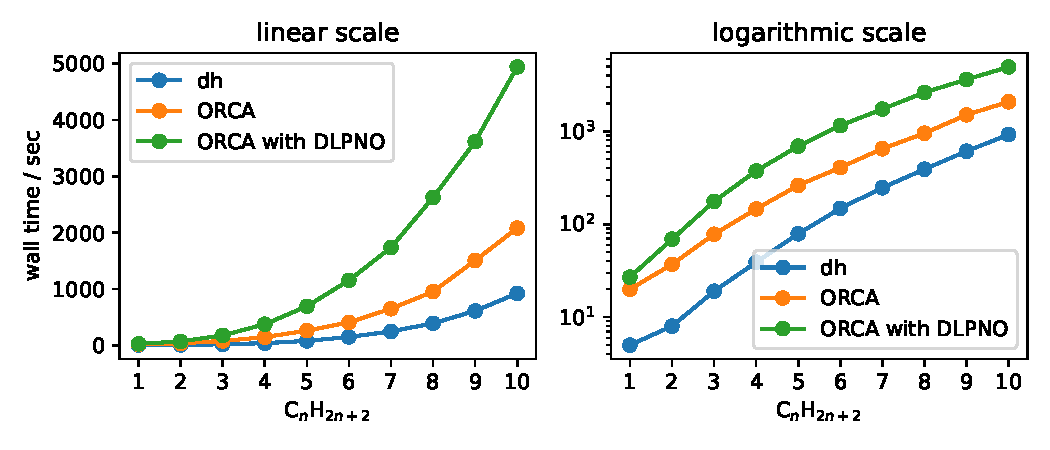
\includegraphics[width=0.8\textwidth]{assets/timing-polar-chain.pdf}
    \caption[\textsc{dh} 与 \textsc{ORCA} 程序计算 RI-MP2 静态极化率的效率测评]{\textsc{dh} 与 \textsc{ORCA} 程序计算 RI-MP2 静态极化率的效率测评。}
    \label{fig.3.timing-polar-chain}
\end{figure}

\textsc{dh} 程序的关键运行指令是\\
\verb|from pyscf import gto, dh|\\
\verb|from pyscf.dh.dipole.dh.rdh import RDHPolar|\\
\verb|mol = gto.Mole(..., basis="def2-QZVPPD", max_memory=320000)|\\
\verb|RDHPolar(mol, xc="MP2",|\\
\verb|    auxbasis_jk="def2-universal-jkfit",|\\
\verb|    auxbasis_ri="def2-QZVPPD-ri").run()|

\textsc{ORCA} 软件输入卡的关键参数设置是\\
\verb|! RI-MP2 RI-JK def2-QZVPPD def2/JK|\\
\verb|! def2-QZVPPD/C NoFrozenCore RITrafo|\\
\verb|%maxcore 8000|

对于 ORCA 实现的 DLPNO 方法,我们使用默认的 PNO 阈值。

\section{附录:非正则 MP2 相关能及其梯度}
\label{sec.3.non-canonical-mp2-gradient}

这一节的目的是给出 MP2 相关能在电性质下的导数。Aikens 等基于正则 SCF 下对 MP2 相关能作梯度推导与实现\cite{Aikens-Gordon.TCA.2003};在本工作的早期进展中也以该方式进行推演,并且由于计算程序的结果总是给出正则 SCF 下的结果,从而容易通过数值梯度验证解析梯度的公式推导与程序是否正确。但基于非正则 MP2 的情形以推演导数,比较容易清楚地区分 skeleton 导数和对轨道系数导数,并且自然地利用弱的正则 SCF 条件 (\ref{eq.3.weak-canonical-SCF}),消除 U 矩阵数值误差 (为避免 U 矩阵严重的数值误差,一阶梯度不适合使用强的正则 SCF 条件;而 Aikens 的推演过程依赖于正则情形下的 $\partial_\mathbb{A} \varepsilon_p$,为此需要花费精力与技巧合并求和值为零的、涉及 $U_{ij}^\mathbb{A}$ 和 $U_{ab}^\mathbb{A}$ 的同类项)。因而,非正则 MP2 从公式推演的角度上,会更清晰明了。

仅考虑闭壳层情形。同时,不同于正文,在 \ref{sec.3.non-canonical}--\ref{sec.3.coefficient-deriv} 小节中,性质量 $\mathbb{A}$ 与轨道系数 $\mathbf{C}$ 是去耦的 (即并非耦合微扰的,或者说 $\mathbf{C}$ 在这里不看作 $\mathbb{A}$ 的函数)。在 \ref{sec.3.amplitude-deriv} 小节将讨论 MP2 激发张量的全导数问题,此时的 $\mathbf{C}$ 将看作 $\mathbb{A}$ 的函数。

尽管 MP2 的相关能可以通过轨道能与轨道系数,一次性地计算得到;但在梯度推导中,尽管 Fock 矩阵本身 $F_{pq}$ 不管是程序实现还是公式推导中都将是对角的;但由于我们不要求 Fock 矩阵的导数 $\frac{\mathrm{d}}{\mathrm{d} \mathbb{A}} F_{pq}$ 也是对角矩阵,因此仍然需要关注非正则 SCF 情形下的 MP2 计算方式。

\subsection{非正则 MP2 相关能}
\label{sec.3.non-canonical}

对于闭壳层 MP2,非正则情形的能量与正则情形相同,都可以用激发系数与电子积分的乘积得到:
\begin{align}
    E_\textmt{c}^\textmt{(2)} &= T_{ij}^{ab} (ia|jb) \\
    T_{ij}^{ab} &= 2 t_{ij}^{ab} - t_{ij}^{ba}
\end{align}
但激发系数并非是正则情形下的 $t_{ij}^{ab} = (ia|jb) / D_{ij}^{ab}$,而是需要通过类似于 CISD 的迭代过程求解\cite{Pulay-Saeboe.TCA.1986}:
\begin{equation}
    \label{eq.3.non-canonical-mp2-working}
    (ia|jb) = F_{ki} t_{kj}^{ab} + F_{kj} t_{ik}^{ab} - F_{ca} t_{ij}^{cb} - F_{cb} t_{ij}^{ac} \quad \text{(non-canonical MP2)}
\end{equation}
为后续讨论的方便,定义辅助函数 $\symbfscr{H} (\mathbb{A}, \mathbf{C}, \mathbf{t})$;参数 $\mathbf{C}$ 是指自洽场系数 $C_{\mu p}$、$\mathbf{t}$ 是指 MP2 激发系数 $t_{ij}^{ab}$;辅助函数 $\symbfscr{H}$ 是四脚标张量 $\symscr{H}_{ij}^{ab}$:
\begin{empheq}[box=\fbox]{equation}
    \symscr{H}_{ij}^{ab} = F_{ki} t_{kj}^{ab} + F_{kj} t_{ik}^{ab} - F_{ca} t_{ij}^{cb} - F_{cb} t_{ij}^{ac} - (ia|jb) = 0 \quad \text{(non-canonical MP2)}
\end{empheq}
上述辅助函数的目的是为了求取激发张量 $\mathbf{t} (\mathbb{A}, \mathbf{C})$ 作为隐函数对轨道系数 $\mathbf{C}$ 或对性质量 $\mathbb{A}$ 的导数。对辅助函数 $\symbfscr{H} (\mathbb{A}, \mathbf{C}, \mathbf{t})$ 求偏导时,我们认为分子轨道基的 Fock 矩阵 $\mathbf{F}$ 依赖于性质量 $\mathbb{A}$ 与轨道系数 $\mathbf{C}$。

为后续讨论方便,仿照激发张量 $t_{ij}^{ab}$ 与闭壳层下的对偶正交激发张量 $T_{ij}^{ab}$,我们也定义分子轨道下 ERI 的张量与对偶正交 ERI 张量为
\begin{align}
    \label{eq.3.redef.g-ijab}
    g_{ij}^{ab} &= (ia|jb) \\
    G_{ij}^{ab} &= 2 g_{ij}^{ab} - g_{ij}^{ba}
\end{align}
在指标 $a, b$ 求和的前提下,容易证明对偶正交可以从激发张量迁移到 ERI 张量:
\begin{equation}
    E_\textmt{c}^\textmt{(2)} = T_{ij}^{ab} g_{ij}^{ab} = t_{ij}^{ab} G_{ij}^{ab}
\end{equation}
后续推导中经常使用类似的技巧。

\subsection{电性质一阶梯度:MP2 相关能对性质的 skeleton 导数}
\label{sec.3.skeleton}

本小节将给出 MP2 相关能的 skeleton 导数 $\partial_\mathbb{A}^\mathrm{S} E_\textmt{c}^\textmt{(2)}$。

对于电性质,skeleton 导数仅在涉及 Fock 矩阵或单电子积分矩阵、或者原子核互斥能时出现。对于分子轨道 ERI 积分 $g_{ij}^{ab}$,其 skeleton 导数为零。因此,MP2 相关能的 skeleton 导数为
\begin{equation}
    \label{eq.3.pdSA-Ec-MP2-0}
    \partial_\mathbb{A}^\mathrm{S} E_\textmt{c}^\textmt{(2)} = \frac{\partial E_\textmt{c}^\textmt{(2)} (\mathbb{A}, \mathbf{C})}{\partial \mathbb{A}} = \frac{\partial t_{ij}^{ab}}{\partial \mathbb{A}} G_{ij}^{ab}
\end{equation}
因此,对于 skeleton 导数,唯一需要关注的是激发张量 $t_{ij}^{ab}$ 在外场微扰 $\mathbb{A}$ 下的导数。

出于辅助函数 $\symbfscr{H} (\mathbb{A}, \mathbf{C}, \mathbf{t}) = \bm{0}$、以及轨道系数 $\mathbf{C}$ 在讨论 skeleton 导数时不发生变化,因此,
\begin{equation}
    \label{eq.3.auxfunc-pdA}
    \frac{\partial \symbfscr{H}}{\partial \mathbb{A}} + \frac{\partial \symbfscr{H}}{\partial \mathbf{t}} \frac{\partial \mathbf{t}}{\partial \mathbb{A}} = \bm{0}
\end{equation}
由于 Fock 矩阵不是 MP2 激发张量 $\mathbf{t}$ 的函数,因此讨论 $\partial_\mathbf{t} \symbfscr{H}$ 时,可以安全地引入正则 SCF 条件 $F_{pq} = \varepsilon_p \delta_{pq}$;在该情形下,
\begin{equation*}
    \symscr{H}_{ij}^{ab} = D_{ij}^{ab} t_{ij}^{ab} - (ia|jb) \quad \text{(when derivative not related to Fock matrix)}
\end{equation*}
$D_{ij}^{ab}$ 定义见式 (\ref{eq.3.def.d-ijab})。从而,对 $F_{ij}^{ab}$ 产生贡献的项一定是 $t_{ij}^{ab}$、而不会是激发张量 $\mathbf{t}$ 中其它元素。因此,
\begin{align}
    \label{eq.3.auxfunc-pdt}
    \frac{\partial \symscr{H}_{ij}^{ab}}{\partial t_{ij}^{ab}} &= D_{ij}^{ab} \\
    \frac{\partial \symscr{H}_{ij}^{ab}}{\partial t_{kl}^{cd}} &= 0 \quad (i,j,a,b \neq k,l,c,d)
\end{align}

对辅助函数 $\partial_\mathbb{A} \symbfscr{H}$ 产生贡献的仅有 Fock 矩阵的 skeleton 导数,因此
\begin{equation}
    \frac{\partial \symscr{H}_{ij}^{ab}}{\partial \mathbb{A}} = F_{ki}^\mathbb{A} t_{kj}^{ab} + F_{kj}^\mathbb{A} t_{ik}^{ab} - F_{ca}^\mathbb{A} t_{ij}^{cb} - F_{cb}^\mathbb{A} t_{ij}^{ac}
\end{equation}
联系式 (\ref{eq.3.auxfunc-pdA}),可以得到
\begin{equation}
    \frac{\partial t_{ij}^{ab}}{\partial \mathbb{A}} = - \frac{\displaystyle \frac{\partial \symscr{H}_{ij}^{ab}}{\partial \mathbb{A}}}{\displaystyle \frac{\partial \symscr{H}_{ij}^{ab}}{\partial t_{ij}^{ab}}} = \frac{- F_{ki}^\mathbb{A} t_{kj}^{ab} - F_{kj}^\mathbb{A} t_{ik}^{ab} + F_{ca}^\mathbb{A} t_{ij}^{cb} + F_{cb}^\mathbb{A} t_{ij}^{ac}}{D_{ij}^{ab}}
\end{equation}
代入式 (\ref{eq.3.pdSA-Ec-MP2-0}),并作指标对换与应用张量对称性,可以得到
\begin{empheq}[box=\fbox]{align}
    \partial_\mathbb{A}^\mathrm{S} E_\textmt{c}^\textmt{(2)} &= \left( - F_{ki}^\mathbb{A} t_{kj}^{ab} - F_{kj}^\mathbb{A} t_{ik}^{ab} + F_{ca}^\mathbb{A} t_{ij}^{cb} + F_{cb}^\mathbb{A} t_{ij}^{ac} \right) T_{ij}^{ab} \notag\\
    &= - 2 F_{ij}^\mathbb{A} T_{ik}^{ab} t_{jk}^{ab} + 2 F_{ab}^\mathbb{A} T_{ij}^{ac} t_{ij}^{bc}
\end{empheq}

通过上式,结合 (\ref{eq.3.collary.rdm-definition}) 附近的讨论,并且注意到对于电性质而言 $F_{pq}^\mathbb{A} = h_{pq}^\mathbb{A}$,那么可以通过 skeleton 导数给出 MP2 相关效应对约化密度矩阵的贡献:
\begin{subequations}
\begin{align}
    \label{eq.3.rdm-mp2-ij}
    D_{ij}^{\textmt{(2)}, \textmt{RDM}} &= - 2 T_{ik}^{ab} t_{jk}^{ab} \\
    \label{eq.3.rdm-mp2-ab}
    D_{ab}^{\textmt{(2)}, \textmt{RDM}} &= 2 T_{ij}^{ac} t_{ij}^{bc}
\end{align}
\end{subequations}
此情形下的约化密度是对称的。需要补充的是,一般来说约化密度矩阵的非占-占据和占据-非占不一定是零值;但由于 MP2 方法的一阶微扰波函数 $| \Psi^\textmt{(1)} \rangle$ 只含有二次激发波函数,使得对于 MP2 相关效应而言,$D_{ai}^{\textmt{(2)}, \textmt{RDM}} = D_{ia}^{\textmt{(2)}, \textmt{RDM}} = 0$。

\subsection{电性质一阶梯度:MP2 相关能对轨道系数的导数}
\label{sec.3.coefficient-deriv}

本小节将给出 MP2 相关效应对广义 Fock 矩阵 $\symscr{F}_{pq}^\textmt{(2)}$ 的贡献,以及对应的 Lagrangian $L_{ai}^\textmt{(2)}$。

MP2 相关能对轨道系数的梯度相关量写为 (乘以 $C_{\mu p}$ 是因为方便在分子轨道基下进行讨论)
\begin{equation}
    \label{eq.3.def-fock-cmp2}
    F_{mp}^\textmt{(2)} \coloneq C_{\mu m} \frac{\mathrm{d} E_\textmt{c}^\textmt{(2)}}{\mathrm{d} C_{\mu p}} = T_{ij}^{ab} C_{\mu m} \frac{\mathrm{d} g_{ij}^{ab}}{\mathrm{d} C_{\mu p}} + C_{\mu m} \frac{\mathrm{d} t_{ij}^{ab}}{\mathrm{d} C_{\mu p}} G_{ij}^{ab}
\end{equation}
上式定义了 $F_{mp}^\textmt{(2)}$ 即 MP2 相关能对广义 Fock 矩阵的贡献。

其中,ERI $g_{ij}^{ab}$ 的导数比较容易求得:
\begin{equation}
    C_{\mu m} \frac{\mathrm{d} g_{ij}^{ab}}{\mathrm{d} C_{\mu p}} = g_{mj}^{ab} \delta_{pi} + g_{im}^{ab} \delta_{pj} + g_{ij}^{mb} \delta_{pa} + g_{ij}^{am} \delta_{pb}
\end{equation}
从而,ERI 导数总相关能导数的贡献是
\begin{align}
    F_{mp}^\textmt{(2)} \leftarrow T_{ij}^{ab} C_{\mu m} \frac{\mathrm{d} g_{ij}^{ab}}{\mathrm{d} C_{\mu p}} &= T_{ij}^{ab} \big( g_{mj}^{ab} \delta_{pi} + g_{im}^{ab} \delta_{pj} + g_{ij}^{mb} \delta_{pa} + g_{ij}^{am} \delta_{pb} \big) \notag\\
    &= 2 T_{ij}^{ab} g_{mj}^{ab} \delta_{pi} + 2 T_{ij}^{ab} g_{ij}^{mb} \delta_{pa}
\end{align}
上式含 $\delta_{pj}$、$\delta_{pb}$ 的项在指标求和的前提下,可以分别归并到 $\delta_{pi}$、$\delta_{pa}$ 的项;以 $\delta_{pj}$ 为例,
\begin{align*}
    F_{mp}^\textmt{(2)} \leftarrow T_{ij}^{ab} g_{im}^{ab} \delta_{pj} = T_{ji}^{ba} g_{jm}^{ba} \delta_{pi} = T_{ij}^{ab} g_{mj}^{ab} \delta_{pi}
\end{align*}
上式推导的第一个等号利用 $i, j$ 与 $a, b$ 指标求和时交换、第二个等号利用张量对称性。由于使用 Kronecker delta 记号比较臃肿,我们也可以对 $p$ 是否为占据轨道或非占轨道进行分类讨论:
\begin{align}
    \label{eq.3.fock-cmp2-part1-mi}
    F_{mi}^\textmt{(2)} &\leftarrow 2 T_{ij}^{ab} g_{mj}^{ab} \\
    \label{eq.3.fock-cmp2-part1-ma}
    F_{ma}^\textmt{(2)} &\leftarrow 2 T_{ij}^{ab} g_{ij}^{mb}
\end{align}

激发张量对轨道系数 $\partial_\mathbf{C} \mathbf{t}$ 的求取稍复杂。出于辅助函数 $\symbfscr{H} (\mathbb{A}, \mathbf{C}, \mathbf{t}) = \bm{0}$、以及外加微扰 $\mathbb{A}$ 在讨论轨道系数导数时不发生变化,因此,
\begin{equation}
    \label{eq.3.auxfunc-pdC}
    \frac{\partial \symbfscr{H}}{\partial \mathbf{C}} + \frac{\partial \symbfscr{H}}{\partial \mathbf{t}} \frac{\partial \mathbf{t}}{\partial \mathbf{C}} = \bm{0}
\end{equation}
回顾式 (\ref{eq.3.auxfunc-pdC}, \ref{eq.3.auxfunc-pdt}),通过隐函数求导规则,可以推知 MP2 激发张量 $t_{ij}^{ab}$ 对轨道系数的导数是
\begin{align}
    \label{eq.3.relation-tpdc-fpdc}
    C_{\mu m} \frac{\partial t_{ij}^{ab}}{\partial C_{\mu r}}
    = - C_{\mu m} \frac{\partial \symscr{H}_{ij}^{ab}}{\partial C_{\mu r}} \left( \frac{\partial \symscr{H}_{ij}^{ab}}{\partial t_{ij}^{ab}} \right)^{-1}
    = - C_{\mu m} \frac{\partial \symscr{H}_{ij}^{ab}}{\partial C_{\mu r}} \frac{1}{D_{ij}^{ab}}
\end{align}
从而将 MP2 激发系数对轨道系数的导数 $\partial_\mathbf{C} \mathbf{t}$ 的求取问题,转化为辅助函数对轨道系数的导数 $\partial_\mathbf{C} \symbfscr{H}$ 的求取问题。

在进一步讨论前,先对 Fock 矩阵的导数作补充。回顾式 (\ref{eq.3.def.Auvkl}) 所给出的 Fock 矩阵对自洽场密度矩阵的导数,可以知道
\begin{align}
    C_{\mu m} \frac{\partial F_{pq}}{\partial C_{\mu r}} &= \delta_{pr} F_{mq} + \delta_{qr} F_{pm} + C_{\mu m} C_{\eta p} C_{\theta q} \frac{\partial F_{\eta \theta}}{\partial D_{\kappa \lambda}} \frac{\partial D_{\kappa \lambda}}{\partial C_{\mu r}} \notag\\
    &= \delta_{pr} F_{mq} + \delta_{qr} F_{pm} + \frac{1}{4} A_{pq, \kappa \lambda} C_{\mu m} \frac{\partial D_{\kappa \lambda}}{\partial C_{\mu r}}
\end{align}
上式临时使用了 $\eta, \theta$ 作为原子轨道指标。涉及自洽场密度矩阵 $D_{\kappa \lambda}$ 对轨道系数 $C_{\mu r}$ 导数的部分,注意到密度矩阵仅由占据轨道所决定 (同时注意到闭壳层是电子双占据的):
\begin{equation}
    \frac{\partial D_{\kappa \lambda}}{\partial C_{\mu r}} = \big( 2 \delta_{\kappa \mu} C_{\lambda r} + 2 \delta_{\lambda \mu} C_{\kappa r} \big) \delta_{r \in \mathrm{occ}}
\end{equation}
因此分类讨论比较方便。当指标 $r$ 指代非占轨道 $c$ 时,
\begin{equation}
    C_{\mu m} \frac{\partial F_{pq}}{\partial C_{\mu c}} = \delta_{pc} F_{mq} + \delta_{qc} F_{pm}
\end{equation}
当指标 $r$ 指代占据轨道 $k$ 时,注意到 A 张量的对称性,
\begin{equation}
    C_{\mu m} \frac{\partial F_{pq}}{\partial C_{\mu k}} = \delta_{pk} F_{mq} + \delta_{qk} F_{pm} + A_{pq, mk}
\end{equation}

随后可以考虑辅助函数对轨道系数的偏导数 $\partial_\mathbf{C} \symbfscr{H}$。经过一些简化,
\begin{subequations}
\begin{align}
    C_{\mu m} \frac{\partial \symscr{H}_{ij}^{ab}}{\partial C_{\mu k}} &= (\delta_{ki} F_{ml} + \delta_{kl} F_{mi} + A_{li, mk}) t_{lj}^{ab} + (\delta_{kj} F_{ml} + \delta_{kl} F_{mj} + A_{lj, mk}) t_{il}^{ab} \notag\\
    &\quad - A_{ca, mk} t_{ij}^{cb} - A_{cb, mk} t_{ij}^{ac} - \delta_{ki} g_{mj}^{ab} - \delta_{kj} g_{im}^{ab} \\
    C_{\mu m} \frac{\partial \symscr{H}_{ij}^{ab}}{\partial C_{\mu c}} &= - (\delta_{ca} F_{md} + \delta_{cd} F_{ma}) t_{ij}^{db} \notag\\
    &\quad - (\delta_{cb} F_{md} + \delta_{cd} F_{mb}) t_{ij}^{ad} - \delta_{ca} g_{ij}^{mb} - \delta_{cb} g_{ij}^{am}
\end{align}
\end{subequations}
依据式 (\ref{eq.3.relation-tpdc-fpdc}) 所给出的关系、张量对称性、求和时指标对换、引入正则 SCF 条件 $F_{pq} = \varepsilon_p \delta_{pq}$,将 $\partial_\mathbf{C} \mathbf{t}$ 并入式 (\ref{eq.3.def-fock-cmp2}) 第二项的计算将化简得到:
\begin{subequations}
\begin{align}
    \label{eq.3.fock-cmp2-part2-mk}
    F_{mk}^\textmt{(2)} &\leftarrow C_{\mu m} \frac{\mathrm{d} t_{ij}^{ab}}{\mathrm{d} C_{\mu k}} G_{ij}^{ab} = - C_{\mu m} \frac{\partial \symscr{H}_{ij}^{ab}}{\partial C_{\mu k}} T_{ij}^{ab} \notag\\
    &= - 4 \delta_{mi} \varepsilon_i T_{kj}^{ab} t_{ij}^{ab} + 2 T_{kj}^{ab} g_{mj}^{ab} - 2 A_{mk, il} T_{ij}^{ab} t_{lj}^{ab} + 2 A_{mk, ac} T_{ij}^{ab} t_{ij}^{cb} \\
    \label{eq.3.fock-cmp2-part2-mc}
    F_{mc}^\textmt{(2)} &\leftarrow C_{\mu m} \frac{\mathrm{d} t_{ij}^{ab}}{\mathrm{d} C_{\mu c}} G_{ij}^{ab} = - C_{\mu m} \frac{\partial \symscr{H}_{ij}^{ab}}{\partial C_{\mu c}} T_{ij}^{ab} \notag\\
    &= 4 \delta_{ma} \varepsilon_a T_{ij}^{cb} t_{ij}^{ab} + 2 T_{ij}^{ca} g_{ij}^{mb}
\end{align}
\end{subequations}
式 (\ref{eq.3.fock-cmp2-part2-mk}) 中,涉及到 A 张量的部分,可以用 MP2 相关约化密度 $D_{pq}^{(2),\textmt{RDM}}$ 简化。式 (\ref{eq.3.fock-cmp2-part2-mk}, \ref{eq.3.fock-cmp2-part2-mc}) 分别与式 (\ref{eq.3.fock-cmp2-part1-mi}, \ref{eq.3.fock-cmp2-part1-ma}) 结合,并经过一些指标置换,得到总的 MP2 相关效应对广义 Fock 矩阵的贡献:
\begin{subequations}
\begin{empheq}[box=\fbox]{align}
    \symscr{F}_{ij}^\textmt{(2)} &= 4 T_{ik}^{ab} g_{jk}^{ab} - 4 \varepsilon_j T_{ik}^{ab} t_{jk}^{ab} + A_{ij, pq} D_{pq}^{\textmt{(2)},\textmt{RDM}} \\
    \symscr{F}_{ai}^\textmt{(2)} &= 4 T_{ij}^{bc} g_{aj}^{bc} + A_{ai, pq} D_{pq}^{\textmt{(2)},\textmt{RDM}} \\
    \symscr{F}_{ia}^\textmt{(2)} &= 4 T_{jk}^{ab} g_{jk}^{ib} \\
    \symscr{F}_{ab}^\textmt{(2)} &= 4 T_{ij}^{ac} g_{ij}^{bc} + 4 \varepsilon_b T_{ij}^{ac} t_{ij}^{bc}
\end{empheq}
\end{subequations}
依式 (\ref{eq.3.def.lagrangian}),我们可以得到 MP2 相关效应对 Lagrangian 的贡献:
\begin{empheq}[box=\fbox]{equation}
    \label{eq.3.mp2-lagrangian}
    L_{ai}^\textmt{(2)} = \symscr{F}_{ai}^\textmt{(2)} - \symscr{F}_{ia}^\textmt{(2)} = 4 T_{ij}^{bc} g_{aj}^{bc} - 4 T_{jk}^{ab} g_{jk}^{ib} + A_{ai, pq} D_{pq}^{\textmt{(2)}, \textmt{RDM}}
\end{empheq}

如正文中式 (\ref{eq.3.derivation-contrib-Lai-to-engderiv}) 附近所讨论的,由于电性质梯度的 $U_{ij}^\mathbb{A}$ 与 $U_{ab}^\mathbb{A}$ 可以取零值;因此,广义 Fock 矩阵中,仅有占据-非占 $\symscr{F}_{ai}^\textmt{(2)}$ 和非占-占据 $\symscr{F}_{ai}^\textmt{(2)}$ 部分,对能量梯度有所贡献。但对于更一般的梯度问题,例如原子核坐标梯度,广义 Fock 矩阵的占据-占据 $\symscr{F}_{ij}^\textmt{(2)}$ 和非占-非占 $\symscr{F}_{ab}^\textmt{(2)}$ 部分将对能量加权密度矩阵 $W_{pq}$ 产生贡献 (见 Aikens 等式 (77--83)\cite{Aikens-Gordon.TCA.2003});进而该矩阵与重叠矩阵的 skeleton 导数 $S_{pq}^\mathbb{A}$ 作乘积对能量梯度产生贡献。

\subsection{电性质一阶梯度:MP2 激发张量全导数}
\label{sec.3.amplitude-deriv}

本小节将给出 MP2 激发张量的全导数 $\frac{\mathrm{d} \mathbf{t}}{\mathrm{d} \mathbb{A}}$;该量将用于 MP2 的二阶梯度计算中。

事实上,上两小节分别可以给出激发张量对性质的偏导数 (skeleton 导数) $\frac{\partial \mathbf{t}}{\partial \mathbb{A}}$ 与对轨道系数的偏导数 $\frac{\partial \mathbf{t}}{\partial \mathbf{C}}$;两者的加和就可以导出 $\frac{\mathrm{d} \mathbf{t}}{\mathrm{d} \mathbb{A}}$ (下式将激发系数 $\mathbf{t}$ 看作轨道系数 $\mathbf{C}$ 与性质 $\mathbb{A}$ 的函数):
\begin{equation*}
    \frac{\mathrm{d} t_{ij}^{ab}}{\mathrm{d} \mathbb{A}} = \frac{\partial t_{ij}^{ab}}{\partial \mathbb{A}} + \frac{\partial t_{ij}^{ab}}{\partial C_{\mu p}} \frac{\mathrm{d} C_{\mu p}}{\mathrm{d} \mathbb{A}}
\end{equation*}
但该表达式会比较复杂;在程序实现中,将使用下述方式给出激发张量全导数。

现在将轨道系数 $\mathbf{C}$ 与性质量 $\mathbb{A}$ 耦合;那么辅助函数将写为 $\symbfscr{H} (\mathbb{A}, \mathbf{t}) = 0$。仿照式 (\ref{eq.3.auxfunc-pdA}) 附近的推导;但同时注意到不同于 skeleton 导数的情形,$\frac{\mathrm{d}}{\mathrm{d} \mathbb{A}} (ia|jb)$ 作为全导数是非零的;那么容易得到
\begin{equation}
    \label{eq.3.pdA-tijab}
    \frac{\mathrm{d} t_{ij}^{ab}}{\mathrm{d} \mathbb{A}} = \frac{1}{D_{ij}^{ab}} \left(
    - \frac{\mathrm{d} F_{ki}}{\mathrm{d} \mathbb{A}} t_{kj}^{ab}
    - \frac{\mathrm{d} F_{kj}}{\mathrm{d} \mathbb{A}} t_{ik}^{ab}
    + \frac{\mathrm{d} F_{ca}}{\mathrm{d} \mathbb{A}} t_{ij}^{cb}
    + \frac{\mathrm{d} F_{cb}}{\mathrm{d} \mathbb{A}} t_{ij}^{ac}
    - \frac{\mathrm{d}}{\mathrm{d} \mathbb{A}} (ia|jb)
    \right)
\end{equation}

% 后文中,用于实现双杂化电性质梯度的程序是 dh (ver 80ca9e)。该程序仅在计算复杂度上有合理的表现;但出于实现便利与快速开发的目的,该程序并没有通过张量对称性、JIT 等策略加速程序。从图 \ref{fig.3.timing-rimp2-implemented} 中的表现来看,对于 RI-MP2 能量计算,dh 程序并未能发挥最高的效能。因% 此,我们预期未来
% 
% \subsection{重要的解析梯度先驱性工作}
% 
% 本工作的目标之一是高效率实现 RI 近似下 MP2 型 xDH 双杂化泛函的电性质二阶梯度;其理论推导与实现基于大量先驱性工作。其中,不完全的、具有代表性的或对本工作有一定影响的文献列举如下:
% \begin{itemize}[nosep]
%   \item Gerratt 与 Mills 在 1968 年发展了 Hartree-Fock 方法二阶梯度理论,并提出耦合微扰方程 (CPHF, \underline{C}oupled \underline{P}erturbed \underline{H}artree-\underline{F}ock)\cite{Gerratt-Mills.JCP.1968, Gerratt-Mills.JCP.1968a};
%   \item Pople 等在 1979 年发展了 MP2 方法的一阶梯度理论\cite{Pople-Binkley.IJQC.1979};
%   \item Dykstra 与 Jasien 在 1984 年发展了 Hartree-Fock 方法任意阶梯度理论,并提出了高阶轨道系数导数计算方法、与梯度理论的 $2n+1$ 规则\cite{Dykstra-Jasien.CPL.1984};
%   \item Handy 与 Schaefer III 在 1984 年发展了 CISD 方法四阶梯度理论,提出了 Z-Vector 方法,并指出 Z-Vector 方法在 MP2 等微扰方法下的应用前景\cite{Handy-Schaefer.JCP.1984};
%   \item Handy 在 1985 年针对轨道系数梯度矩阵中可能存在的奇点的问题,提出数值上更稳定的梯度计算方法\cite{Handy-Simandiras.CPL.1985};
%   \item Pulay 与 Saebø 在 1986 年提出 MP2 方法在非正则 Hartree-Fock 方法下的表达式,并指出该理论在二阶梯度下的应用前景\cite{Pulay-Saeboe.TCA.1986};
%   \item Frisch、Head-Gordon、Pople 在 1990 年基于 Gaussian 程序实现了 Hartree-Fock 方法的二阶梯度与 MP2 方法的一阶梯度\cite{Frisch-Pople.CP.1990, Frisch-Pople.CPL.1990, Frisch-Pople.CPL.1990a};
%   \item Bartlett、Gauss 与 Stanton 在 1992 年基于 ACES II 程序 (后期发展为 CFOUR) 实现了 MP2 方法的二阶梯度\cite{Gauss-Bartlett.JCP.1992, Stanton-Bartlett.CPL.1992};
%   \item Johnson 与 Frisch 在 1993 年基于 Gaussian 程序实现了 GGA 泛函的二阶梯度\cite{Johnson-Frisch.CPL.1993};
%   \item Head-Gordon 与 Head-Gordon 在 1994 年基于 Gaussian 程序实现了 MP2 方法的二阶梯度\cite{Head-Gordon-Head-Gordon.CPL.1994};
%   \item Yamaguchi、Goddard、Osamura 与 Schaefer III 在 1994 年对变分方法下的梯度理论作全面的总结\cite{Yamaguchi-Schaefer.Oxford.1994};
%   \item Weigend 与 H\"aser 在 1997 年发展并基于 TURBOMOLE 程序实现了 RI-MP2 方法的一阶梯度\cite{Weigend-Haeser.TCA.1997};
%   \item Gordon 课题组 Aikens 等在 2004 年发展并基于 GAMESS US 程序实现了冻结轨道的 MP2 方法一阶梯度\cite{Aikens-Gordon.TCA.2003};
%   \item Cammi 等在 2004 年发展并基于 Gaussian 程序实现了溶剂化 MP2 方法二阶梯度\cite{Cammi-Frisch.TCA.2004};
%   \item Head-Gordon 课题组 Distasio, Jr.\ 等在 2007 年基于 Q-Chem 程序实现了 RI-MP2 方法的一阶梯度\cite{Distasio-Head-Gordon.JCC.2007};
%   \item Neese、Schwabe 与 Grimme 在 2007 年发展并基于 ORCA 程序实现了 MP2 型 bDH 双杂化泛函的一阶梯度\cite{Neese-Grimme.JCP.2007};
%   \item Biczysko 等在 2010 年发展并基于 Gaussian 程序实现了 MP2 型 bDH 双杂化泛函二阶梯度\cite{Biczysko-Barone.JCTC.2010};
%   \item 苏乃强、张颖、徐昕在 2013 年发展并基于 NWChem 程序实现了 MP2 型 xDH 双杂化泛函一阶梯度\cite{Su-Xu.JCC.2013};
%   \item Jung 课题组 Ji 等在 2013 年发展并基于 Q-Chem 程序实现了 Laplace-Transform 近似 ($1/x$ 的指数函数展开近似) OS-MP2 型 xDH 双杂化泛函一阶梯度\cite{Ji-Jung.JCTC.2013};
%   \item Neese 课题组 Bykov 等与 Valeev 合作在 2015 年发展并基于 ORCA 程序实现了 RIJ-COSX 近似下的二阶梯度,并高效实现了 RI 近似下自洽场的二阶梯度\cite{Bykov-Neese.MP.2015};
%   \item Stoychev、Auer 与 Neese 在 2018 年发展并基于 ORCA 程序实现了 RI-MP2 以及 RI 近似下 MP2 型 bDH 双杂化泛函电性质和磁性质二阶梯度\cite{Stoychev-Neese.JCTC.2018};
%   \item 谷永浩、祝震予、徐昕在 2021 年发展并基于 Gaussian 程序实现了 MP2 型 xDH 双杂化泛函振动频率与极化率二阶梯度\cite{Gu-Xu.JCTC.2021}。
%   \item 颜文杰、徐昕在 2022 年发展并基于 Gaussian 程序实现了 MP2 型 xDH 双杂化泛函磁化率与核磁矩二阶梯度\cite{Yan-Xu.JCTC.2022}。
% \end{itemize}



